\documentclass[10pt,a4paper]{article}

\usepackage[margin=0.75cm]{geometry}
\usepackage[utf8]{inputenc}

\usepackage{amsmath}
\usepackage{amssymb}
\usepackage{biblatex}
\usepackage{textcomp}
\usepackage{gensymb}
\usepackage{paracol}
\usepackage{parskip}
\usepackage{tikz}
\usepackage{titlesec}
\usepackage{verbatim}
\usepackage{xcolor}

\titleformat{\section}[block]{\Large\bfseries\filcenter\color{red}}{\thesection}{1em}{}[\hrule]
\titleformat{\subsection}[block]{\bfseries\filcenter\color{red}}{\thesubsection}{1em}{}[\hrule]

\setlength{\columnsep}{25pt}

\tikzset{
    rounded-box/.style = {draw=red, fill=white, thin, rectangle, rounded corners, inner sep=5pt, inner ysep=10pt},
    rounded-box-title/.style = {fill=red, text=white, font=\bfseries},
}

\addbibresource{references.bib}

\begin{document}
\title{Linear Algebra}

\section{Vectors}

\begin{paracol}{2}

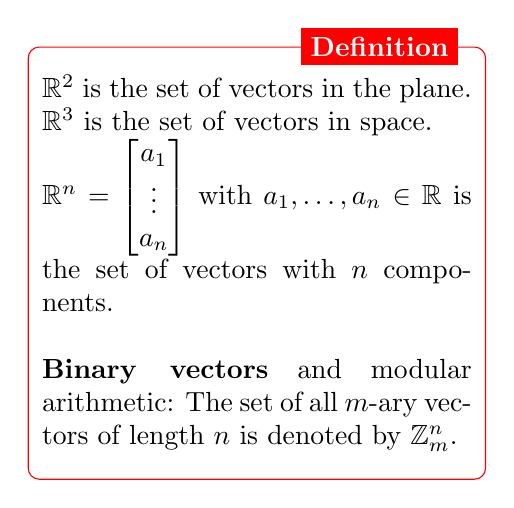
\begin{tikzpicture}
\node [rounded-box] (box){\begin{minipage}{0.45\textwidth}
    $\mathbb{R}^2$ is the set of vectors in the plane.

    $\mathbb{R}^3$ is the set of vectors in space.

    $\mathbb{R}^n = \begin{bmatrix} a_1 \\ \vdots \\ a_n \end{bmatrix}$ with $a_1, \dots, a_n \in \mathbb{R}$ is the set of vectors with $n$ components. \\

    \textbf{Binary vectors} and modular arithmetic: The set of all $m$-ary vectors of length $n$ is denoted by $\mathbb{Z}_m^n$.
\end{minipage}};
\node[rounded-box-title, left=10pt] at (box.north east) {Definition};
\end{tikzpicture}

\switchcolumn

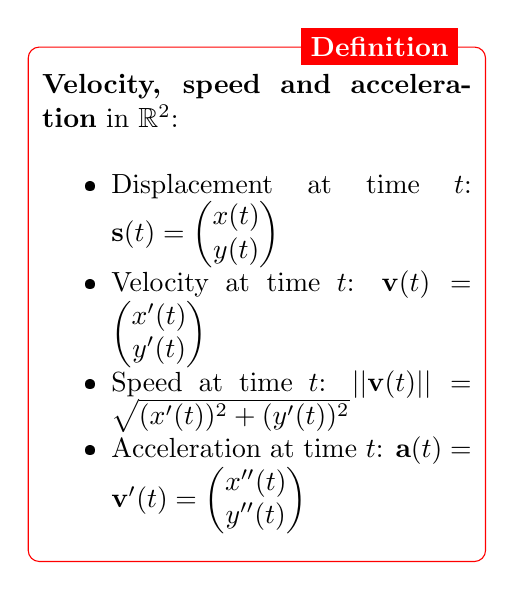
\begin{tikzpicture}
\node [rounded-box] (box){\begin{minipage}{0.45\textwidth}
    \textbf{Velocity, speed and acceleration} in $\mathbb{R}^2$: \\

    \begin{itemize}
        \item Displacement at time $t$: $\mathbf{s}(t) = \begin{pmatrix}
            x(t) \\ y(t)
        \end{pmatrix}$
        \item Velocity at time $t$: $\mathbf{v}(t) = \begin{pmatrix}
            x'(t) \\ y'(t)
        \end{pmatrix}$
        \item Speed at time $t$: $|| \mathbf{v}(t) || = \sqrt{(x'(t))^2 + (y'(t))^2}$
        \item Acceleration at time $t$: $\mathbf{a}(t) = \mathbf{v}'(t) = \begin{pmatrix}
            x''(t) \\ y''(t)
        \end{pmatrix}$
    \end{itemize}
\end{minipage}};
\node[rounded-box-title, left=10pt] at (box.north east) {Definition};
\end{tikzpicture}

\end{paracol}

\subsection{The Dot Product}

\begin{paracol}{2}

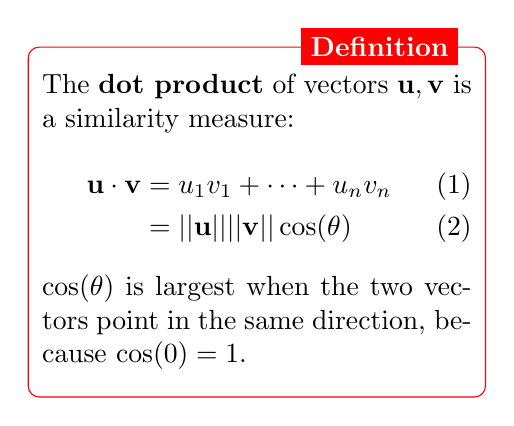
\begin{tikzpicture}
\node [rounded-box] (box){\begin{minipage}{0.45\textwidth}
    The \textbf{dot product} of vectors $\mathbf{u}, \mathbf{v}$ is a similarity measure:

    \vspace{-10pt}

    \begin{align}
        \mathbf{u} \cdot \mathbf{v} & = u_1 v_1 + \dots + u_n v_n \\
            & = || \mathbf{u} || || \mathbf{v} || \cos(\theta)
    \end{align}

    $\cos(\theta)$ is largest when the two vectors point in the same direction, because $\cos(0) = 1$.
\end{minipage}};
\node[rounded-box-title, left=10pt] at (box.north east) {Definition};
\end{tikzpicture}

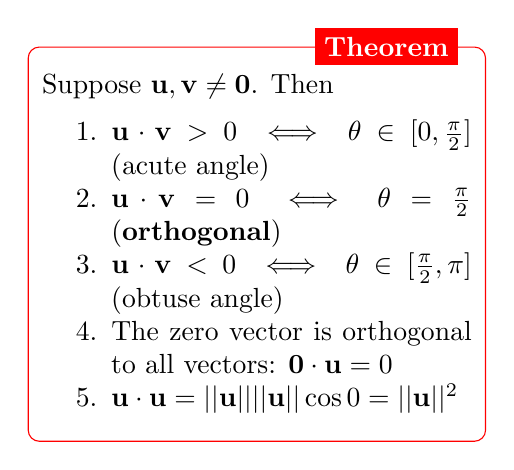
\begin{tikzpicture}
\node [rounded-box] (box){\begin{minipage}{0.45\textwidth}
    Suppose $\mathbf{u}, \mathbf{v} \neq \mathbf{0}$. Then

    \vspace{5pt}

    \begin{enumerate}
        \item $\mathbf{u} \cdot \mathbf{v} > 0 \iff \theta \in [0, \frac{\pi}{2}]$ \quad (acute angle)
        \item $\mathbf{u} \cdot \mathbf{v} = 0 \iff \theta = \frac{\pi}{2}$ \hspace{11pt} \quad (\textbf{orthogonal})
        \item $\mathbf{u} \cdot \mathbf{v} < 0 \iff \theta \in [\frac{\pi}{2}, \pi]$ \quad (obtuse angle)
        \item The zero vector is orthogonal to all vectors: $\mathbf{0} \cdot \mathbf{u} = 0$
        \item $\mathbf{u} \cdot \mathbf{u} = || \mathbf{u} || || \mathbf{u} || \cos{0} =  || \mathbf{u} ||^2$
    \end{enumerate}
\end{minipage}};
\node[rounded-box-title, left=10pt] at (box.north east) {Theorem};
\end{tikzpicture}

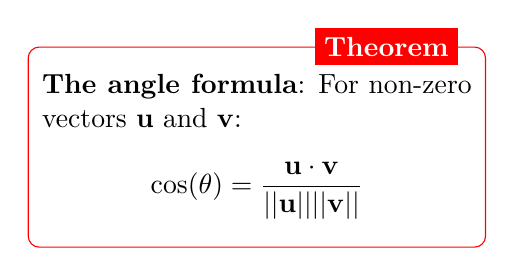
\begin{tikzpicture}
\node [rounded-box] (box){\begin{minipage}{0.45\textwidth}
    \textbf{The angle formula}: For non-zero vectors $\mathbf{u}$ and $\mathbf{v}$:

    $$\cos(\theta) = \frac{\mathbf{u} \cdot \mathbf{v}}{|| \mathbf{u} || || \mathbf{v} ||}$$
\end{minipage}};
\node[rounded-box-title, left=10pt] at (box.north east) {Theorem};
\end{tikzpicture}

\switchcolumn

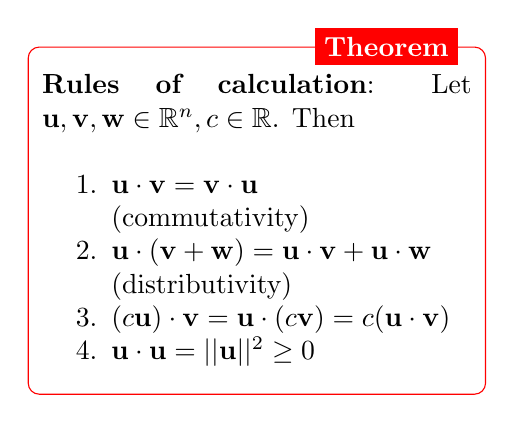
\begin{tikzpicture}
\node [rounded-box] (box){\begin{minipage}{0.45\textwidth}
    \textbf{Rules of calculation}: Let $\mathbf{u}, \mathbf{v}, \mathbf{w} \in \mathbb{R}^n, c \in \mathbb{R}$. Then \\

    \begin{enumerate}
        \item \makebox[4.5cm][l]{$\mathbf{u} \cdot \mathbf{v} = \mathbf{v} \cdot \mathbf{u}$} \quad (commutativity)
        \item \makebox[4.5cm][l]{$\mathbf{u} \cdot (\mathbf{v} + \mathbf{w}) = \mathbf{u} \cdot \mathbf{v} + \mathbf{u} \cdot \mathbf{w}$} \quad (distributivity)
        \item $(c \mathbf{u}) \cdot \mathbf{v} = \mathbf{u} \cdot (c \mathbf{v}) = c (\mathbf{u} \cdot \mathbf{v})$
        \item $\mathbf{u} \cdot \mathbf{u} = || \mathbf{u} ||^2 \geq 0$
    \end{enumerate}
\end{minipage}};
\node[rounded-box-title, left=10pt] at (box.north east) {Theorem};
\end{tikzpicture}

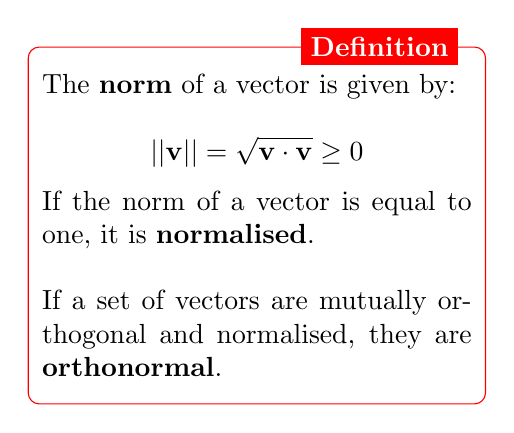
\begin{tikzpicture}
\node [rounded-box] (box){\begin{minipage}{0.45\textwidth}
    The \textbf{norm} of a vector is given by:

    $$|| \mathbf{v} || = \sqrt{\mathbf{v} \cdot \mathbf{v}} \geq 0$$

    If the norm of a vector is equal to one, it is \textbf{normalised}. \\

    If a set of vectors are mutually orthogonal and normalised, they are \textbf{orthonormal}.
\end{minipage}};
\node[rounded-box-title, left=10pt] at (box.north east) {Definition};
\end{tikzpicture}

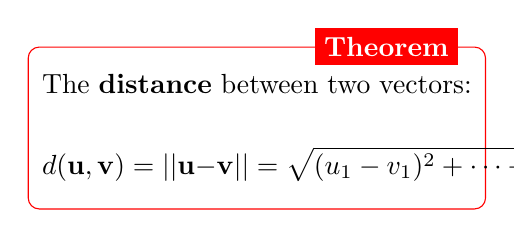
\begin{tikzpicture}
\node [rounded-box] (box){\begin{minipage}{0.45\textwidth}
    The \textbf{distance} between two vectors:

    \vspace{-5pt}

    $$d(\mathbf{u}, \mathbf{v}) = || \mathbf{u} - \mathbf{v} || = \sqrt{(u_1 - v_1)^2 + \dots + (u_n - v_n)^2}$$
\end{minipage}};
\node[rounded-box-title, left=10pt] at (box.north east) {Theorem};
\end{tikzpicture}

\end{paracol}

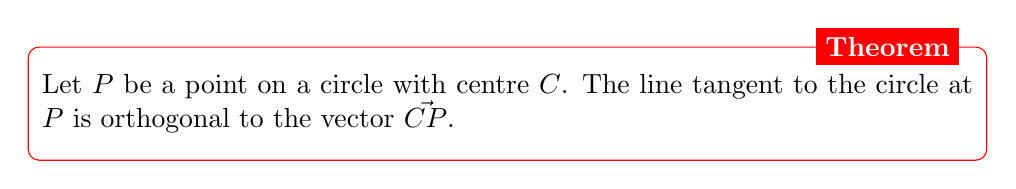
\begin{tikzpicture}
\node [rounded-box] (box){\begin{minipage}{0.975\textwidth}
    Let $P$ be a point on a circle with centre $C$. The line tangent to the circle at $P$ is orthogonal to the vector $\vec{CP}$.
\end{minipage}};
\node[rounded-box-title, left=10pt] at (box.north east) {Theorem};
\end{tikzpicture}

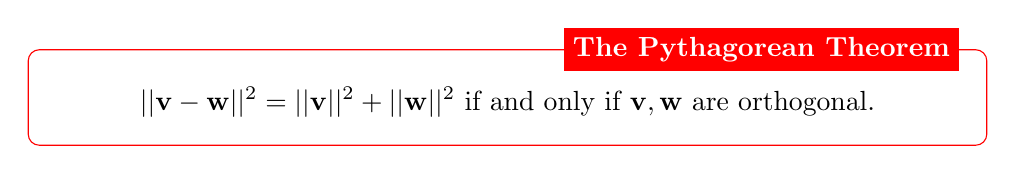
\begin{tikzpicture}
\node [rounded-box] (box){\begin{minipage}{0.975\textwidth}
    $$||\mathbf{v} - \mathbf{w}||^2 = ||\mathbf{v}||^2 + ||\mathbf{w}||^2 \text{ if and only if } \mathbf{v}, \mathbf{w} \text{ are orthogonal.}$$
\end{minipage}};
\node[rounded-box-title, left=10pt] at (box.north east) {The Pythagorean Theorem};
\end{tikzpicture}

\textbf{Proof}:

\vspace{-40pt}

\begin{align}
||\mathbf{v} - \mathbf{w}||^2 & = (\mathbf{v} - \mathbf{w}) \cdot (\mathbf{v} - \mathbf{w}) & \\
    & = \mathbf{v} \cdot \mathbf{v} + \mathbf{v} \cdot (- \mathbf{w}) + (- \mathbf{w}) \cdot \mathbf{v} + (- \mathbf{w}) \cdot (- \mathbf{w}) & \text{by rule 2} \\
    & = \mathbf{v} \cdot \mathbf{v} - 2 \mathbf{v} \cdot \mathbf{w} + \mathbf{w} \cdot \mathbf{w} & \text{by rules 1 and 2} \\
    & = ||\mathbf{v}||^2 - 2 \mathbf{v} \cdot \mathbf{w} + ||\mathbf{w}||^2 & \\
    & = ||\mathbf{v}||^2 + ||\mathbf{w}||^2 & \text{ if and only if }\mathbf{v} \cdot \mathbf{w} = 0
\end{align}

\begin{paracol}{2}


\begin{tikzpicture}
\node [rounded-box] (box){\begin{minipage}{0.45\textwidth}
    $$| \mathbf{u} \cdot \mathbf{v} | \leq || \mathbf{u} || || \mathbf{v} ||$$
\end{minipage}};
\node[rounded-box-title, left=10pt] at (box.north east) {Cauchy-Schwarz Inequality};
\end{tikzpicture}

\textbf{Proof}: TODO

\switchcolumn

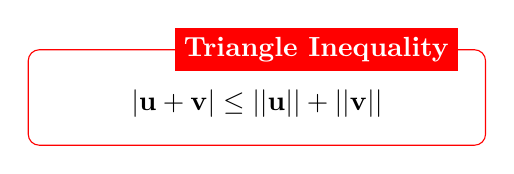
\begin{tikzpicture}
\node [rounded-box] (box){\begin{minipage}{0.45\textwidth}
    $$| \mathbf{u} + \mathbf{v} | \leq || \mathbf{u} || + || \mathbf{v} ||$$
\end{minipage}};
\node[rounded-box-title, left=10pt] at (box.north east) {Triangle Inequality};
\end{tikzpicture}

\textbf{Proof}: TODO

\end{paracol}

\newpage

\subsection{The Cross Product}

\begin{paracol}{2}

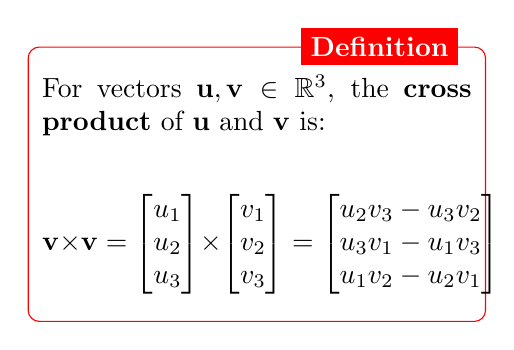
\begin{tikzpicture}
\node [rounded-box] (box){\begin{minipage}{0.45\textwidth}
    For vectors $\mathbf{u}, \mathbf{v} \in \mathbb{R}^3$, the \textbf{cross product} of $\mathbf{u}$ and $\mathbf{v}$ is:

    $$\mathbf{v} \times \mathbf{v} = \begin{bmatrix}
        u_1 \\ u_2 \\ u_3
    \end{bmatrix} \times \begin{bmatrix}
        v_1 \\ v_2 \\ v_3
    \end{bmatrix} = \begin{bmatrix}
        u_2 v_3 - u_3 v_2 \\
        u_3 v_1 - u_1 v_3 \\
        u_1 v_2 - u_2 v_1
    \end{bmatrix}$$
\end{minipage}};
\node[rounded-box-title, left=10pt] at (box.north east) {Definition};
\end{tikzpicture}

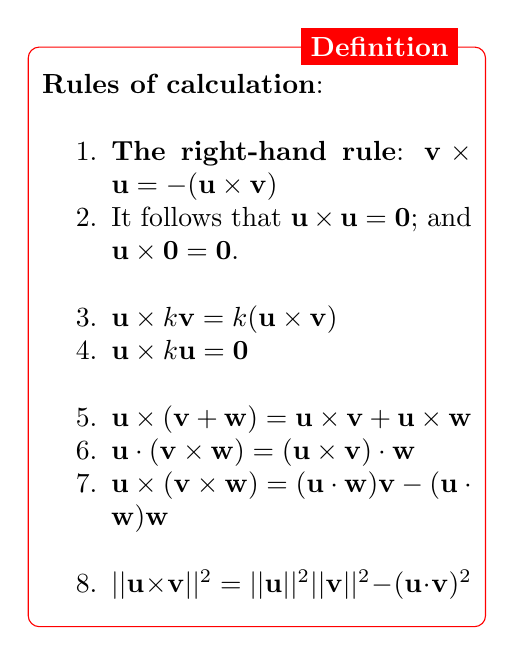
\begin{tikzpicture}
\node [rounded-box] (box){\begin{minipage}{0.45\textwidth}
    \textbf{Rules of calculation}: \\

    \begin{enumerate}
        \item \textbf{The right-hand rule}: $\mathbf{v} \times \mathbf{u} = - (\mathbf{u} \times \mathbf{v})$
        \item It follows that $\mathbf{u} \times \mathbf{u} = \mathbf{0}$; and $\mathbf{u} \times \mathbf{0} = \mathbf{0}$. \\

        \item $\mathbf{u} \times k \mathbf{v} = k (\mathbf{u} \times \mathbf{v})$
        \item $\mathbf{u} \times k \mathbf{u} = \mathbf{0}$ \\

        \item $\mathbf{u} \times (\mathbf{v} + \mathbf{w}) = \mathbf{u} \times \mathbf{v} + \mathbf{u} \times \mathbf{w}$
        \item $\mathbf{u} \cdot (\mathbf{v} \times \mathbf{w}) = (\mathbf{u} \times \mathbf{v}) \cdot \mathbf{w}$
        \item $\mathbf{u} \times (\mathbf{v} \times \mathbf{w}) = (\mathbf{u} \cdot \mathbf{w}) \mathbf{v} - (\mathbf{u} \cdot \mathbf{w}) \mathbf{w}$ \\

        \item $|| \mathbf{u} \times \mathbf{v} ||^2 = || \mathbf{u} ||^2 || \mathbf{v} ||^2 - (\mathbf{u} \cdot \mathbf{v})^2$
    \end{enumerate}
\end{minipage}};
\node[rounded-box-title, left=10pt] at (box.north east) {Definition};
\end{tikzpicture}

\switchcolumn

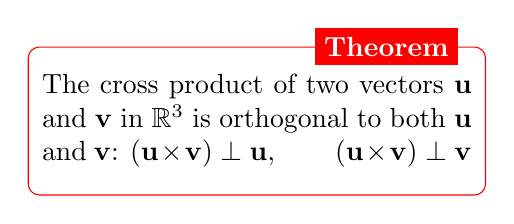
\begin{tikzpicture}
\node [rounded-box] (box){\begin{minipage}{0.45\textwidth}
    The cross product of two vectors $\mathbf{u}$ and $\mathbf{v}$ in $\mathbb{R}^3$ is orthogonal to both $\mathbf{u}$ and $\mathbf{v}$: $(\mathbf{u} \times \mathbf{v}) \perp \mathbf{u}, \qquad (\mathbf{u} \times \mathbf{v}) \perp \mathbf{v}$
\end{minipage}};
\node[rounded-box-title, left=10pt] at (box.north east) {Theorem};
\end{tikzpicture}

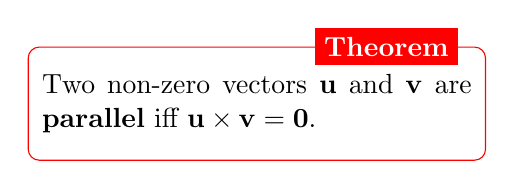
\begin{tikzpicture}
\node [rounded-box] (box){\begin{minipage}{0.45\textwidth}
    Two non-zero vectors $\mathbf{u}$ and $\mathbf{v}$ are \textbf{parallel} iff $\mathbf{u} \times \mathbf{v} = \mathbf{0}$.
\end{minipage}};
\node[rounded-box-title, left=10pt] at (box.north east) {Theorem};
\end{tikzpicture}

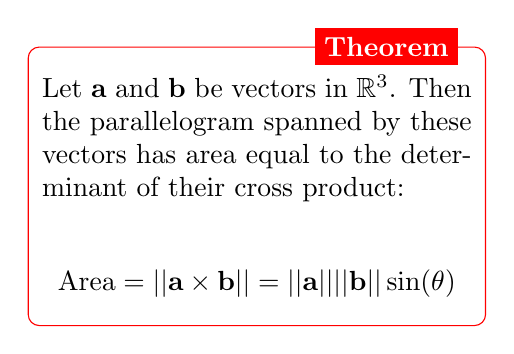
\begin{tikzpicture}
\node [rounded-box] (box){\begin{minipage}{0.45\textwidth}
    Let $\mathbf{a}$ and $\mathbf{b}$ be vectors in $\mathbb{R}^3$. Then the parallelogram spanned by these vectors has area equal to the determinant of their cross product:

    $$\text{Area} = || \mathbf{a} \times \mathbf{b} || = || \mathbf{a} || || \mathbf{b} || \sin(\theta)$$
\end{minipage}};
\node[rounded-box-title, left=10pt] at (box.north east) {Theorem};
\end{tikzpicture}

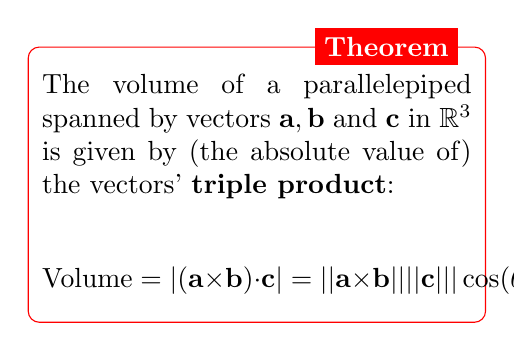
\begin{tikzpicture}
\node [rounded-box] (box){\begin{minipage}{0.45\textwidth}
    The volume of a parallelepiped spanned by vectors $\mathbf{a}, \mathbf{b}$ and $\mathbf{c}$ in $\mathbb{R}^3$ is given by (the absolute value of) the vectors' \textbf{triple product}:

    $$\text{Volume} = | (\mathbf{a} \times \mathbf{b}) \cdot \mathbf{c} | = || \mathbf{a} \times \mathbf{b} || || \mathbf{c} || | \cos(\theta) |$$
\end{minipage}};
\node[rounded-box-title, left=10pt] at (box.north east) {Theorem};
\end{tikzpicture}

\end{paracol}

\vspace{-10pt}

\subsection{Lines and Planes}

\begin{paracol}{2}

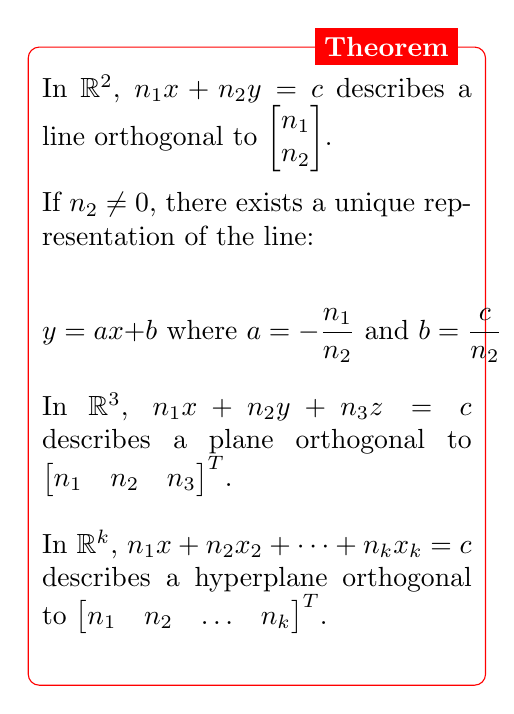
\begin{tikzpicture}
\node [rounded-box] (box){\begin{minipage}{0.45\textwidth}
    In $\mathbb{R}^2$, $n_1 x + n_2 y = c$ describes a line orthogonal to $\begin{bmatrix}
        n_1 \\ n_2
    \end{bmatrix}$. \\

    If $n_2 \neq 0$, there exists a unique representation of the line:

    $$y = a x + b \text{ where } a = - \frac{n_1}{n_2} \text{ and } b = \frac{c}{n_2}$$

    In $\mathbb{R}^3$, $n_1 x + n_2 y + n_3 z = c$ describes a plane orthogonal to $\begin{bmatrix}
        n_1 & n_2 & n_3
    \end{bmatrix}^T$. \\

    In $\mathbb{R}^k$, $n_1 x + n_2 x_2 + \dots + n_k x_k = c$ describes a hyperplane orthogonal to $\begin{bmatrix}
        n_1 & n_2 & \dots & n_k
    \end{bmatrix}^T$. \\
\end{minipage}};
\node[rounded-box-title, left=10pt] at (box.north east) {Theorem};
\end{tikzpicture}

\switchcolumn

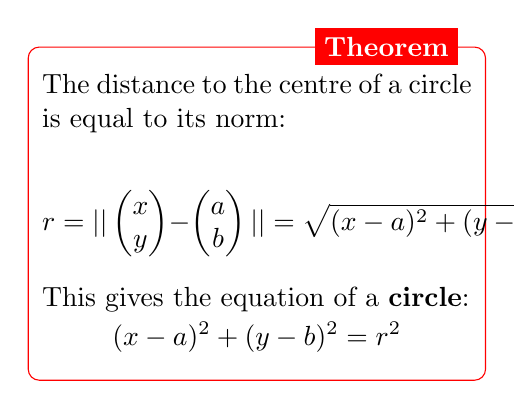
\begin{tikzpicture}
\node [rounded-box] (box){\begin{minipage}{0.45\textwidth}
    The distance to the centre of a circle is equal to its norm:

    $$
    r = || \begin{pmatrix}
        x \\ y
    \end{pmatrix} - \begin{pmatrix}
        a \\ b
    \end{pmatrix} || = \sqrt{(x-a)^2 + (y-b)^2}
    $$

    This gives the equation of a \textbf{circle}:

    \vspace{-10pt}

    $$(x-a)^2 + (y-b)^2 = r^2$$
\end{minipage}};
\node[rounded-box-title, left=10pt] at (box.north east) {Theorem};
\end{tikzpicture}

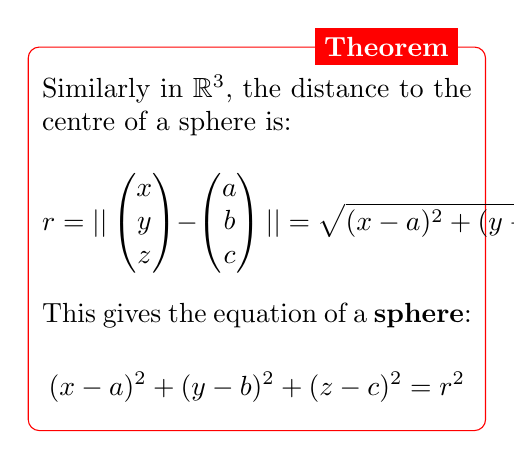
\begin{tikzpicture}
\node [rounded-box] (box){\begin{minipage}{0.45\textwidth}
    Similarly in $\mathbb{R}^3$, the distance to the centre of a sphere is:

    \vspace{-7.5pt}

    $$
    r = || \begin{pmatrix}
        x \\ y \\ z
    \end{pmatrix} - \begin{pmatrix}
        a \\ b \\ c
    \end{pmatrix} || = \sqrt{(x-a)^2 + (y-b)^2 + (z-c)^2}
    $$

    This gives the equation of a \textbf{sphere}:

    \vspace{-7.5pt}

    $$(x-a)^2 + (y-b)^2 + (z-c)^2 = r^2$$
\end{minipage}};
\node[rounded-box-title, left=10pt] at (box.north east) {Theorem};
\end{tikzpicture}

\switchcolumn

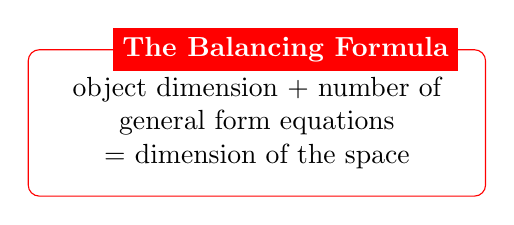
\begin{tikzpicture}
\node [rounded-box] (box){\begin{minipage}{0.45\textwidth}
    \begin{center}
        object dimension + number of general form equations
        
        = dimension of the space
    \end{center}
\end{minipage}};
\node[rounded-box-title, left=10pt] at (box.north east) {The Balancing Formula};
\end{tikzpicture}

\end{paracol}

\vspace{-10pt}

\begin{center}
\begin{tabular}{c|c|c|c|c}
    & Normal Form & General Form & Vector Form & Parametric Form \\
    \hline
    Lines in $\mathbb{R}^2$ & $\mathbf{n} \cdot ( \mathbf{x} - \mathbf{x} ) = \mathbf{0} \iff \mathbf{n} \cdot \mathbf{x} = \mathbf{n} \cdot \mathbf{p}$ & $n_1 x + n_2 y = c$  & $\mathbf{x} = \mathbf{p} + t \mathbf{v}$ & $\begin{cases}
        x = p_1 + t v1 \\
        y = p_2 + t v2
    \end{cases}$ \\
    \hline
    Lines in $\mathbb{R}^3$ & $\begin{cases}
        \mathbf{n}_1 \cdot \mathbf{x} = \mathbf{n}_1 \cdot \mathbf{p}_1 \\
        \mathbf{n}_2 \cdot \mathbf{x} = \mathbf{n}_2 \cdot \mathbf{p}_2
    \end{cases}$ & $\begin{cases}
        n_1{_1} x + n_1{_2} y + n_1{_3} z = c_1 \\
        n_2{_1} x + n_2{_2} y + n_2{_3} z = c_2
    \end{cases}$ & $\mathbf{x} = \mathbf{p} + t \mathbf{v}$ & $\begin{cases}
        x = p_1 + t v1 \\
        y = p_2 + t v2 \\
        z = p_3 + t v3
    \end{cases}$ \\
    \hline
    Planes in $\mathbb{R}^3$ & $\mathbf{n} \cdot ( \mathbf{x} - \mathbf{p} ) = \mathbf{0} \iff \mathbf{n} \cdot \mathbf{x} = \mathbf{n} \cdot \mathbf{p}$ & $n_1 x + n_2 y + n_3 z = c$  & $\mathbf{x} = \mathbf{p} + s \mathbf{u} + t \mathbf{v}$ & $\begin{cases}
        x = p_1 + s u_1 + t v_1 \\
        y = p_2 + s u_2 + t v_2 \\
        z = p_3 + s u_3 + t v_3
    \end{cases}$
\end{tabular}
\end{center}

$\mathbf{n} \neq \mathbf{0}$ is a normal vector. $\mathbf{p}$ is a given point on the line / in the plane. $\mathbf{u}, \mathbf{v} \neq \mathbf{0}$ are direction vectors of the line / plane.

\begin{paracol}{2}

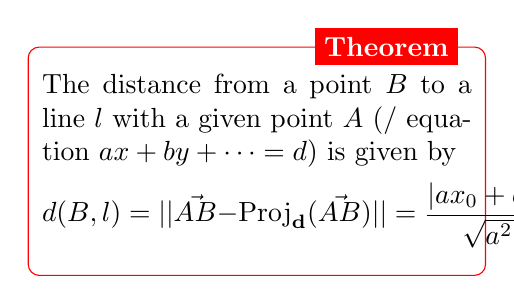
\begin{tikzpicture}
\node [rounded-box] (box){\begin{minipage}{0.45\textwidth}
    The distance from a point $B$ to a line $l$ with a given point $A$ (/ equation $ax + by + \dots = d$) is given by

    \vspace{-15pt}

    $$d(B, l) = || \vec{AB} - \text{Proj}_\mathbf{d}(\vec{AB}) || = \frac{| a x_0 + b y_0 + \dots - d |}{\sqrt{a^2 + b^2 + \dots}}$$
\end{minipage}};
\node[rounded-box-title, left=10pt] at (box.north east) {Theorem};
\end{tikzpicture}

\switchcolumn

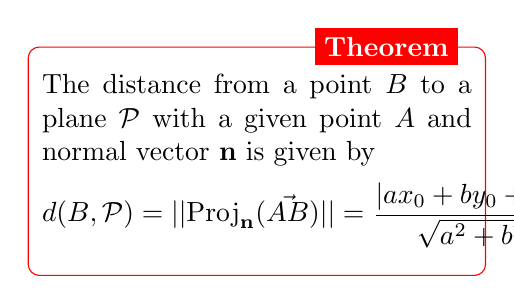
\begin{tikzpicture}
\node [rounded-box] (box){\begin{minipage}{0.45\textwidth}
    The distance from a point $B$ to a plane $\mathcal{P}$ with a given point $A$ and normal vector $\mathbf{n}$ is given by

    \vspace{-15pt}

    $$d(B, \mathcal{P}) = || \text{Proj}_\mathbf{n}(\vec{AB}) || = \frac{| a x_0 + b y_0 + c z_0 - d |}{\sqrt{a^2 + b^2 + c^2}}$$
\end{minipage}};
\node[rounded-box-title, left=10pt] at (box.north east) {Theorem};
\end{tikzpicture}

\end{paracol}

\section{Systems of Linear Equations}

A system of linear equations can be solved by converting it to an augmented matrix $A \mathbf{x} = \mathbf{b}$, reducing it to echelon form, and finally to reduced echelon form:

\begin{paracol}{3}

System of equations:

\vspace{-20pt}

\begin{align*} 
    x_1 + 2 x_2 &= 5 \\ 
    x_1         &= 3 \\  
    x_1 + 2 x_2 &= 5  
\end{align*}

\switchcolumn

Vector equation:

$$x_1 \begin{bmatrix}1 \\ 1 \\ 1\end{bmatrix} + x_2 \begin{bmatrix}2 \\ 0 \\ 2\end{bmatrix} = \begin{bmatrix}5 \\ 3 \\ 5\end{bmatrix}$$

\switchcolumn

Matrix-vector equation:

$$
\begin{bmatrix}
    1 & 2 \\
    1 & 0 \\
    1 & 2 \\
\end{bmatrix}
\begin{bmatrix}
    x_1 \\
    x_2 \\
\end{bmatrix}
=
\begin{bmatrix}
    5 \\
    3 \\
    5 \\
\end{bmatrix}
$$

\switchcolumn

Augmented matrix:

$$
\left[\begin{array}{cc|c}
    1 & 2 & 5 \\
    1 & 0 & 3 \\
    1 & 2 & 5 \\
\end{array}\right]
$$

\switchcolumn

Echelon form:

$$
\left[\begin{array}{cc|c}
    1 & 2 & 5 \\
    0 & -2 & -2 \\
    0 & 0 & 0 \\
\end{array}\right]
$$

\switchcolumn

RREF:

$$
\left[\begin{array}{cc|c}
    1 & 0 & 3 \\
    0 & 1 & 1 \\
    0 & 0 & 0 \\
\end{array}\right]
$$

\end{paracol}

\begin{paracol}{2}

\switchcolumn

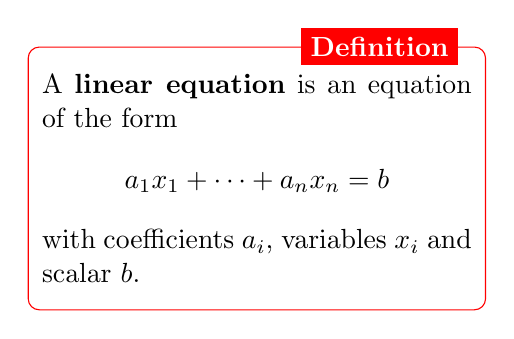
\begin{tikzpicture}
\node [rounded-box] (box){\begin{minipage}{0.45\textwidth}
    A \textbf{linear equation} is an equation of the form
    $$a_1 x_1 + \dots + a_n x_n = b$$
    with coefficients $a_i$, variables $x_i$ and scalar $b$.
\end{minipage}};
\node[rounded-box-title, left=10pt] at (box.north east) {Definition};
\end{tikzpicture}

\switchcolumn

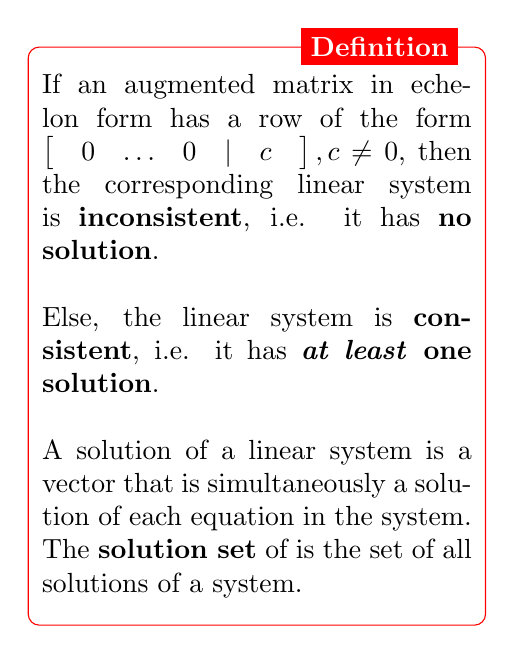
\begin{tikzpicture}
\node [rounded-box] (box){\begin{minipage}{0.45\textwidth}
    If an augmented matrix in echelon form has a row of the form $\begin{bmatrix}& 0 & \dots & 0 & | & c &\end{bmatrix}, c \neq 0$, then the corresponding linear system is \textbf{inconsistent}, i.e. it has \textbf{no solution}. \\

    Else, the linear system is \textbf{consistent}, i.e. it has \textbf{\textit{at least} one solution}. \\

    A solution of a linear system is a vector that is simultaneously a solution of each equation in the system. The \textbf{solution set} of is the set of all solutions of a system.
\end{minipage}};
\node[rounded-box-title, left=10pt] at (box.north east) {Definition};
\end{tikzpicture}

\textbf{Example}: Is $A\mathbf{x}=\mathbf{0}$ consistent? Yes, $\mathbf{x}=\mathbf{0}$ is always a solution, regardless of $A$. Therefore, $A\mathbf{x}=\mathbf{0}$ has either one or infinitely many solutions.

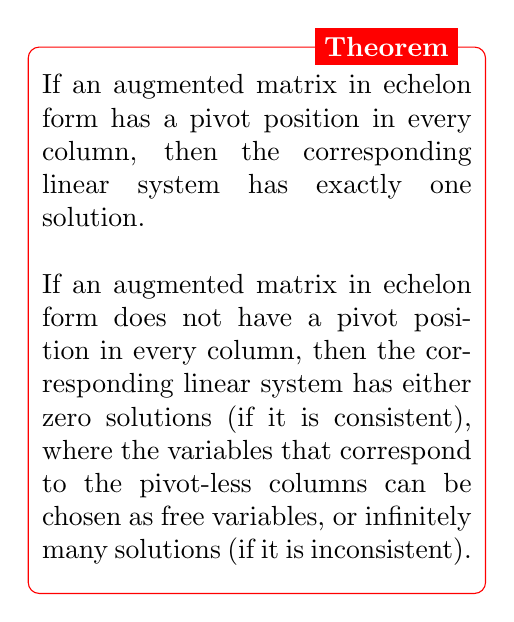
\begin{tikzpicture}
\node [rounded-box] (box){\begin{minipage}{0.45\textwidth}
    If an augmented matrix in echelon form has a pivot position in every column, then the corresponding linear system has exactly one solution. \\

    If an augmented matrix in echelon form does not have a pivot position in every column, then the corresponding linear system has either zero solutions (if it is consistent), where the variables that correspond to the pivot-less columns can be chosen as free variables, or infinitely many solutions (if it is inconsistent).
\end{minipage}};
\node[rounded-box-title, left=10pt] at (box.north east) {Theorem};
\end{tikzpicture}

\textbf{Example}: Suppose the augmented matrix corresponding to a consistent system is in echelon form. Then the variables corresponding to a pivot-less column can be chosen as free variables, in \textbf{parametric vector form}:

$$
\begin{bmatrix}
    x_1 \\ x_2 \\ x_3
\end{bmatrix} = \begin{bmatrix}
    4 \\ 0 \\ 3
\end{bmatrix} + s \begin{bmatrix}
    -3 \\ 1 \\ 0
\end{bmatrix}, s \in \mathbb{R}
$$

\switchcolumn

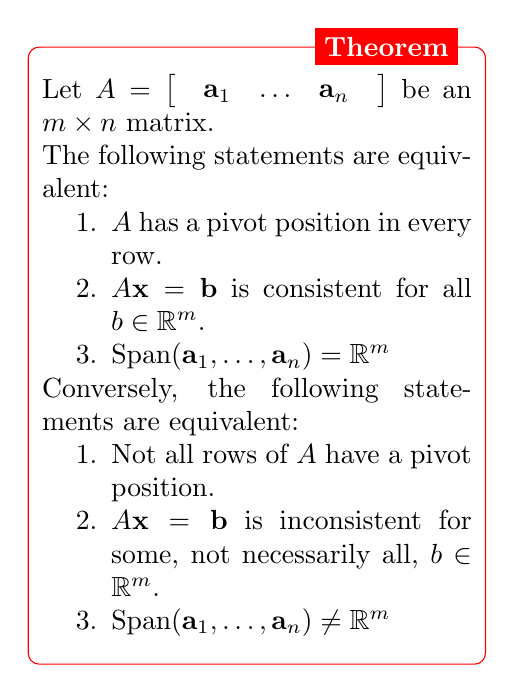
\begin{tikzpicture}
\node [rounded-box] (box){\begin{minipage}{0.45\textwidth}
    Let $A = \begin{bmatrix}& \mathbf{a}_1 & \dots & \mathbf{a}_n & \end{bmatrix}$ be an $m \times n$ matrix. \\
    The following statements are equivalent:
    \begin{enumerate}
        \item $A$ has a pivot position in every row.
        \item $A \mathbf{x} = \mathbf{b}$ is consistent for all $b \in \mathbb{R}^m$.
        \item $\text{Span}({\mathbf{a}_1, \dots, \mathbf{a}_n}) = \mathbb{R}^m$
    \end{enumerate}
    Conversely, the following statements are equivalent:
    \begin{enumerate}
        \item Not all rows of $A$ have a pivot position.
        \item $A \mathbf{x} = \mathbf{b}$ is inconsistent for some, not necessarily all, $b\in \mathbb{R}^m$.
        \item $\text{Span}({\mathbf{a}_1, \dots, \mathbf{a}_n}) \neq \mathbb{R}^m$
    \end{enumerate}
\end{minipage}};
\node[rounded-box-title, left=10pt] at (box.north east) {Theorem};
\end{tikzpicture}

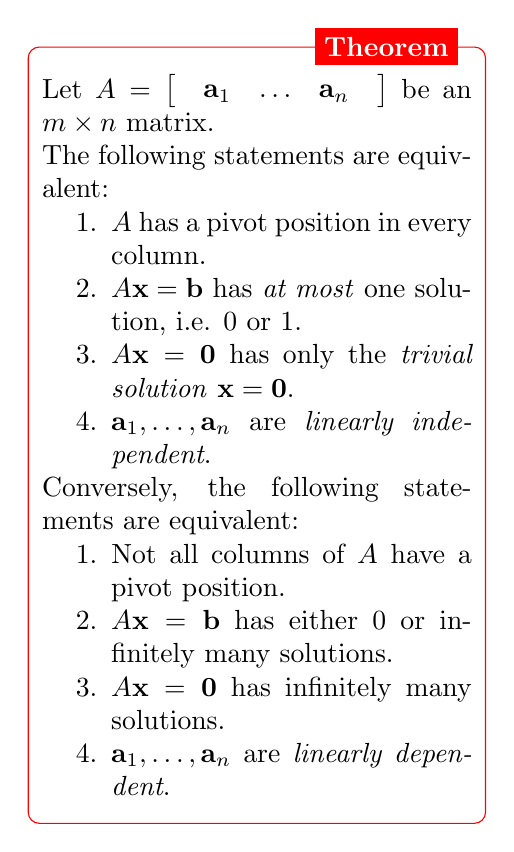
\begin{tikzpicture}
\node [rounded-box] (box){\begin{minipage}{0.45\textwidth}
    Let $A = \begin{bmatrix}& \mathbf{a}_1 & \dots & \mathbf{a}_n & \end{bmatrix}$ be an $m \times n$ matrix. \\
    The following statements are equivalent:
    \begin{enumerate}
        \item $A$ has a pivot position in every column.
        \item $A \mathbf{x} = \mathbf{b}$ has \textit{at most} one solution, i.e. $0$ or $1$.
        \item $A \mathbf{x} = \mathbf{0}$ has only the \textit{trivial solution} $\mathbf{x}=\mathbf{0}$.
        \item $\mathbf{a}_1, \dots, \mathbf{a}_n$ are \textit{linearly independent}.
    \end{enumerate}
    Conversely, the following statements are equivalent:
    \begin{enumerate}
        \item Not all columns of $A$ have a pivot position.
        \item $A \mathbf{x} = \mathbf{b}$ has either $0$ or infinitely many solutions.
        \item $A \mathbf{x} = \mathbf{0}$ has infinitely many solutions.
        \item $\mathbf{a}_1, \dots, \mathbf{a}_n$ are \textit{linearly dependent}.
    \end{enumerate}
\end{minipage}};
\node[rounded-box-title, left=10pt] at (box.north east) {Theorem};
\end{tikzpicture}

\switchcolumn

\textbf{Example}: This augmented matrix in echelon form does not have a pivot position in every row, i.e. it is inconsistent for some $\mathbf{\beta}$; but a pivot position in every column, so it has \textbf{either} $0$ - if $\beta_4 \neq 0$ - \textbf{or infinitely many} - if $\beta_4 = 0$ - \textbf{solutions}:

$$
\left[\begin{array}{ccc|c}
    1 & 2 & 4 & \beta_1 \\
    0 & 2 & 2 & \beta_2 \\
    0 & 0 & 4 & \beta_3 \\
    0 & 0 & 0 & \beta_4 \\
\end{array}\right]
$$

\switchcolumn

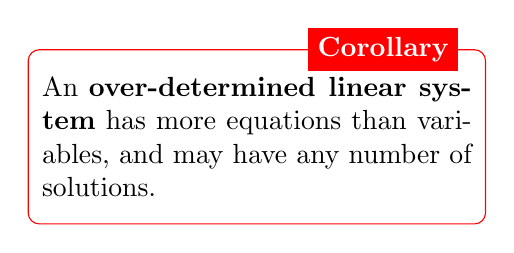
\begin{tikzpicture}
\node [rounded-box] (box){\begin{minipage}{0.45\textwidth}
    An \textbf{over-determined linear system} has more equations than variables, and may have any number of solutions.
\end{minipage}};
\node[rounded-box-title, left=10pt] at (box.north east) {Corollary};
\end{tikzpicture}

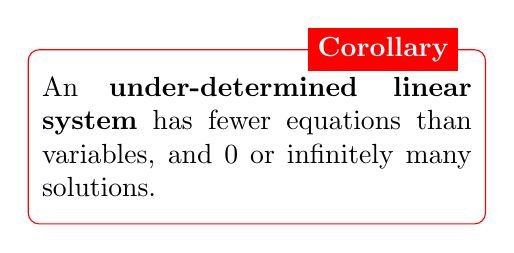
\begin{tikzpicture}
\node [rounded-box] (box){\begin{minipage}{0.45\textwidth}
    An \textbf{under-determined linear system} has fewer equations than variables, and $0$ or infinitely many solutions.
\end{minipage}};
\node[rounded-box-title, left=10pt] at (box.north east) {Corollary};
\end{tikzpicture}

Since each row has at most one pivot position and each column has at most one pivot position, there must be pivot-less columns. This means that if the system is consistent, there must be free variables. One solution is not possible.

\end{paracol}

\subsection{Geometric Interpretation of Linear Systems}

\begin{paracol}{2}

Systems of linear equations in two variables correspond to lines in $\mathbb{R}^2$. It is possible that they intersect in a point, are parallel, or do neither. Non-parallel lines that do not intersect are called skew lines.

Systems of linear equations in three variables correspond to planes in $\mathbb{R}^3$. It is possible that they intersect in a point, in a line, or neither (picture a water wheel).

\begin{center}
\begin{tabular}{c|c}
    \textbf{Intersection in} $\mathbf{R}^n$: & \textbf{Number of solutions}: \\
    \hline
    A line. & $\infty$ \\
    A point. & 1 \\
    None. & 0
\end{tabular}
\end{center}

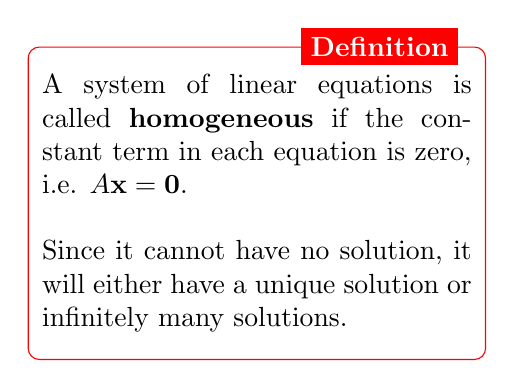
\begin{tikzpicture}
\node [rounded-box] (box){\begin{minipage}{0.45\textwidth}
    A system of linear equations is called \textbf{homogeneous} if the constant term in each equation is zero, i.e. $A \mathbf{x} = \mathbf{0}$. \\
    
    Since it cannot have no solution, it will either have a unique solution or infinitely many solutions.
\end{minipage}};
\node[rounded-box-title, left=10pt] at (box.north east) {Definition};
\end{tikzpicture}

\switchcolumn

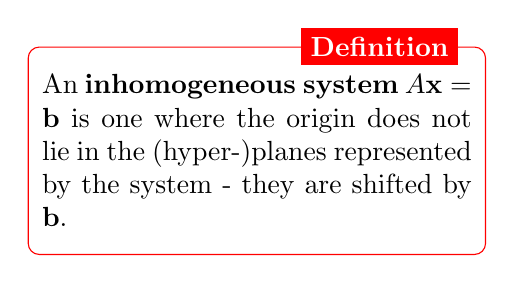
\begin{tikzpicture}
\node [rounded-box] (box){\begin{minipage}{0.45\textwidth}
    An \textbf{inhomogeneous system} $A \mathbf{x} = \mathbf{b}$ is one where the origin does not lie in the (hyper-)planes represented by the system - they are shifted by $\mathbf{b}$.
\end{minipage}};
\node[rounded-box-title, left=10pt] at (box.north east) {Definition};
\end{tikzpicture}

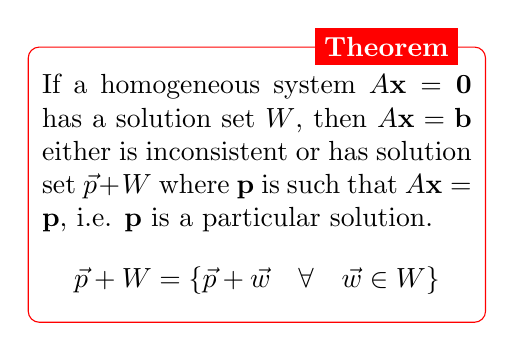
\begin{tikzpicture}
\node [rounded-box] (box){\begin{minipage}{0.45\textwidth}
    If a homogeneous system $A \mathbf{x} = \mathbf{0}$ has a solution set $W$, then $A \mathbf{x} = \mathbf{b}$ either is inconsistent or has solution set $\vec{p} + W$ where $\mathbf{p}$ is such that $A \mathbf{x} = \mathbf{p}$, i.e. $\mathbf{p}$ is a particular solution.
    $$\vec{p} + W = \{\vec{p} + \vec{w} \quad \forall \quad \vec{w} \in W\}$$
\end{minipage}};
\node[rounded-box-title, left=10pt] at (box.north east) {Theorem};
\end{tikzpicture}

That is, the solution set of a \textit{consistent} inhomogeneous linear system is parallel to the solution set of its corresponding homogeneous linear system.

\textbf{Example}: $A \mathbf{x} = \mathbf{b}$ has one solution, i.e. $|\{\mathbf{p} + W\}| = 1$. Then the size of the solution set of $A \mathbf{x} = \mathbf{0}$ is also $1$.

\end{paracol}

\subsection{Linear Independence}

\begin{paracol}{2}

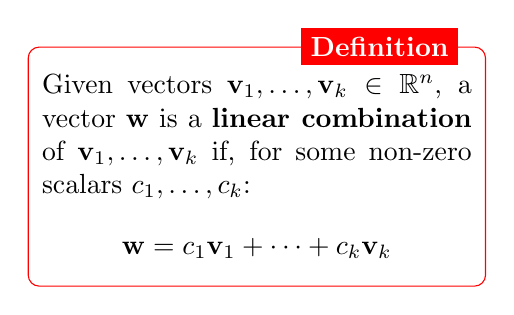
\begin{tikzpicture}
\node [rounded-box] (box){\begin{minipage}{0.45\textwidth}
    Given vectors $\mathbf{v}_1, \dots, \mathbf{v}_k \in \mathbb{R}^n$, a vector $\mathbf{w}$ is a \textbf{linear combination} of $\mathbf{v}_1, \dots, \mathbf{v}_k$ if, for some non-zero scalars $c_1, \dots, c_k$:
    $$\mathbf{w} = c_1 \mathbf{v}_1 + \dots + c_k \mathbf{v}_k$$
\end{minipage}};
\node[rounded-box-title, left=10pt] at (box.north east) {Definition};
\end{tikzpicture}

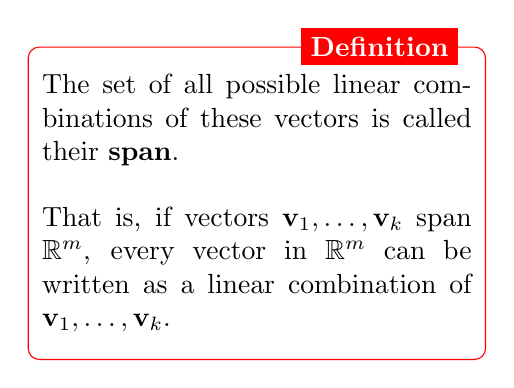
\begin{tikzpicture}
\node [rounded-box] (box){\begin{minipage}{0.45\textwidth}
    The set of all possible linear combinations of these vectors is called their \textbf{span}. \\

    That is, if vectors $\mathbf{v}_1, \dots, \mathbf{v}_k$ span $\mathbb{R}^m$, every vector in $\mathbb{R}^m$ can be written as a linear combination of $\mathbf{v}_1, \dots, \mathbf{v}_k$.
\end{minipage}};
\node[rounded-box-title, left=10pt] at (box.north east) {Definition};
\end{tikzpicture}

\textbf{Example}: $\text{Span}(\{\mathbf{u}, \dots, \mathbf{v}\})$ is the plane through $\mathbf{u}, \dots, \mathbf{v}$. \\

A set of vectors is \textbf{linearly dependent} if at least one of the vectors can be written as a linear combination of the others.

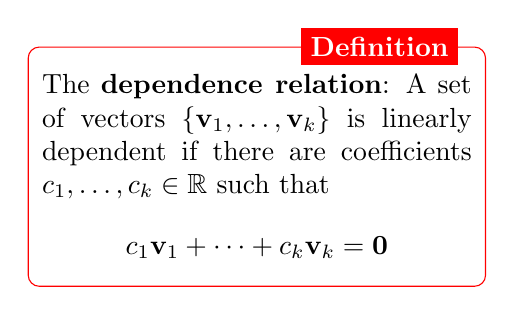
\begin{tikzpicture}
\node [rounded-box] (box){\begin{minipage}{0.45\textwidth}
    The \textbf{dependence relation}:
    A set of vectors $\{\mathbf{v}_1, \dots, \mathbf{v}_k\}$ is linearly dependent if there are coefficients $c_1, \dots, c_k \in \mathbb{R}$ such that
    $$c_1 \mathbf{v}_1 + \dots + c_k \mathbf{v}_k = \mathbf{0}$$
\end{minipage}};
\node[rounded-box-title, left=10pt] at (box.north east) {Definition};
\end{tikzpicture}

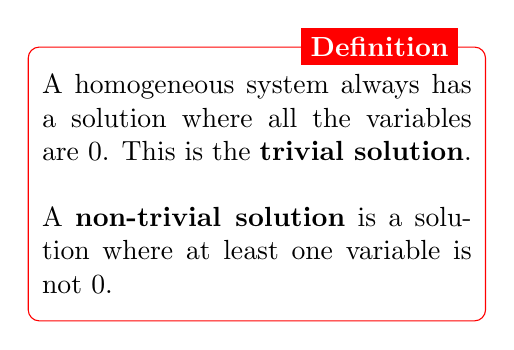
\begin{tikzpicture}
\node [rounded-box] (box){\begin{minipage}{0.45\textwidth}
    A homogeneous system always has a solution where all the variables are $0$. This is the \textbf{trivial solution}. \\

    A \textbf{non-trivial solution} is a solution where at least one variable is not $0$.
\end{minipage}};
\node[rounded-box-title, left=10pt] at (box.north east) {Definition};
\end{tikzpicture}

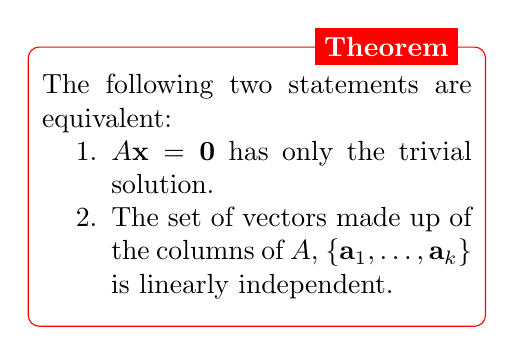
\begin{tikzpicture}
\node [rounded-box] (box){\begin{minipage}{0.45\textwidth}
    The following two statements are equivalent:
    \begin{enumerate}
        \item $A\mathbf{x} = \mathbf{0}$ has only the trivial solution.
        \item The set of vectors made up of the columns of $A$, $\{\mathbf{a}_1, \dots, \mathbf{a}_k\}$ is linearly independent.
    \end{enumerate}
\end{minipage}};
\node[rounded-box-title, left=10pt] at (box.north east) {Theorem};
\end{tikzpicture}

\switchcolumn

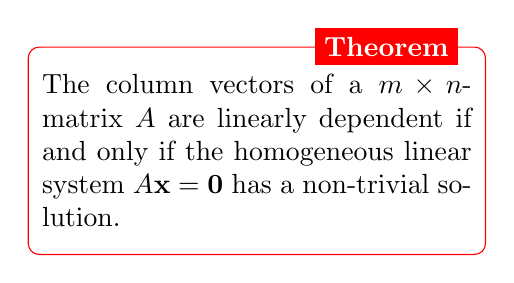
\begin{tikzpicture}
\node [rounded-box] (box){\begin{minipage}{0.45\textwidth}
    The column vectors of a $m \times n$-matrix $A$ are linearly dependent if and only if the homogeneous linear system $A \mathbf{x} = \mathbf{0}$ has a non-trivial solution.
\end{minipage}};
\node[rounded-box-title, left=10pt] at (box.north east) {Theorem};
\end{tikzpicture}

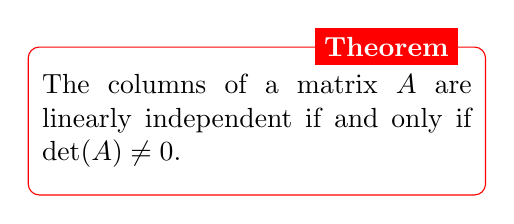
\begin{tikzpicture}
\node [rounded-box] (box){\begin{minipage}{0.45\textwidth}
    The columns of a matrix $A$ are linearly independent if and only if $\det(A) \neq 0$.
\end{minipage}};
\node[rounded-box-title, left=10pt] at (box.north east) {Theorem};
\end{tikzpicture}

Elementary row operations have a specific effect on the determinant of the matrix:

\begin{itemize}
    \item Swapping rows: This operation flips the sign of the determinant.
    \item Multiplying a row by a non-zero scalar: This operation multiplies the determinant by the same scalar.
    \item Adding a multiple of one row to another: This operation doesn't change the determinant itself.
\end{itemize}

If $\det(A) = 0$, then there exists a non-trivial solution to the system of linear equations represented by the rows of $A$.

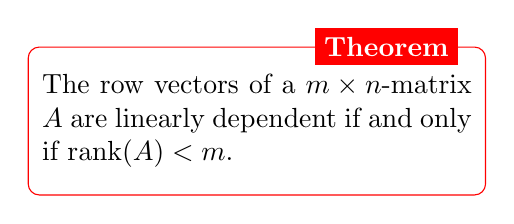
\begin{tikzpicture}
\node [rounded-box] (box){\begin{minipage}{0.45\textwidth}
    The row vectors of a $m \times n$-matrix $A$ are linearly dependent if and only if $\text{rank}(A) < m$.
\end{minipage}};
\node[rounded-box-title, left=10pt] at (box.north east) {Theorem};
\end{tikzpicture}

Thus, the rows of a matrix will be linearly dependent if elementary row operations can be used to crate a zero row.

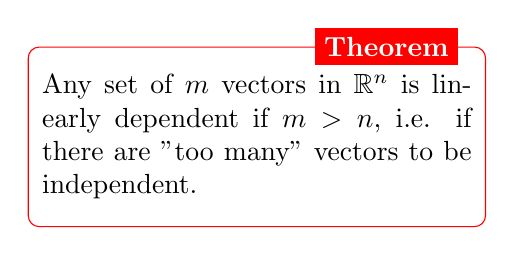
\begin{tikzpicture}
\node [rounded-box] (box){\begin{minipage}{0.45\textwidth}
    Any set of $m$ vectors in $\mathbb{R}^n$ is linearly dependent if $m > n$, i.e. if there are "too many" vectors to be independent.
    \end{minipage}};
\node[rounded-box-title, left=10pt] at (box.north east) {Theorem};
\end{tikzpicture}

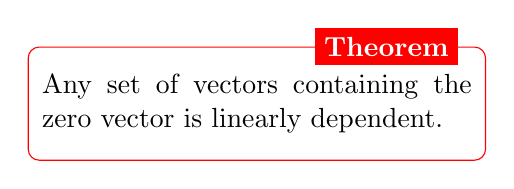
\begin{tikzpicture}
\node [rounded-box] (box){\begin{minipage}{0.45\textwidth}
    Any set of vectors containing the zero vector is linearly dependent.
\end{minipage}};
\node[rounded-box-title, left=10pt] at (box.north east) {Theorem};
\end{tikzpicture}

\end{paracol}
 \newpage
\section{Linear Subspaces}

\begin{paracol}{2}

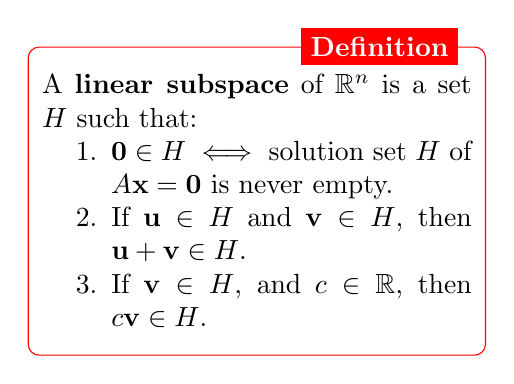
\begin{tikzpicture}
\node [rounded-box] (box){\begin{minipage}{0.45\textwidth}
    A \textbf{linear subspace} of $\mathbb{R}^n$ is a set $H$ such that:
    \begin{enumerate}
        \item $\mathbf{0} \in H \iff $ solution set $H$ of $A\mathbf{x}=\mathbf{0}$ is never empty.
        \item If $\mathbf{u} \in H$ and $\mathbf{v} \in H$, then $\mathbf{u} + \mathbf{v} \in H$.
        \item If $\mathbf{v} \in H$, and $c \in \mathbb{R}$, then $c\mathbf{v} \in H$.
    \end{enumerate}
\end{minipage}};
\node[rounded-box-title, left=10pt] at (box.north east) {Definition};
\end{tikzpicture}

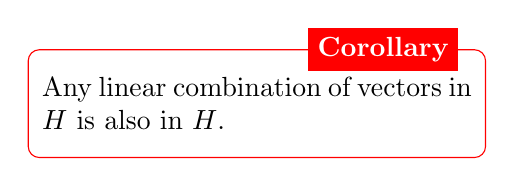
\begin{tikzpicture}
\node [rounded-box] (box){\begin{minipage}{0.45\textwidth}
    Any linear combination of vectors in $H$ is also in $H$.
\end{minipage}};
\node[rounded-box-title, left=10pt] at (box.north east) {Corollary};
\end{tikzpicture}

\switchcolumn

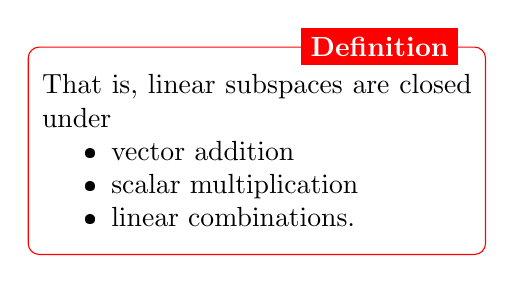
\begin{tikzpicture}
\node [rounded-box] (box){\begin{minipage}{0.45\textwidth}
    That is, linear subspaces are closed under
    \begin{itemize}
        \item vector addition
        \item scalar multiplication
        \item linear combinations.
    \end{itemize}
\end{minipage}};
\node[rounded-box-title, left=10pt] at (box.north east) {Definition};
\end{tikzpicture}

That is, you cannot get out of a linear subspace by means of any of these operations. \textbf{Example}: If vectors $\mathbf{v}_1, \dots, \mathbf{v}_k$ are in a subspace and $c_1, \dots, c_k$ are scalars, then the linear combination $c_1 \mathbf{v}_1 + \dots + c_k \mathbf{v}_k$ is in the subspace.

\end{paracol}

\textbf{Examples}: What is a subspace in $\mathbb{R}^n$?
\begin{itemize}
    \item The origin $\mathbf{0}$ by itself is the smallest possible linear subspace.
    \item Every line through the origin is a subspace.
    \item Every plane through the origin is a subspace - it is $\mathbb{R}^2$. (And every higher-dimensional hyperplane in $\mathbb{R}^n$.)
    \item Let $\mathbf{v}_1, \dots, \mathbf{v}_k \in \mathbb{R}^n$. Then $\text{Span}(\mathbf{v}_1, \dots, \mathbf{v}_k)$ is a subspace of $\mathbb{R}^n$.
    \item Any line, plane or hyperplane that does not pass through the origin is not a linear subspace.
    \item The first quadrant in $\mathbb{R}^2$, is not a linear subspace because $-\mathbf{v}$ would not be in the space, i.e. property 3 does not hold.
\end{itemize}

Two subspaces of a vector space may never be disjoint because by definition they must contain the zero vector.

\begin{paracol}{2}

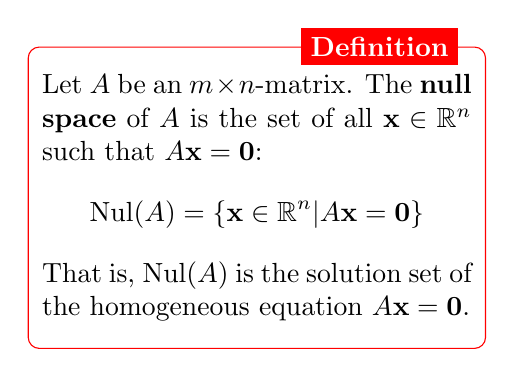
\begin{tikzpicture}
\node [rounded-box] (box){\begin{minipage}{0.45\textwidth}
    Let $A$ be an $m \times n$-matrix. The \textbf{null space} of $A$ is the set of all $\mathbf{x} \in \mathbb{R}^n$ such that $A\mathbf{x} = \mathbf{0}$:
    $$\text{Nul}(A) = \{\mathbf{x} \in \mathbb{R}^n | A\mathbf{x} = \mathbf{0} \}$$
    That is, $\text{Nul}(A)$ is the solution set of the homogeneous equation $A\mathbf{x}=\mathbf{0}$.
\end{minipage}};
\node[rounded-box-title, left=10pt] at (box.north east) {Definition};
\end{tikzpicture}

\textbf{Example}: Is $\mathbf{p} \in \text{Nul}(A)$? If $A\mathbf{p}=\mathbf{0}$, yes; else, no.

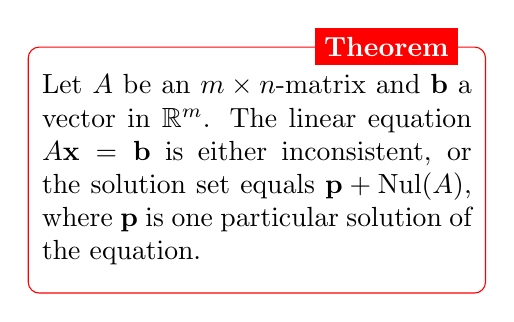
\begin{tikzpicture}
\node [rounded-box] (box){\begin{minipage}{0.45\textwidth}
    Let $A$ be an $m \times n$-matrix and $\mathbf{b}$ a vector in $\mathbb{R}^m$. The linear equation $A\mathbf{x}=\mathbf{b}$ is either inconsistent, or the solution set equals $\mathbf{p} + \text{Nul}(A)$, where $\mathbf{p}$ is one particular solution of the equation.
\end{minipage}};
\node[rounded-box-title, left=10pt] at (box.north east) {Theorem};
\end{tikzpicture}

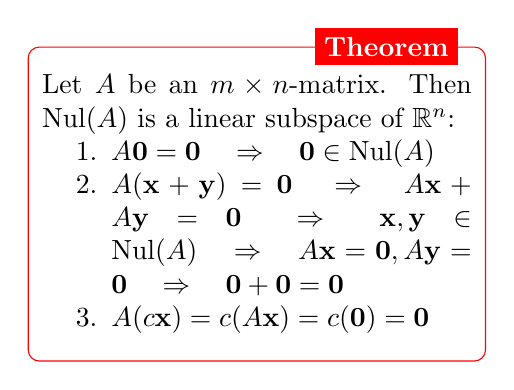
\begin{tikzpicture}
\node [rounded-box] (box){\begin{minipage}{0.45\textwidth}
    Let $A$ be an $m \times n$-matrix. Then $\text{Nul}(A)$ is a linear subspace of $\mathbb{R}^n$:
    \begin{enumerate}
        \item $A \mathbf{0} = \mathbf{0} \quad \Rightarrow \quad \mathbf{0} \in \text{Nul}(A)$
        \item $A(\mathbf{x} + \mathbf{y}) = \mathbf{0} \quad \Rightarrow \quad A\mathbf{x} + A\mathbf{y} = \mathbf{0} \quad \Rightarrow \quad \mathbf{x}, \mathbf{y} \in \text{Nul}(A) \quad \Rightarrow \quad A\mathbf{x}=\mathbf{0}, A\mathbf{y}=\mathbf{0} \quad \Rightarrow \quad \mathbf{0} + \mathbf{0} = \mathbf{0}$
        \item $A(c\mathbf{x}) = c(A\mathbf{x}) = c(\mathbf{0}) = \mathbf{0}$
    \end{enumerate}
\end{minipage}};
\node[rounded-box-title, left=10pt] at (box.north east) {Theorem};
\end{tikzpicture}

\switchcolumn

\begin{tikzpicture}
\node [rounded-box] (box){\begin{minipage}{0.45\textwidth}
    Let $A$ be an $m \times n$ matrix. The \textbf{row space} of $A$ is the subspace $\text{Row}(A)$ of $\mathbb{R}^n$ spanned by the rows of $A$.
\end{minipage}};
\node[rounded-box-title, left=10pt] at (box.north east) {Definition};
\end{tikzpicture}

\begin{tikzpicture}
\node [rounded-box] (box){\begin{minipage}{0.45\textwidth}
    Let $B$ be any matrix that is row-equivalent to a matrix $A$. Then $\text{Row}(B) = \text{Row}(A)$.
\end{minipage}};
\node[rounded-box-title, left=10pt] at (box.north east) {Theorem};
\end{tikzpicture}

\begin{tikzpicture}
\node [rounded-box] (box){\begin{minipage}{0.45\textwidth}
    Let $A$ be an $m \times n$ matrix. The \textbf{column space} of $A$ is the subspace $\text{Col}(A)$ of $\mathbb{R}^m$ spanned by the columns of $A$.
\end{minipage}};
\node[rounded-box-title, left=10pt] at (box.north east) {Definition};
\end{tikzpicture}

That is, the column space is the set of all possible outcomes of the multiplication $A\mathbf{x}$ - the set of all linear combinations of the columns of $A$:

$$\text{Col}(A) = \{ x_1 \mathbf{a}_1 + \dots + x_n \mathbf{a}_n \text{ for } x_1, \dots, x_n \in \mathbb{R} \}$$

\begin{tikzpicture}
\node [rounded-box] (box){\begin{minipage}{0.45\textwidth}
    It follows that $\mathbf{b} \in \text{Col}(A)$ iff $A \mathbf{x} = \mathbf{b}$ is consistent:
    $$\text{Col}(A) = \{ \mathbf{b} \in \mathbb{R}^m \text{ for which } A\mathbf{x}=\mathbf{b} \text{ is consistent} \}$$
\end{minipage}};
\node[rounded-box-title, left=10pt] at (box.north east) {Corollary};
\end{tikzpicture}

\end{paracol}

\textbf{Example}: Null Space

\vspace{-20pt}

$$
\left[\begin{array}{cccc|c}
    1 & 2 & -5 & -1 & 0 \\
    2 & -1 & 0 & 3 & 0
\end{array}\right]
\qquad \rightarrow \qquad
\mathbf{x} = s \begin{bmatrix}
    1 \\ 2 \\ 1 \\ 0
\end{bmatrix} + t \begin{bmatrix}
    -1 \\ 1 \\ 0 \\ 1
\end{bmatrix}, \quad s, t \in \mathbb{R}
\qquad \rightarrow \qquad
\text{Nul}(A) = \Bigg\{ \begin{bmatrix}
    1 \\ 2 \\ 1 \\ 0
\end{bmatrix}, \begin{bmatrix}
    -1 \\ 1 \\ 0 \\ 1
\end{bmatrix} \Bigg\}
$$

\begin{tikzpicture}
\node [rounded-box] (box){\begin{minipage}{0.95\textwidth}
    The span of any set of vectors is a linear subspace.
    That is, given vectors $\mathbf{v}_1, \dots, \mathbf{v}_k \in \mathbb{R}^m$, $\text{Span}(\{ \mathbf{v}_1, \dots, \mathbf{v}_k \})$ is a linear subspace of $\mathbb{R}^m$: \\

    \begin{enumerate}
        \item $0 \mathbf{v}_1 + \dots + 0 \mathbf{v}_k = \mathbf{0} \Rightarrow \mathbf{0} \in \text{Span}(\{ \mathbf{v}_1, \dots, \mathbf{v}_k \})$
        \item $\mathbf{x} = c_1 \mathbf{v}_1 + \dots + c_k \mathbf{v}_k \in \text{Span}(\{ \mathbf{v}_1, \dots, \mathbf{v}_k \}), \mathbf{y} = d_1 \mathbf{v}_1 + \dots + d_k \mathbf{v}_k \in \text{Span}(\{ \mathbf{v}_1, \dots, \mathbf{v}_k \}) \Rightarrow \mathbf{x} + \mathbf{y} = (c_1 + d_1) \mathbf{v}_1 + \dots + (c_k + d_k) \mathbf{v}_k \Rightarrow \mathbf{x} + \mathbf{y} \in \text{Span}(\{ \mathbf{v}_1, \dots, \mathbf{v}_k \})$
        \item $c \mathbf{x} = (c \cdot c_1)\mathbf{v}_1 + \dots + (c \cdot)\mathbf{v}_k \Rightarrow c \mathbf{x} \in \text{Span}(\{ \mathbf{v}_1, \dots, \mathbf{v}_k \})$
    \end{enumerate}
\end{minipage}};
\node[rounded-box-title, left=10pt] at (box.north east) {Theorem};
\end{tikzpicture}

\newpage

\subsection{Basis}

\begin{paracol}{2}

In a linear subspace, you can add vectors and multiply them by scalars, just as in $\mathbb{R}^n$. This connection between a subspace and $\mathbb{R}^n$ can be made precise using the definition of a basis.

\begin{tikzpicture}
\node [rounded-box] (box){\begin{minipage}{0.45\textwidth}
    A set $\{\mathbf{v}_1, \dots, \mathbf{v}_k\} \in \mathbb{R}^n$ is a \textbf{basis} for subspace $H \in \mathbb{R}^n$ if:
    \begin{itemize}
        \item the set $\{\mathbf{v}_1, \dots, \mathbf{v}_k\}$ is linearly independent, and
        \item $H = \text{Span}(\{\mathbf{v}_1, \dots, \mathbf{v}_k\})$.
    \end{itemize}
\end{minipage}};
\node[rounded-box-title, left=10pt] at (box.north east) {Definition};
\end{tikzpicture}

\begin{itemize}
    \item A set of vectors is linearly independent if $A\mathbf{x} = \mathbf{0}$ has only the trivial solution $\mathbf{x} = \mathbf{0}$, i.e. pivot in every col.
    \item A set of vectors spans a subspace if $A \mathbf{x} = \mathbf{b}$ is consistent for all $\mathbf{b} \in \mathbb{R}^n$, i.e. if every row has a pivot position.
\end{itemize}

\begin{tikzpicture}
\node [rounded-box] (box){\begin{minipage}{0.45\textwidth}
    Let $B=\{\mathbf{b}_1, \dots, \mathbf{b}_k\}$ be a basis for subspace $H \in \mathbb{R}^n$. Then, for each vector $\mathbf{x} \in H$ there exists a \textbf{unique} set of scalars $c_1, \dots, c_k$ such that $\mathbf{x} = c_1 \mathbf{b}_1 + \dots + c_k \mathbf{b}_k$. \\

    That is, the $B$-coordinates of $\mathbf{x}$ are:
    $$[\mathbf{x}]_B = \begin{bmatrix}c_1 \\ \vdots \\ c_k\end{bmatrix}$$
\end{minipage}};
\node[rounded-box-title, left=10pt] at (box.north east) {Theorem};
\end{tikzpicture}

\begin{tikzpicture}
\node [rounded-box] (box){\begin{minipage}{0.45\textwidth}
    The $k^\text{th}$ standard unit vector $\mathbf{e}_k \in \mathbb{R}^n$ is the vector with component $k = 1$ and the other components equal to zero.
\end{minipage}};
\node[rounded-box-title, left=10pt] at (box.north east) {Definition};
\end{tikzpicture}

\switchcolumn

\begin{tikzpicture}
\node [rounded-box] (box){\begin{minipage}{0.45\textwidth}
    The set $\epsilon = \{ \mathbf{e}_1, \dots, \mathbf{e}_n \}$ of the standard unit vectors in $\mathbb{R}^n$ is a basis for $\mathbb{R}^n$ - the \textbf{standard basis}:
    $$\mathbf{x} = \begin{bmatrix}x_1 \\ \vdots \\ x_n\end{bmatrix} = x_1 \mathbf{e}_1 + \dots + x_n \mathbf{e}_n$$
\end{minipage}};
\node[rounded-box-title, left=10pt] at (box.north east) {Definition};
\end{tikzpicture}

The pivot columns in $RREF(A)$ are the standard unit vectors. They are linearly independent.

\begin{tikzpicture}
\node [rounded-box] (box){\begin{minipage}{0.45\textwidth}
    Let $A$ be an $m \times n$-matrix. The pivot columns of $A$ form a basis for $\text{Col}(A)$.
\end{minipage}};
\node[rounded-box-title, left=10pt] at (box.north east) {Theorem};
\end{tikzpicture}

\begin{tikzpicture}
\node [rounded-box] (box){\begin{minipage}{0.45\textwidth}
    Row operations preserve dependence relations between the columns of a matrix.
\end{minipage}};
\node[rounded-box-title, left=10pt] at (box.north east) {Theorem};
\end{tikzpicture}

\begin{tikzpicture}
\node [rounded-box] (box){\begin{minipage}{0.45\textwidth}
    Let $A$ be an $m \times n$-matrix. Suppose that the homogeneous equation $A\mathbf{x}=\mathbf{0}$ has $k$ free variables.
    Let $\mathbf{b}_i$ be the solution for which the $i^\text{th}$ free variable is $1$.
    Then $\{ \mathbf{b}_1, \dots, \mathbf{b}_k \}$ is a \textbf{basis for the null space} $\text{Nul}(A)$. \\

    That is, the solution vectors in parametric form span the null space. 
\end{minipage}};
\node[rounded-box-title, left=10pt] at (box.north east) {Theorem};
\end{tikzpicture}

\vspace{-5pt}

This theorem can be used to find a basis for any linear subspace given by homogeneous linear equations.

\end{paracol}

\vspace{-7.5pt}

\subsection{Dimension}

\begin{paracol}{2}

Dimension is the maximum number of independent directions.

That is, the dimension is equal to the number of vectors in a basis. But bases are not unique. However, all bases of a given subspace contain the same number of vectors:

\begin{tikzpicture}
\node [rounded-box] (box){\begin{minipage}{0.45\textwidth}
    All bases for a linear subspace of $\mathbb{R}^n$ contain the same number of vectors.
\end{minipage}};
\node[rounded-box-title, left=10pt] at (box.north east) {Theorem};
\end{tikzpicture}

Therefore, the idea of dimension works:

\begin{tikzpicture}
\node [rounded-box] (box){\begin{minipage}{0.45\textwidth}
    Let $H$ be a linear subspace of $\mathbb{R}^n$.
    Let $B=\{\mathbf{b}_1, \dots, \mathbf{b}_k\}$ be a basis for $H$.
    The \textbf{dimension} of $H$ is the number of vectors in $B$:
    $$\text{dim}(H) = k$$
\end{minipage}};
\node[rounded-box-title, left=10pt] at (box.north east) {Definition};
\end{tikzpicture}

\switchcolumn

\begin{tikzpicture}
\node [rounded-box] (box){\begin{minipage}{0.45\textwidth}
    Let $H$ be a linear subspace of $\mathbb{R}^n$ with $\text{dim}(H) = k$. Then the following statements hold:
    \begin{enumerate}
        \item There are at most $k$ distinct independent vectors in $H$.
        \item At least $k$ vectors are needed to span $H$.
        \item Vectors in $H$ can be described with $k$ coordinates.
    \end{enumerate}
\end{minipage}};
\node[rounded-box-title, left=10pt] at (box.north east) {Theorem};
\end{tikzpicture}

\begin{tikzpicture}
\node [rounded-box] (box){\begin{minipage}{0.45\textwidth}
    Let $H$ be a linear subspace of $\mathbb{R}^n$ with $\text{dim}(H)=k$.
    Let $S=\{\mathbf{v}_1, \dots, \mathbf{v}_k \}$ be a set of vectors in $H$. \\
    
    If set $S$ is linearly independent, then $S$ spans $H$. \\
    
    Hence it is a basis.
\end{minipage}};
\node[rounded-box-title, left=10pt] at (box.north east) {The Basis Theorem};
\end{tikzpicture}

NB: The vectors \textit{must} be in $H$ for the theorem to hold!

\end{paracol}

\vspace{-7.5pt}

\subsection{Rank}

\begin{paracol}{2}

\begin{tikzpicture}
\node [rounded-box] (box){\begin{minipage}{0.45\textwidth}
    The \textbf{column space} of a matrix $A$ is made up of the columns that have a pivot position.
\end{minipage}};
\node[rounded-box-title, left=10pt] at (box.north east) {Definition};
\end{tikzpicture}

\vspace{-2.5pt}

\begin{tikzpicture}
\node [rounded-box] (box){\begin{minipage}{0.45\textwidth}
    The \textbf{rank} of a matrix $A$ is the dimension of the column space of $A$:
    $$\text{rank}(A) = \text{dim}(\text{Col}(A) = \text{dim}(\text{Row}(A))$$
\end{minipage}};
\node[rounded-box-title, left=10pt] at (box.north east) {Theorem};
\end{tikzpicture}

\switchcolumn

\begin{tikzpicture}
\node [rounded-box] (box){\begin{minipage}{0.45\textwidth}
    The \textbf{null space} of a matrix $A$ is made up of the columns that do not have a pivot position, i.e. the number of free variables of equation $A\mathbf{x}=\mathbf{0}$.
\end{minipage}};
\node[rounded-box-title, left=10pt] at (box.north east) {Definition};
\end{tikzpicture}

\vspace{-5pt}

\begin{tikzpicture}
\node [rounded-box] (box){\begin{minipage}{0.45\textwidth}
    The \textbf{nullity} of a matrix $A$ is the dimension of the null space of $A$:
    $$\text{nullity}(A) = \text{dim}(\text{Nul}(A))$$
\end{minipage}};
\node[rounded-box-title, left=10pt] at (box.north east) {Theorem};
\end{tikzpicture}

\switchcolumn

\begin{tikzpicture}
\node [rounded-box] (box){\begin{minipage}{0.45\textwidth}
    For a consistent system of linear equations with coefficient matrix $A$:
    
    \begin{itemize}
        \item $\text{rank}(A)$ is the \textit{effective} number of equations.
        \item $\text{nullity}(A)$ is the number of free variables.
    \end{itemize}
\end{minipage}};
\node[rounded-box-title, left=10pt] at (box.north east) {Theorem};
\end{tikzpicture}

The number of free variables (/columns) equals the total number of variables (/columns) minus the effective number of equations (/rows):

\begin{tikzpicture}
\node [rounded-box] (box){\begin{minipage}{0.45\textwidth}
    Let $A$ be a matrix with $n$ columns. Then
    $$\text{rank}(A) + \text{nullity}(A) = n$$
\end{minipage}};
\node[rounded-box-title, left=10pt] at (box.north east) {Rank Theorem};
\end{tikzpicture}

\switchcolumn

The effective set of equations for any linear system can be found by putting the system in echelon form.

\begin{tikzpicture}
\node [rounded-box] (box){\begin{minipage}{0.45\textwidth}
    Let $A$ be an $m \times n$-matrix with $k$ pivot positions. Then
    \begin{align*}
        \text{rank}(A) = \text{dim}(\text{Col}(A)) & = k & (k \text{ pivot positions}) \\
        \text{nullity}(A) = \text{dim}(\text{Nul}(A)) & = n-k & (n-k \text{ free variables})
    \end{align*}
\end{minipage}};
\node[rounded-box-title, left=10pt] at (box.north east) {Theorem};
\end{tikzpicture}

\vspace{10pt}

\begin{tikzpicture}
\node [rounded-box] (box){\begin{minipage}{0.45\textwidth}
    For any matrix $A$,

    $$\text{rank}(A^T) = \text{rank}(A)$$
\end{minipage}};
\node[rounded-box-title, left=10pt] at (box.north east) {Theorem};
\end{tikzpicture}

\end{paracol}

\section{Orthogonality}

\subsection{Orthogonal Sets}

\begin{paracol}{2}

\begin{tikzpicture}
\node [rounded-box] (box){\begin{minipage}{0.45\textwidth}
    A set $\{\mathbf{v}_1, \dots, \mathbf{v}_k\}$ in $\mathbb{R}^n$ is an \textbf{orthogonal set} if all distinct vectors in the set are pairwise orthogonal:
    
    $$\mathbf{v}_i \cdot \mathbf{v}_j = 0 \text{ for } i \neq j$$
\end{minipage}};
\node[rounded-box-title, left=10pt] at (box.north east) {Definition};
\end{tikzpicture}

\begin{tikzpicture}
\node [rounded-box] (box){\begin{minipage}{0.45\textwidth}
    A set of vectors in $\mathbb{R}^n$ is an \textbf{orthonormal set} if it is an orthogonal set of unit vectors:

    $$||\mathbf{v}_i|| = 1 \text{ for all } i$$
\end{minipage}};
\node[rounded-box-title, left=10pt] at (box.north east) {Definition};
\end{tikzpicture}

\textbf{Example}: Orthonormal set from an orthogonal set

$$
S = \{ \mathbf{u}, \mathbf{v}, \mathbf{w} \} \Rightarrow \tilde{S} = \{ \frac{1}{||\mathbf{u}||}\mathbf{u}, \frac{1}{||\mathbf{v}||}\mathbf{v}, \frac{1}{||\mathbf{w}||}\mathbf{w} \}
$$

\begin{tikzpicture}
\node [rounded-box] (box){\begin{minipage}{0.45\textwidth}
    If $S = \{\mathbf{v}_1, \dots, \mathbf{v}_k\}$ is an orthogonal set of non-zero vectors in $\mathbb{R}^n$, then $S$ is linearly independent.
\end{minipage}};
\node[rounded-box-title, left=10pt] at (box.north east) {Theorem};
\end{tikzpicture}

\begin{tikzpicture}
\node [rounded-box] (box){\begin{minipage}{0.45\textwidth}
    Let $\{\mathbf{v}_1, \dots, \mathbf{v}_k\}$ be an orthogonal basis for a subspace $W$ of $\mathbb{R}^n$ and let $\mathbf{w}$ be any vector in $W$.
    Then the unique scalars $c_1, c_2, \dots, c_k$ such that $\mathbf{w} = c_1 \mathbf{v}_1 + c_2 \mathbf{v}_2 + \dots + c_k \mathbf{v}_k$ are given by

    $$c_i = \frac{\mathbf{w} \cdot \mathbf{v}_i}{\mathbf{v}_i \cdot \mathbf{v}_i}$$

    and this representation is unique.
\end{minipage}};
\node[rounded-box-title, left=10pt] at (box.north east) {Theorem};
\end{tikzpicture}

\textbf{Example}: How to use orthogonality to find coordinates:

$$
S = \{ \mathbf{v}_1, \mathbf{v}_2, \mathbf{v}_3 \} = \{ \begin{bmatrix} 1 \\ 3 \\ -2 \end{bmatrix}, \begin{bmatrix} 2 \\ 0 \\ 1 \end{bmatrix}, \begin{bmatrix} -3 \\ 5 \\ 6 \end{bmatrix} \}, \mathbf{x} = \begin{bmatrix} 1 \\ 2 \\ 0 \end{bmatrix}
$$

$$
\mathbf{x} = c_1 \mathbf{v}_1 + c_2 \mathbf{v}_2 + c_3 \mathbf{v}_3
$$

\vspace{-10pt}

$$
\begin{cases}
    \mathbf{x} \cdot \mathbf{v}_1 = c_1 \mathbf{v}_1 \cdot \mathbf{v}_1 + c_2 \mathbf{v}_1 \cdot \mathbf{v}_2 + c_3 \mathbf{v}_1 \cdot \mathbf{v}_3 \\
    \mathbf{x} \cdot \mathbf{v}_2 = c_1 \mathbf{v}_2 \cdot \mathbf{v}_1 + c_2 \mathbf{v}_2 \cdot \mathbf{v}_2 + c_3 \mathbf{v}_2 \cdot \mathbf{v}_3 \\
    \mathbf{x} \cdot \mathbf{v}_3 = c_1 \mathbf{v}_3 \cdot \mathbf{v}_1 + c_2 \mathbf{v}_3 \cdot \mathbf{v}_2 + c_3 \mathbf{v}_3 \cdot \mathbf{v}_3
\end{cases}
$$

\switchcolumn

\begin{align*}
\begin{cases}
    c_1 = \frac{\mathbf{x} \cdot \mathbf{v}_1}{\mathbf{v}_1 \cdot \mathbf{v}_1} & (\text{since } \mathbf{v}_1 \cdot \mathbf{v}_2 = \mathbf{v}_1 \cdot \mathbf{v}_3 = 0) \\
    c_2 = \frac{\mathbf{x} \cdot \mathbf{v}_2}{\mathbf{v}_2 \cdot \mathbf{v}_2} & (\text{since } \mathbf{v}_2 \cdot \mathbf{v}_1 = \mathbf{v}_2 \cdot \mathbf{v}_3 = 0) \\
    c_3 = \frac{\mathbf{x} \cdot \mathbf{v}_3}{\mathbf{v}_3 \cdot \mathbf{v}_3} & (\text{since } \mathbf{v}_3 \cdot \mathbf{v}_1 = \mathbf{v}_3 \cdot \mathbf{v}_2 = 0)
\end{cases}
\end{align*}

\begin{tikzpicture}
\node [rounded-box] (box){\begin{minipage}{0.45\textwidth}
    An \textbf{orthogonal basis} for a subspace $W$ of $\mathbb{R}^n$ is a basis of $W$ that is an orthogonal set.
\end{minipage}};
\node[rounded-box-title, left=10pt] at (box.north east) {Definition};
\end{tikzpicture}

\begin{tikzpicture}
\node [rounded-box] (box){\begin{minipage}{0.45\textwidth}
    Let $H$ be a linear subspace of $\mathbb{R}^n$, and $B = \{\mathbf{b}_1, \dots, \mathbf{b}_k\}$ an orthogonal basis for $H$. Let $\mathbf{x}$ be a vector in $H$. \\
    
    Then the coordinates of $\mathbf{x}$ with respect to $B$ are given by the orthogonal projection of $\mathbf{x}$ onto each $\mathbf{b}_i$:
    $$\mathbf{x} = (\frac{\mathbf{x} \cdot \mathbf{b}_1}{\mathbf{b}_1 \cdot \mathbf{b}_1})\mathbf{b}_1 + \dots + (\frac{\mathbf{x} \cdot \mathbf{b}_k}{\mathbf{b}_k \cdot \mathbf{b}_k})\mathbf{b}_k$$
\end{minipage}};
\node[rounded-box-title, left=10pt] at (box.north east) {Theorem};
\end{tikzpicture}

\begin{tikzpicture}
\node [rounded-box] (box){\begin{minipage}{0.45\textwidth}
    If $B$ is an \textbf{orthonormal basis}, then the coordinates are given by the dot product:
    $$\mathbf{x} = (\mathbf{x} \cdot \mathbf{b}_1) \mathbf{b}_1 + \dots + (\mathbf{x} \cdot \mathbf{b}_k) \mathbf{b}_k$$
\end{minipage}};
\node[rounded-box-title, left=10pt] at (box.north east) {Theorem};
\end{tikzpicture}

\textbf{Example}: A property of the standard basis in $\mathbb{R}^n$ is that each standard basis vector is a unit vector.

\begin{tikzpicture}
\node [rounded-box] (box){\begin{minipage}{0.45\textwidth}
    The columns of an $m \times n$ matrix $Q$ form an orthonormal set if and only if $Q^T Q = I_n$.
\end{minipage}};
\node[rounded-box-title, left=10pt] at (box.north east) {Theorem};
\end{tikzpicture}

\begin{tikzpicture}
\node [rounded-box] (box){\begin{minipage}{0.45\textwidth}
    A square matrix whose rows and columns each form an orthonormal set is called an \textbf{orthogonal matrix}.
\end{minipage}};
\node[rounded-box-title, left=10pt] at (box.north east) {Definition};
\end{tikzpicture}

\begin{tikzpicture}
\node [rounded-box] (box){\begin{minipage}{0.45\textwidth}
    A square matrix is orthogonal if and only if $Q^{-1} = Q^T$.
\end{minipage}};
\node[rounded-box-title, left=10pt] at (box.north east) {Theorem};
\end{tikzpicture}

\begin{tikzpicture}
\node [rounded-box] (box){\begin{minipage}{0.45\textwidth}
    If two square matrices $Q_1, Q_2$ are orthogonal, then so is $Q_1 Q_2$.
\end{minipage}};
\node[rounded-box-title, left=10pt] at (box.north east) {Theorem};
\end{tikzpicture}

\switchcolumn

\begin{tikzpicture}
\node [rounded-box] (box){\begin{minipage}{0.45\textwidth}
    Let $Q$ be an orthogonal matrix. Then \\

    \begin{enumerate}
        \item $|| Q \mathbf{x} || = || \mathbf{x} ||$ for every $\mathbf{x} \in \mathbb{R}^n$
        \item $Q \mathbf{x} \cdot Q \mathbf{y} = \mathbf{x} \cdot \mathbf{y}$ for every $\mathbf{x}, \mathbf{y} \in \mathbb{R}^n$
    \end{enumerate}
\end{minipage}};
\node[rounded-box-title, left=10pt] at (box.north east) {Theorem};
\end{tikzpicture}

\switchcolumn

\begin{tikzpicture}
\node [rounded-box] (box){\begin{minipage}{0.45\textwidth}
    Let $Q$ be an orthogonal matrix. Then

    \begin{enumerate}
        \item $Q^{-1}$ is orthogonal
        \item $\det(Q) = \pm 1$
        \item If $\lambda$ is an eigenvalue of $Q$, then $| \lambda | = 1$.
    \end{enumerate}
\end{minipage}};
\node[rounded-box-title, left=10pt] at (box.north east) {Theorem};
\end{tikzpicture}

\end{paracol}

\subsection{Orthogonal Complements}

Orthogonally decomposing a vector with respect to a linear subspace $H$ comes down to "splitting" the vector into a component in $H$ and a component in the orthogonal of $H$.

\begin{paracol}{2}

\begin{tikzpicture}
\node [rounded-box] (box){\begin{minipage}{0.45\textwidth}
    A vector $\mathbf{x}$ is orthogonal to a linear subspace $H$ or $\mathbb{R}^n$ if it is orthogonal to all vectors in $H$. That is: $\mathbf{v} \cdot \mathbf{x} = 0$ for all $\mathbf{x}$ in $H$.
\end{minipage}};
\node[rounded-box-title, left=10pt] at (box.north east) {Definition};
\end{tikzpicture}

\switchcolumn

\begin{tikzpicture}
\node [rounded-box] (box){\begin{minipage}{0.45\textwidth}
    The set of all vectors orthogonal to $H$ is the \textbf{orthogonal complement} of $H$, denoted $H^\perp$. That is,

    $H^\perp = \{ \mathbf{v} \in \mathbb{R}^n : \mathbf{v} \cdot \mathbf{x} = 0 \quad \forall \quad \mathbf{x} \in H \}$
\end{minipage}};
\node[rounded-box-title, left=10pt] at (box.north east) {Definition};
\end{tikzpicture}

\end{paracol}

\begin{tikzpicture}
\node [rounded-box] (box){\begin{minipage}{0.975\textwidth}
    Let $W$ be a subspace of $\mathbb{R}^n$. If $W = \text{Span}(\mathbf{w}_1, \dots, \mathbf{w}_k)$, then $\mathbf{v} \in W^\perp$ if and only if $\mathbf{v} \cdot \mathbf{w}_i = 0$ for all $i = 1, \dots, k$.
\end{minipage}};
\node[rounded-box-title, left=10pt] at (box.north east) {Theorem};
\end{tikzpicture}

\textbf{Example}: The orthogonal complement of $\mathbb{R}^n$ is the zero space - $\mathbf{0}$ is the only vector orthogonal to every vector in $\mathbb{R}^n$.

\begin{paracol}{2}

\begin{tikzpicture}
\node [rounded-box] (box){\begin{minipage}{0.45\textwidth}
    Let $A$ be an $m \times n$ matrix. Then
    $$( \text{Row}(A) )^\perp = \text{Nul}(A), \qquad ( \text{Nul}(A) )^\perp = \text{Row}(A)$$
    $$( \text{Col}(A) )^\perp = \text{Nul}(A^T), \qquad ( \text{Nul}(A) )^\perp = \text{Col}(A^T)$$
\end{minipage}};
\node[rounded-box-title, left=10pt] at (box.north east) {Theorem};
\end{tikzpicture}

\switchcolumn

\begin{tikzpicture}
\node [rounded-box] (box){\begin{minipage}{0.45\textwidth}
    The $m \times n$ matrix $A$ defines a linear transformation from $\mathbb{R}^n$ to $\mathbb{R}^m$

    \begin{itemize}
        \item whose range is $\text{Col}(A)$, and
        \item which sends $\text{Nul}(A)$ to $0$ in $\mathbb{R}^n$.
    \end{itemize}
\end{minipage}};
\node[rounded-box-title, left=10pt] at (box.north east) {Theorem};
\end{tikzpicture}

\end{paracol}

\textbf{Proof}: Suppose that $\mathbf{x} \in \text{Nul}(A^T)$, that is, $A^T \mathbf{x} = \mathbf{0}$. This means that $\mathbf{x}$ is orthogonal to each row of $A^T$ and hence to the span of the rows of $A^T$. But the rows of $A^T$ are the columns of $A$. This means that $\mathbf{x}$ is orthogonal to $\text{Col}(A)$.

\begin{paracol}{2}

\begin{tikzpicture}
\node [rounded-box] (box){\begin{minipage}{0.45\textwidth}
    Let $H = Span \{\mathbf{v}_1, \dots, \mathbf{v}_k\}$ be a linear subspace of $\mathbb{R}^n$. Then
    $$H^\perp = \{ \mathbf{x} \in \mathbb{R}^3 \mid \mathbf{v}_1 \cdot \mathbf{x} = 0, \mathbf{v}_2 \cdot \mathbf{x} = 0, \dots, \mathbf{v}_k \cdot \mathbf{x} = 0 \}$$

    That is,

    \begin{enumerate}
        \item $H^\perp$ is the solution set, i.e. the \textbf{null space}, of the homogeneous system of equations $A \mathbf{x} = \mathbf{0}$, and
        \item the vectors $\mathbf{v}_1, \dots, \mathbf{v}_k$ make up the row space of the matrix $A$.
    \end{enumerate}
\end{minipage}};
\node[rounded-box-title, left=10pt] at (box.north east) {Theorem};
\end{tikzpicture}

\switchcolumn

\begin{tikzpicture}
\node [rounded-box] (box){\begin{minipage}{0.45\textwidth}
    Let $H$ be a linear subspace of $\mathbb{R}^n$. Then \\

    \begin{enumerate}
        \item $(H^\perp)^\perp = H$.
        \item $dim(H) + dim(H^\perp) = n$ \\

        \item $H^\perp$ is a linear subspace of $\mathbb{R}^n$. (This follows from the fact that it is the solution set of a homogeneous system of equations.)
        \item The only vector that is both in $H$ and $H^\perp$ is the zero vector: $H \cap H^\perp = \{ \mathbf{0} \}$
    \end{enumerate}
\end{minipage}};
\node[rounded-box-title, left=10pt] at (box.north east) {Theorem};
\end{tikzpicture}

\end{paracol}

\textbf{Example}:

Let $W = \text{Span} \Bigg\{ \begin{pmatrix}
    -2, \\ 6 \\ -1 \\ -1
\end{pmatrix}, \begin{pmatrix}
    2 \\ -6 \\ -2 \\ 10
\end{pmatrix}, \begin{pmatrix}
    -4 \\ 12 \\ 4 \\ -20
\end{pmatrix} \Bigg\}$. The basis $\Bigg\{ \begin{pmatrix}
    3 \\ 1 \\ 0 \\ 0
\end{pmatrix}, \begin{pmatrix}
    -2 \\ 0 \\ 3 \\ 1
\end{pmatrix} \Bigg\}$ for $W^\perp$ can be found by solving the homogeneous system

$$
\begin{bmatrix}
    -2 & 6 & -1 & -1 & | & 0 \\
    2 & -6 & -2 & 10 & | & 0 \\
    -4 & 12 & 4 & -20 & | & 0 \\
\end{bmatrix} \sim \begin{bmatrix}
    1 & -3 & 0 & 2 & | & 0 \\
    0 & 0 & 1 & -3 & | & 0 \\
    0 & 0 & 0 & 0 & | & 0 \\
\end{bmatrix}
$$

\subsection{Orthogonal Projections}

\begin{tikzpicture}
\node [rounded-box] (box){\begin{minipage}{0.975\textwidth}
    If $\mathbf{u}, \mathbf{v}$ are vectors in $\mathbb{R}^n$ and $\mathbf{u} \neq \mathbf{0}$, then the projection of $\mathbf{v}$ onto $\mathbf{u}$ is a scalar multiple of $\mathbf{u}$ - the vector

    $$\text{Proj}_\mathbf{u}(\mathbf{v}) = \Big( \frac{\mathbf{u} \cdot \mathbf{v}}{\mathbf{u} \cdot \mathbf{u}} \Big) \mathbf{u}$$

    If $\mathbf{u}$ is a unit vector, then $\text{Proj}_\mathbf{u}(\mathbf{v}) = ( \mathbf{u} \cdot \mathbf{v} ) \mathbf{u}$.
\end{minipage}};
\node[rounded-box-title, left=10pt] at (box.north east) {Definition};
\end{tikzpicture}

\newpage

\begin{paracol}{2}

\begin{tikzpicture}
\node [rounded-box] (box){\begin{minipage}{0.45\textwidth}
    Let $W$ be a subspace of $\mathbb{R}^n$ and let $\{ \mathbf{u}_1, \dots, \mathbf{u}_k \}$ be an \textit{orthogonal} basis for $W$. For any vector $\mathbf{v} \in \mathbb{R}^n$, the orthogonal projection of $\mathbf{v}$ onto $W$ is

    \begin{align*}
        \text{Proj}_W(\mathbf{v}) & = \text{Proj}_W(\mathbf{u}_1) + \dots + \text{Proj}_W(\mathbf{u}_k) \\
        & = \Big( \frac{\mathbf{u}_1 \cdot \mathbf{v}}{\mathbf{u}_1 \cdot \mathbf{u}_1} \Big) \mathbf{u}_1 + \dots + \Big( \frac{\mathbf{u}_k \cdot \mathbf{v}}{\mathbf{u}_k \cdot \mathbf{u}_k} \Big) \mathbf{u}_k
    \end{align*}

    The component of $\mathbf{v}$ orthogonal to $W$ is the vector $\text{perp}_W(\mathbf{v}) = \mathbf{v} - \text{Proj}_W(\mathbf{v})$
\end{minipage}};
\node[rounded-box-title, left=10pt] at (box.north east) {Definition};
\end{tikzpicture}

\begin{tikzpicture}
\node [rounded-box] (box){\begin{minipage}{0.45\textwidth}
    Let $W$ be a subspace of $\mathbb{R}^n$ and let $\mathbf{v}$ be a vector in $\mathbb{R}^n$. Then there are unique vectors $\mathbf{w}$ in $W$ and $\mathbf{w}^\perp$ in $W^\perp$ such that
    $$\mathbf{v} = \mathbf{w} + \mathbf{w}^\perp$$
\end{minipage}};
\node[rounded-box-title, left=10pt] at (box.north east) {Orthogonal Decomposition Theorem};
\end{tikzpicture}

\begin{tikzpicture}
\node [rounded-box] (box){\begin{minipage}{0.45\textwidth}
    If $W$ is a subspace of $\mathbf{R}^n$, then $(W^\perp)^\perp = W$.
\end{minipage}};
\node[rounded-box-title, left=10pt] at (box.north east) {Theorem};
\end{tikzpicture}

\begin{tikzpicture}
\node [rounded-box] (box){\begin{minipage}{0.45\textwidth}
    If $W$ is a subspace of $\mathbb{R}^n$, then $\dim(W) + \dim(W^\perp) = n$.
\end{minipage}};
\node[rounded-box-title, left=10pt] at (box.north east) {Theorem};
\end{tikzpicture}

\begin{tikzpicture}
\node [rounded-box] (box){\begin{minipage}{0.45\textwidth}
    If $A$ is an $m \times n$ matrix, then

    \begin{itemize}
        \item $\text{rank}(A) + \text{nullity}(A) = n$
        \item $\text{rank}(A) + \text{nullity}(A^T) = m$
    \end{itemize}
\end{minipage}};
\node[rounded-box-title, left=10pt] at (box.north east) {Rank Theorem};
\end{tikzpicture}

Often, you want to decompose a vector into two vectors, with one component in a certain subspace and the other component orthogonal to it.

\begin{tikzpicture}
\node [rounded-box] (box){\begin{minipage}{0.45\textwidth}
    Let $H$ be a subspace of $\mathbb{R}^n$ with an \textit{orthogonal} basis $B = \{\mathbf{b}_1, \dots, \mathbf{b}_k\}$. Then the orthogonal projection of a vector $\mathbf{x}$ onto $H$ is given by:
    \begin{align*}
        \text{proj}_H (\mathbf{x}) & = \text{proj}_{\mathbf{b}_1} (\mathbf{x}) + \dots + \text{proj}_{\mathbf{b}_k} (\mathbf{x}) \\
            & = (\frac{\mathbf{x} \cdot \mathbf{b}_1}{\mathbf{b}_1 \cdot \mathbf{b}_1})\mathbf{b}_1 + \dots + (\frac{\mathbf{x} \cdot \mathbf{b}_k}{\mathbf{b}_k \cdot \mathbf{b}_k})\mathbf{b}_k
    \end{align*}
\end{minipage}};
\node[rounded-box-title, left=10pt] at (box.north east) {Theorem};
\end{tikzpicture}

\switchcolumn

NB: $B$ must be an \textit{orthogonal} basis! If if it is not, use the Gram-Schmidt process.

Orthogonal decompositions can be defined for any vector and any linear subspace:

\begin{tikzpicture}
\node [rounded-box] (box){\begin{minipage}{0.45\textwidth}
    Let $\mathbf{x}$ be a vector in $\mathbb{R}^n$, and $H$ a subspace of $\mathbb{R}^n$. Suppose that we can find $y$ in $H$ and $z$ orthogonal to $H$ such that $\mathbf{x} = y + z$. This sum is called an \textbf{orthogonal decomposition} of $\mathbf{x}$ with respect to $H$.
\end{minipage}};
\node[rounded-box-title, left=10pt] at (box.north east) {Theorem};
\end{tikzpicture}

\begin{tikzpicture}
\node [rounded-box] (box){\begin{minipage}{0.45\textwidth}
    Let $H$ be a linear subspace of $\mathbb{R}^n$, and $\mathbf{x}$ a vector in $\mathbb{R}^n$. Then $\mathbf{x}$ has a \textbf{unique} orthogonal decomposition with respect to $H: \mathbf{x} = \mathbf{y} + \mathbf{z}$, where
    \begin{itemize}
        \item $\mathbf{y} = \text{proj}_H \mathbf{x}$
        \item $\mathbf{z} = \mathbf{x} - \text{proj}_H \mathbf{x}$
    \end{itemize}
\end{minipage}};
\node[rounded-box-title, left=10pt] at (box.north east) {Theorem};
\end{tikzpicture}

\textbf{Example}: Given is the unit vector $\mathbf{y}$ and the space $W = \text{Span}\{ \mathbf{u}_1, \mathbf{u}_2 \}$. The vector $\hat{\mathbf{y}}$ is the orthogonal projection of $\mathbf{y}$ onto $W$. What is $\mathbf{u}_1 \cdot (\mathbf{y} - \hat{\mathbf{y}})$?

By definition, the difference between a vector and its orthogonal projection is orthogonal to the space it is being projected onto. This means it is orthogonal to each vector in this space.

\begin{tikzpicture}
\node [rounded-box] (box){\begin{minipage}{0.45\textwidth}
    The \textbf{distance} between vectors $\mathbf{v}$ and $\mathbf{w}$ is $||\mathbf{v} - \mathbf{w}||$.
\end{minipage}};
\node[rounded-box-title, left=10pt] at (box.north east) {Definition};
\end{tikzpicture}

Orthogonal projections give us a way to find the shortest distance between a vector and a subspace.

\begin{tikzpicture}
\node [rounded-box] (box){\begin{minipage}{0.45\textwidth}
    Let $H$ be a linear subspace of $\mathbb{R}^n$, $\mathbf{x}$ a vector in $\mathbb{R}^n$, and $\mathbf{p} = \text{proj}_H \mathbf{x}$. Then $\mathbf{p}$ is the closest point in $H$ to $\mathbf{x}$. \\

    That is, for any other point $\mathbf{q}$ in $H$, $||\mathbf{x} - \mathbf{p}|| \leq ||\mathbf{x} - \mathbf{q}||$.
\end{minipage}};
\node[rounded-box-title, left=10pt] at (box.north east) {Theorem};
\end{tikzpicture}

\textbf{Example}: Suppose $A \mathbf{x} = \mathbf{b}$ is inconsistent, i.e. $\mathbf{b} \notin \text{Col} A$, e.g. due to measurement errors. However, replacing $\mathbf{b}$ with $\hat{\mathbf{b}} = \text{proj}_{\text{Col} A} \mathbf{b}$ gives a consistent system $A \mathbf{x} = \hat{\mathbf{b}}$.

\end{paracol}

\subsection{The Gram-Schmidt Orthogonalisation Process}

\begin{tikzpicture}
\node [rounded-box] (box){\begin{minipage}{0.95\textwidth}
    Let $\{\mathbf{a}_1, \dots, \mathbf{a}_m\}$ be a basis for a subspace $H$ of $\mathbb{R}^n$. Then the Gram-Schmidt process produces an orthogonal basis $\{\mathbf{b}_1, \dots, \mathbf{b}_m\}$ for $H$:

    \begin{itemize}
        \item $\mathbf{b}_1 = \mathbf{a}_1$
        \item $\mathbf{b}_2 = \mathbf{a}_2 - \text{proj}_{\mathbf{b}_1} \mathbf{a}_2$
        \item $\mathbf{b}_3 = \mathbf{a}_3 - \text{proj}_{\mathbf{b}_1} \mathbf{a}_3 - \text{proj}_{\mathbf{b}_2} \mathbf{a}_3$
        \item $\dots$
        \item $\mathbf{b}_m = \mathbf{a}_m - \text{proj}_{\mathbf{b}_1} \mathbf{a}_m - \dots - \text{proj}_{\mathbf{b}_{m-1}} \mathbf{a}_m$
    \end{itemize}

    Define $B$ as the set of \textbf{non-zero} vectors $\mathbf{b}_i$: $B = \{\mathbf{b}_1, \dots, \mathbf{b}_m\} \backslash \mathbf{0}$. Then $B$ is an \textbf{orthogonal basis} for $H$.
\end{minipage}};
\node[rounded-box-title, left=10pt] at (box.north east) {Theorem};
\end{tikzpicture}

\subsection{The QR Factorisation}

\begin{tikzpicture}
\node [rounded-box] (box){\begin{minipage}{0.975\textwidth}
    Let $A$ be an $m \times n$ matrix with \textit{linearly independent} columns. Then $A$ can be factored as $A = QR$, where $Q$ is an $m \times n$ matrix with orthonormal columns and $R$ is an invertible upper triangular matrix.
\end{minipage}};
\node[rounded-box-title, left=10pt] at (box.north east) {Definition};
\end{tikzpicture}

We can also arrange for the diagonal entries of $R$ to be positive. If any $r_{ii} < 0$, replace $\mathbf{q}_i$ by $- \mathbf{q}_i$ and $r_{ii}$ by $- r_{ii}$.
 \newpage
\section{The Least-Squares Method}

An inconsistent linear system is a system without solutions.
However, such a system does have a so-called least-squares solution.

\begin{paracol}{2}

\begin{tikzpicture}
\node [rounded-box] (box){\begin{minipage}{0.45\textwidth}
    The \textbf{least-squares solution} $\hat{\mathbf{x}}$ of an inconsistent linear system $A\mathbf{x} = \mathbf{b}$ is the vector $\hat{\mathbf{x}}$ that minimizes the least-squares error.
\end{minipage}};
\node[rounded-box-title, left=10pt] at (box.north east) {Definition};
\end{tikzpicture}

\switchcolumn

\begin{tikzpicture}
\node [rounded-box] (box){\begin{minipage}{0.45\textwidth}
    The least-squares error is the distance of the vector $\mathbf{b}$ to the column space of $A$:
    $$E = \|A\hat{\mathbf{x}} - \mathbf{b}\| = || \hat{\mathbf{b}} - \mathbf{b} ||$$
\end{minipage}};
\node[rounded-box-title, left=10pt] at (box.north east) {Definition};
\end{tikzpicture}

\end{paracol}

Given an inconsistent linear system $A\mathbf{x} = \mathbf{b}$,
\begin{enumerate}
    \item (If the basis of the column space is not orthogonal, you have to apply the Gram-Schmidt process first.)
    \item Find $\hat{\mathbf{b}} \in Col(A)$ such that $\|\mathbf{b} - \hat{\mathbf{b}}\|$ is minimized: $\hat{\mathbf{b}} = \text{proj}_{Col(A)}\mathbf{b}$.
    \item Solve the consistent linear system $A\mathbf{x} = \hat{b}$. The solution is the least-squares solution $\hat{\mathbf{x}}$.
    \item The least-squares error gives an indication of how far the original equation is from being consistent. \\
\end{enumerate}

Note: If $A \mathbf{x} = \mathbf{b}$ is consistent, then $\hat{\mathbf{b}} = \mathbf{b}$, the least squares error is $0$, and the least squares solution is the ordinary solution.

\subsection{The Normal Equation}

Calculation of the projection can be a lot of work.
Luckily, it can be circumvented by using the normal equation.

\begin{tikzpicture}
\node [rounded-box] (box){\begin{minipage}{0.95\textwidth}
    $$A^T A \mathbf{x} = A^T \mathbf{b}$$
\end{minipage}};
\node[rounded-box-title, left=10pt] at (box.north east) {Definition};
\end{tikzpicture}

\textbf{Proof}: Because $\hat{\mathbf{b}}$ is the projection of $\mathbf{b}$ onto $Col(A)$, it is orthogonal to the error vector $\mathbf{b} - \hat{\mathbf{b}}$.
Therefore, $(\mathbf{b} - \hat{\mathbf{b}})$ is orthogonal to $Col(A)$.
Given $A \hat{\mathbf{x}} = \hat{\mathbf{b}}$, $A \hat{\mathbf{x}} - \mathbf{b}$ is orthogonal to $Col(A)$. That is,

$$
\begin{cases}
    \mathbf{v}_1 \cdot (A \hat{\mathbf{x}} - \mathbf{b}) = 0 \\
    \mathbf{v}_2 \cdot (A \hat{\mathbf{x}} - \mathbf{b}) = 0 \\
\end{cases}
\Rightarrow
\begin{cases}
    \mathbf{v}_1^T (A \hat{\mathbf{x}} - \mathbf{b}) = 0 \\
    \mathbf{v}_2^T (A \hat{\mathbf{x}} - \mathbf{b}) = 0 \\
\end{cases}
\Rightarrow
\begin{bmatrix}
    \mathbf{v}_1^T \\
    \mathbf{v}_2^T \\
\end{bmatrix}
(A \hat{\mathbf{x}} - \mathbf{b}) = 0
\Rightarrow
A^T (A \hat{\mathbf{x}} - \mathbf{b}) = 0
\Rightarrow
A^T A \hat{\mathbf{x}} = A^T \mathbf{b}
$$

\begin{tikzpicture}
\node [rounded-box] (box){\begin{minipage}{0.95\textwidth}
    For a system $A \mathbf{x} = \mathbf{b}$, the least-squares solutions of the normal equation $A^T A \hat{\mathbf{x}} = A^T \mathbf{b}$ are precisely the least-squares solutions of the original system. That is, $A \hat{\mathbf{x}}$ is the vector in $\text{Col}(A)$ closest to $\mathbf{b}$, and $\hat{\mathbf{x}}$ solves both: \\
    \begin{itemize}
        \item $A \hat{\mathbf{x}} = \hat{\mathbf{b}} = \text{proj}_{Col(A)}\mathbf{b}$, and
        \item the normal equation $A^T A \hat{\mathbf{x}} = A^T \mathbf{b}$.    \end{itemize}
\end{minipage}};
\node[rounded-box-title, left=10pt] at (box.north east) {Theorem};
\end{tikzpicture}

\subsection{Regression}

\begin{paracol}{2}

\begin{tikzpicture}
\node [rounded-box] (box){\begin{minipage}{0.45\textwidth}
    $$X \beta = y$$
    where $X$ is the \textbf{design matrix}, $\beta$ is the \textbf{parameter vector}, and $y$ is the \textbf{response or observation vector}.
\end{minipage}};
\node[rounded-box-title, left=10pt] at (box.north east) {Definition};
\end{tikzpicture}

\begin{tikzpicture}
\node [rounded-box] (box){\begin{minipage}{0.45\textwidth}
    This gives the \textbf{Normal Equation}:
    $$X^T X \beta = X^T y$$

    and the \textbf{Least-Squares Solution}:
    $$\hat{\beta} = (X^T X)^{-1} X^T y$$

    that minimises the \textbf{Least-Squares Error}:
    $$E = \|y - X \hat{\beta}\| = \sqrt{\sum_{i=1}^{n} (y_i - \hat{y}_i)^2}$$
\end{minipage}};
\node[rounded-box-title, left=10pt] at (box.north east) {Definition};
\end{tikzpicture}

\switchcolumn

\begin{tikzpicture}
\node [rounded-box] (box){\begin{minipage}{0.45\textwidth}
    Suppose that two quantities $x$ and $y$ are related in the following way: $y = \beta_0 f_0(x) + \dots + \beta_k f_k(x)$,
for some coefficients $\beta_0, \dots, \beta_k$ and (possibly non-linear) functions $f_0, \dots, f_k$.
\end{minipage}};
\node[rounded-box-title, left=10pt] at (box.north east) {Definition};
\end{tikzpicture}

$$
\begin{bmatrix}
    f_0(x_1) & \dots & f_k(x_1) \\
    \vdots & \ddots & \vdots \\
    f_0(x_N) & \dots & f_k(x_N) \\
\end{bmatrix}
\begin{bmatrix}
    \beta_0 \\
    \vdots \\
    \beta_k \\
\end{bmatrix}
=
\begin{bmatrix}
    y_1 \\
    \vdots \\
    y_N \\
\end{bmatrix}
$$

Especially for large $N$ this system will almost certainly be inconsistent.
The least-squares line provides the best estimate of the coefficients by minimising the sum of the squares of the vertical distances between the regression line and the data points.

\end{paracol}

\section{Matrix Algebra}

\begin{tikzpicture}
\node [rounded-box] (box){\begin{minipage}{0.975\textwidth}
    Let $A$ be an $m \times n$ matrix, $\mathbf{e}_i$ a $1 \times m$ standard unit vector, and $\mathbf{e}_j$ an $n \times 1$ standard unit vector. Then \\

    \begin{itemize}
        \item $\mathbf{e}_i A$ is the $i^\text{th}$ row of $A$,
        \item $A \mathbf{e}_j$ is the $j^\text{th}$ column of $A$. \\
    \end{itemize}

    Thus, multiplication by a standard unit vector can be used to "pick out" a particular column or row.
\end{minipage}};
\node[rounded-box-title, left=10pt] at (box.north east) {Theorem};
\end{tikzpicture}

\begin{tikzpicture}
\node [rounded-box] (box){\begin{minipage}{0.975\textwidth}
    Let $A, B, C$ be matrices whose sizes are such that the indicated operations can be performed, and let $c, d$ be scalars. \\

    \begin{enumerate}
        \item Commutativity: $A + B = B + A$
        \item Associativity: $(A + B) + C = A + (B + C)$
        \item $A + 0 = A$
        \item $A + (-A) = 0$
        \item Distributivity: $c (A + B) = c A + c B$
        \item Distributivity: $(c + d) A = c A + d A$
        \item $c (d A) = (cd) A$
        \item $1 A = A$
    \end{enumerate}
\end{minipage}};
\node[rounded-box-title, left=10pt] at (box.north east) {Properties of Matrix Addition and Scalar Multiplication};
\end{tikzpicture}

\begin{tikzpicture}
\node [rounded-box] (box){\begin{minipage}{0.975\textwidth}
    Let $A, B, C$ be matrices whose sizes are such that the indicated operations can be performed, and let $k$ be a scalar. \\

    \begin{enumerate}
        \item Associativity: $A (BC) = (AB) C$
        \item Left Distributivity: $A (B + C) = AB + AC$
        \item Right Distributivity: $(A + B) C = AC + BC$
        \item $k (AB) = (kA) B = A (kB)$
        \item Multiplicative Identity: $I_m A = A = A I_n$ if $A$ is $m \times n$
        \item In general, no commutativity: $AB \neq BA$.
        \item Therefore, $(A + B)^2 = A^2 + 2AB + B^2$ if and only if $A$ and $B$ do commute, i.e. $AB + BA = 2AB$.
        \item Moreover, $A^2 = 0$ does \textit{not} imply that $A = 0$.
    \end{enumerate}
\end{minipage}};
\node[rounded-box-title, left=10pt] at (box.north east) {Properties of Matrix Multiplication};
\end{tikzpicture}

\begin{tikzpicture}
\node [rounded-box] (box){\begin{minipage}{0.975\textwidth}
    If $A$ is a square matrix, and $k, r, s$ are non-negative integers, then \\

    \begin{enumerate}
        \item $A^0 = I_n$
        \item $A^2 = AA$
        \item $A^k = A \dots A$
        \item $A^r A^s = A^{r+s}$
        \item $(A^r)^s = A^{rs}$
    \end{enumerate}
\end{minipage}};
\node[rounded-box-title, left=10pt] at (box.north east) {Properties of Matrix Powers};
\end{tikzpicture}

\begin{tikzpicture}
\node [rounded-box] (box){\begin{minipage}{0.975\textwidth}
    A square matrix $A$ is called \textbf{idempotent} if $A^2 = A$; and \textbf{nilpotent} if $A^m = 0$ for some $m > 1$.
\end{minipage}};
\node[rounded-box-title, left=10pt] at (box.north east) {Definition};
\end{tikzpicture}

\begin{tikzpicture}
\node [rounded-box] (box){\begin{minipage}{0.975\textwidth}
    Let $A, B$ be matrices whose sizes are such that the indicated operations can be performed, and let $k$ be a scalar. \\

    \begin{enumerate}
        \item $(A^T)^T = A$
        \item $(A + B)^T = A^T + B^T$
        \item $(kA)^T = k (A^T)$
        \item $(AB)^T = B^T A^T$
        \item $(A^r)^T = (A^T)^r$ for all non-negative integers $r$
    \end{enumerate}
\end{minipage}};
\node[rounded-box-title, left=10pt] at (box.north east) {Properties of Matrix Transpositions};
\end{tikzpicture}

\begin{paracol}{2}

\begin{tikzpicture}
\node [rounded-box] (box){\begin{minipage}{0.45\textwidth}
    The \textbf{trace} of an $n \times n$ matrix is the sum of the $n$ values on its diagonal:

    $$\text{Tr}: \mathbb{R}^{n \times n} \rightarrow \mathbb{R}, \quad \text{Tr}[A] \equiv \sum_{i=1}^n a_{ii}$$
\end{minipage}};
\node[rounded-box-title, left=10pt] at (box.north east) {Definition};
\end{tikzpicture}

\switchcolumn

\begin{tikzpicture}
\node [rounded-box] (box){\begin{minipage}{0.45\textwidth}
    \begin{enumerate}
        \item $\text{Tr}[\alpha A + \beta B] = \alpha \text{Tr}[A] + \beta \text{Tr}[B] \qquad$ (linear)
        \item $\text{Tr}[AB] = \text{Tr}[BA]$
        \item $\text{Tr}[ABC] = \text{Tr}[CAB] = \text{Tr}[BCA] \qquad$ (cyclic)
        \item $\text{Tr}[A^T] = \text{Tr}[A]$
        \item $\text{Tr}[A] = \sum_{i=1}^n \lambda_i$, where $\{ \lambda_i \}$ are its eigenvalues.
    \end{enumerate}
\end{minipage}};
\node[rounded-box-title, left=10pt] at (box.north east) {Properties of Traces};
\end{tikzpicture}

\end{paracol}

\newpage

\subsection{Matrix Multiplication - TODO: remove this section, merge into previous page}

\begin{paracol}{2}

\begin{tikzpicture}
\node [rounded-box] (box){\begin{minipage}{0.45\textwidth}
    Let $A$ be an $m \times n$ matrix and $B$ be an $n \times p$ matrix.
    The product of $A$ and $B$ is the $m \times p$ matrix
    $$AB = [A \mathbf{b}_1, A \mathbf{b}_2, \ldots, A \mathbf{b}_p]$$
    where $\mathbf{b}_1, \mathbf{b}_2, \ldots, \mathbf{b}_p$ are the columns of $B$.
\end{minipage}};
\node[rounded-box-title, left=10pt] at (box.north east) {Definition};
\end{tikzpicture}

Each column of $AB$ is a linear combination of the columns of $A$, which all have $m$ elements.
So just like $A$, the matrix $AB$ has $m$ rows.
On the other hand, the column-by-column computation of $AB$ shows that $AB$ and $B$ have the same number of columns $p$.

\begin{tikzpicture}
\node [rounded-box] (box){\begin{minipage}{0.45\textwidth}
    Element $(i, j)$ of $AB$ is the dot product of the $i$-th row of $A$ and the $j$-th column of $B$:
    $$(AB)_{ij} = \mathbf{a}_i^T \mathbf{b}_j = a_{i1} b_{1j} + a_{i2} b_{2j} + \ldots + a_{in} b_{nj}$$
\end{minipage}};
\node[rounded-box-title, left=10pt] at (box.north east) {Definition};
\end{tikzpicture}

\switchcolumn

\begin{tikzpicture}
\node [rounded-box] (box){\begin{minipage}{0.45\textwidth}
    \textbf{Properties of Matrix Multiplication}:
    \begin{enumerate}
        \item Left-Distributive: $A(B + C) = AB + AC$
        \item Right-Distributive: $(A + B)C = AC + BC$
        \item Associative: $A(BC) = (AB)C$
        \item Identity: $I_m A = A = A I_n$
        \item Zero: $0_{k \times m} A_{m \times n} = 0_{k \times n}$ and $A_{m \times n} 0_{n \times l} = 0_{m \times l}$
    \end{enumerate}
\end{minipage}};
\node[rounded-box-title, left=10pt] at (box.north east) {Theorem};
\end{tikzpicture}

\begin{tikzpicture}
\node [rounded-box] (box){\begin{minipage}{0.45\textwidth}
    Suppose $A$ and $B$ are matrices such that $AB$ is defined.
    Then
    $$(AB)^T = B^T A^T$$
\end{minipage}};
\node[rounded-box-title, left=10pt] at (box.north east) {Theorem};
\end{tikzpicture}

\begin{tikzpicture}
\node [rounded-box] (box){\begin{minipage}{0.45\textwidth}
    Given the associative property of matrix multiplication, for any integer $k \geq 1$, the $k$-th power of a square matrix
    $$A^k = A A^{k-1} = A \dots A$$
\end{minipage}};
\node[rounded-box-title, left=10pt] at (box.north east) {Theorem};
\end{tikzpicture}

\end{paracol}

\subsection{Special Types of Matrices - TODO: refactor}

\begin{itemize}
    \item \textbf{Elementary matrices} can be used to perform elementary row operations by matrix multiplication.
    \item \textbf{Triangular matrices} have special properties when it comes to the calculation of determinants and eigenvalues.
    \item \textbf{Diagonal matrices} are used to perform element-wise operations on vectors, since calculation with such matrices is the closest to calculation with scalars.
\end{itemize}

\begin{paracol}{2}

\subsubsection{Elementary Matrices}

An elementary matrix $E$ is any matrix that can be obtained by performing an elementary row operation on an identity matrix $I_n$.

If the same elementary row operation is performed on an $n \times r$-matrix $A$, the result is the same as the matrix $EA$.
Thus, elementary matrices make it possible to describe row operations in the language of matrix multiplication.

\switchcolumn

\textbf{Permutation matrices} are orthogonal matrices permuting one or more rows, e.g. $PA = \begin{bmatrix}
    0 & 1 \\
    1 & 0
\end{bmatrix} \begin{bmatrix}
    a & b \\
    c & d
\end{bmatrix} = \begin{bmatrix}
    c & d \\
    a & b
\end{bmatrix}$, or columns, e.g. $AP = \begin{bmatrix}
    a & b \\
    c & d
\end{bmatrix} \begin{bmatrix}
    0 & 1 \\
    1 & 0
\end{bmatrix} = \begin{bmatrix}
    b & a \\
    d & c
\end{bmatrix}$.
All permutation matrices are elementary matrices, because swapping rows is a type of row operation. However, not all elementary matrices are permutation matrices. The other types of row operations (scaling a row, adding a multiple of one row to another) cannot be achieved with a simple rearrangement.

\end{paracol}

\subsubsection{Triangular Matrices}

\begin{paracol}{2}

\begin{tikzpicture}
\node [rounded-box] (box){\begin{minipage}{0.45\textwidth}
    Let $A$ be an $n \times n$ matrix.
    The \textbf{main diagonal} of $A$ consists of the entries $A_{ii}$ (with $1 \leq i \leq n$) with equal row and column number.
\end{minipage}};
\node[rounded-box-title, left=10pt] at (box.north east) {Definition};
\end{tikzpicture}

\begin{tikzpicture}
\node [rounded-box] (box){\begin{minipage}{0.45\textwidth}
    $A$ is an \textbf{upper triangular matrix} if all entries below the main diagonal are zero, i.e. $A_{ij} = 0$ for $n \geq i > j \geq 1$. \\
    
    $A$ is a \textbf{lower triangular matrix} if all entries above the main diagonal are zero, i.e. $A_{ij} = 0$ for $n \geq j > i \geq 1$.
\end{minipage}};
\node[rounded-box-title, left=10pt] at (box.north east) {Definition};
\end{tikzpicture}

Triangular matrices are useful because

\begin{itemize}
    \item it is easy to calculate the \textit{determinant} of a triangular matrix.
    \item it is easy to find the \textit{eigenvalues} of a triangular matrix.
    \item triangularity of matrices behaves nicely with respect to matrix multiplication:
\end{itemize}

\switchcolumn

\begin{tikzpicture}
\node [rounded-box] (box){\begin{minipage}{0.45\textwidth}
    Let $A$ and $B$ be two upper triangular $n \times n$ matrices. Then the product $AB$ is also an upper triangular matrix. \\

    Let $A$ and $B$ be two lower triangular $n \times n$ matrices. Then the product $AB$ is also a lower triangular matrix.
\end{minipage}};
\node[rounded-box-title, left=10pt] at (box.north east) {Theorem};
\end{tikzpicture}

\begin{itemize}
    \item many square matrices can be written as the product of a \textit{lower matrix} and an \textit{upper diagonal matrix} - which is faster to solve many non-homogeneous systems $A\mathbf{x} = \mathbf{b}$:
\end{itemize}

\begin{tikzpicture}
\node [rounded-box] (box){\begin{minipage}{0.45\textwidth}
    Let $A$ be a matrix such that some elementary matrices $E_i$ row-reduce $A$ to an upper-triangular matrix $U$; that is, $E_3 E_2 E_1 A = U$. Then the inverse of these elementary operations gives a lower-triangular matrix $L = E_1^{-1} E_2^{-1} E_3^{-1}$. \\

    The \textbf{LU decomposition} of matrix $A$ is given by:

    $$A = LU ( = E_1^{-1} E_2^{-1} E_3^{-1} E_3 E_2 E_1 A )$$
\end{minipage}};
\node[rounded-box-title, left=10pt] at (box.north east) {Theorem};
\end{tikzpicture}

\end{paracol}

\subsubsection{Diagonal Matrices}

\begin{tikzpicture}
\node [rounded-box] (box){\begin{minipage}{0.975\textwidth}
    A square matrix whose non-diagonal entries are all zero is called a \textbf{diagonal matrix}: $A_{ij} = 0 \text{ for } i \neq j (\text{where } 1 \leq i, j \leq n)$.

    A diagonal matrix all of whose diagonal entries are the same is called a \textbf{scalar matrix}.

    If the scalar on the diagonal is $1$, the scalar matrix is called an identity matrix.
\end{minipage}};
\node[rounded-box-title, left=10pt] at (box.north east) {Definition};
\end{tikzpicture}

\begin{tikzpicture}
\node [rounded-box] (box){\begin{minipage}{0.975\textwidth}
    Let $A$ be an $n \times n$ diagonal matrix and $B$ be an $n \times n$ matrix. Then the following holds:
    \begin{enumerate}
        \item $AB$ is also a diagonal matrix with diagonal elements $(AB)_{ii} = A_{ii} B_{ii}$.
        \item Multiplication of diagonal matrices is commutative: $AB = BA$.
        \item For any integer $k \geq 0$, $A^k$ is also a diagonal matrix, with diagonal elements $(A^k)_{ii} = A_{ii}^k$.
    \end{enumerate}
\end{minipage}};
\node[rounded-box-title, left=10pt] at (box.north east) {Theorem};
\end{tikzpicture}

\subsubsection{Orthogonal Matrices}

\begin{paracol}{2}

\begin{tikzpicture}
\node [rounded-box] (box){\begin{minipage}{0.45\textwidth}
    An \textbf{orthogonal matrix} is a square matrix whose columns (and rows) form a set of orthonormal vectors such that

    \vspace{-10pt}

    $$A^{-1} = A^T \iff AA^T = I, A^TA = I$$
\end{minipage}};
\node[rounded-box-title, left=10pt] at (box.north east) {Definition};
\end{tikzpicture}

\vspace{-20pt}

\begin{align*}
    \textbf{Proof}:  \quad & A^T A = \begin{bmatrix}
        a_1^T \\ a_2^T
    \end{bmatrix} \begin{bmatrix}
        a_1 & a_2
    \end{bmatrix} = \begin{bmatrix}
        a_1^T a_1 & a_1^T a_2 \\
        a_2^T a_1 & a_2^T a_2
    \end{bmatrix} = I \\
    & \iff a_1^T a_1 = a_2^T a_2 = 1, a_1^T a_2 = a_2^T a_1 = 0
\end{align*}

\switchcolumn

\begin{tikzpicture}
\node [rounded-box] (box){\begin{minipage}{0.45\textwidth}
    Let $A$ be an $n \times n$ orthogonal matrix, and $\mathbf{x}$ an $n \times 1$ column vector. \\
    
    An orthogonal matrix preserves lengths:

    $$|| A \mathbf{x} ||^2 = (A \mathbf{x})^T (A \mathbf{x}) = \mathbf{x}^T A^T A \mathbf{x} = \mathbf{x}^T I \mathbf{x} = \mathbf{x}^T I \mathbf{x} = || \mathbf{x} ||^2$$
\end{minipage}};
\node[rounded-box-title, left=10pt] at (box.north east) {Theorem};
\end{tikzpicture}
\end{paracol}

\subsection{Matrix Inversion}

\begin{paracol}{2}

\begin{tikzpicture}
\node [rounded-box] (box){\begin{minipage}{0.45\textwidth}
    Let $A$ be an $n \times n$ matrix. The \textbf{inverse} of $A$ is the matrix $A^{-1}$ such that
    $AA^{-1} = A^{-1}A = I_n$.
\end{minipage}};
\node[rounded-box-title, left=10pt] at (box.north east) {Definition};
\end{tikzpicture}

\begin{tikzpicture}
\node [rounded-box] (box){\begin{minipage}{0.45\textwidth}
    An $n \times n$ matrix $A$ is called \textbf{invertible} if $A$ has an inverse, and \textbf{singular} otherwise.
\end{minipage}};
\node[rounded-box-title, left=10pt] at (box.north east) {Definition};
\end{tikzpicture}

\switchcolumn

\begin{tikzpicture}
\node [rounded-box] (box){\begin{minipage}{0.45\textwidth}
    If $A$ is invertible,

    \begin{enumerate}
        \item its RREF of is the identity matrix $I_n$, i.e. it has a pivot position in every row and column
        \item the system $A \mathbf{x} = \mathbf{b}$ has a unique solution $\mathbf{x} = A^{-1} \mathbf{b}$
        \item the inverse of $A$ is \textbf{unique}:
        $$C = C I_n = C (A D) = (C A) D = I_n D = D$$
    \end{enumerate}
\end{minipage}};
\node[rounded-box-title, left=10pt] at (box.north east) {Theorem};
\end{tikzpicture}

\end{paracol}

\begin{tikzpicture}
\node [rounded-box] (box){\begin{minipage}{0.975\textwidth}
    Let $A$ and $B$ be $n \times n$ matrices. Then the following holds:

    \begin{enumerate}
        \item If $A$ is invertible, then $A^{-1}$ is invertible and $(A^{-1})^{-1} = A$. \\

        \item If $A$ and $B$ are invertible matrices of the same size, then $AB$ is invertible and $(AB)^{-1} = B^{-1} A^{-1}$.

        (If $A$ and $B$ are invertible \textit{diagonal} matrices of the same size, then $AB$ is invertible and $(AB)^{-1} = B^{-1} A^{-1} = A^{-1} B^{-1}$.)
        \item If $A$ and / or $B$ is / are singular, then $AB$ is singular. \\

        \item If $A$ is invertible, then $A^T$ is invertible and $(A^T)^{-1} = (A^{-1})^T$.
        \item If $A$ is singular, then $A^T$ is singular.
        \item Let $A$ be an $m \times n$ matrix. Then $\text{Rank}(A^T A) = \text{Rank}(A)$. The $n \times n$ matrix $A^T A$ is invertible if and only if $\text{Rank}(A) = n$. \\

        \item If $A$ is invertible and $c$ is a non-zero scalar, then $cA$ is invertible and $(cA)^{-1} = \frac{1}{c} A^{-1}$.
        \item If $A$ is invertible, then $A^n$ is invertible for all non-negative integers $n$ and $(A^n)^{-1} = (A^{-1})^n$.
        \item If $A$ is invertible and $n$ is a positive integer, then $A^{-n} = (A^n)^{-1} = (A^{-1})^n$.
    \end{enumerate}
\end{minipage}};
\node[rounded-box-title, left=10pt] at (box.north east) {Theorem};
\end{tikzpicture}

\textbf{Proofs}:

\begin{enumerate}
    \item Assume that $A$ is invertible. Then there is a matrix $C$ such that $A^{-1}C = C A^{-1} = I_n$, namely $C=A$. So we find that $A^{-1}$ is invertible, and $A^{-1} = A$.
    \item Assume that $A$ and $B$ are invertible, and define $C = B^{-1} A^{-1}$. Then $(AB)C = ABB^{-1}A^{-1} = A I A^{-1} = A A^{-1} = I_n$. Similarly, $C(AB) = B^{-1} A^{-1} AB = B^{-1} I B = B^{-1} B = I_n$. So we find that $AB$ is invertible, and $(AB)^{-1} = C = B^{-1} A^{-1}$.
    \item Assume that $A$ is invertible. Let $C = (A^{-1})^T$. Then $A^T C = A^T (A^{-1})^T = (A^{-1} A)^T = I^T = I$. Similarly, $C A^T = I$. So $A^T$ is invertible, and $(A^T)^{-1} = C = (A^{-1})^T$.
    \item Since $(A^T)^T = A$, the contrapositive of the previous statement is equivalent to this statement. That is, if $A^T$ is invertible, then $A$ is invertible. And so if $A$ is singular, then $A^T$ is singular.
\end{enumerate}

\begin{paracol}{2}

\begin{tikzpicture}
\node [rounded-box] (box){\begin{minipage}{0.45\textwidth}
    Let $A = \begin{bmatrix} a & b \\ c & d \end{bmatrix}$.
    Then $A$ is invertible if and only if $ad - bc \neq 0$ s.t. $A^{-1} = \frac{1}{ad - bc} \begin{bmatrix} d & -b \\ -c & a \end{bmatrix}$. \\

    If $ad - bc = 0$, then $A$ is singular.
\end{minipage}};
\node[rounded-box-title, left=10pt] at (box.north east) {Theorem};
\end{tikzpicture}

\textbf{Example}: The matrix $\begin{bmatrix}
    1 & 0 \\ 0 & 0
\end{bmatrix}$ is singular.

\begin{tikzpicture}
\node [rounded-box] (box){\begin{minipage}{0.45\textwidth}
    Every diagonal matrix is invertible, unless one of its diagonal elements is zero.
\end{minipage}};
\node[rounded-box-title, left=10pt] at (box.north east) {Theorem};
\end{tikzpicture}

\begin{tikzpicture}
\node [rounded-box] (box){\begin{minipage}{0.45\textwidth}
    Every elementary matrix is invertible, and its inverse is an elementary matrix of the same type.
\end{minipage}};
\node[rounded-box-title, left=10pt] at (box.north east) {Theorem};
\end{tikzpicture}

\begin{tikzpicture}
\node [rounded-box] (box){\begin{minipage}{0.45\textwidth}
    Let $A$ be a square matrix. If a sequence of elementary row operations reduces $A$ to $I$, then the same sequence of elementary row operations transforms $I$ into $A^{-1}$.
\end{minipage}};
\node[rounded-box-title, left=10pt] at (box.north east) {Theorem};
\end{tikzpicture}

\switchcolumn

Let $A$ be an $m \times n$ matrix. Then

\begin{enumerate}
    \item If $A$ has a pivot position in every row, $A \mathbf{x} = \mathbf{b}$ has \textit{at least one} solution for each $\mathbf{b} \in \mathbb{R}^m$, the columns of $A$ span $\mathbb{R}^m$, and $A$ has rank $m$.
    \item If $A$ has a pivot position in every column, $A \mathbf{x} = \mathbf{b}$ has \textit{at most one} solution for each $\mathbf{b} \in \mathbb{R}^m$, the columns of $A$ are linearly independent, and $A$ has rank $n$.
\end{enumerate}

\vspace{5pt}

\begin{tikzpicture}
\node [rounded-box] (box){\begin{minipage}{0.45\textwidth}
    Let $A_{n \times n}$ be a square matrix. Then the following statements are equivalent: \\

    \begin{enumerate}
        \item $A$ is invertible. \\

        \item $A$ has a pivot position in every row.

        \item Equation $A \mathbf{x} = \mathbf{b}$ has \textit{at least} one solution for each $\mathbf{b} \in \mathbb{R}^n$.

        \item The columns of $A$ span $\mathbb{R}^n$. \\

        \item $A$ has a pivot position in every column.

        \item $A \mathbf{x} = \mathbf{b}$ has \textit{at most} one solution for each $\mathbf{b} \in \mathbb{R}^n$.

        \item The columns of $A$ are linearly independent.

        \item $A$ has rank $n$.
    \end{enumerate}
\end{minipage}};
\node[rounded-box-title, left=10pt] at (box.north east) {The Invertible Matrix Theorem};
\end{tikzpicture}

\end{paracol}

\begin{tikzpicture}
\node [rounded-box] (box){\begin{minipage}{0.975\textwidth}
    Let $A$ be an $n \times n$ matrix. Perform row reduction on the super-augmented matrix $[A | I_n]$.

    \begin{itemize}
        \item If $A \sim I_n$ by performing row reduction, i.e. $[A | I_n] \sim [I_n | B]$, then $A$ is invertible and $B = A^{-1}$.
        \item If $A \not\sim I_n$, then $A$ is singular.
    \end{itemize}
\end{minipage}};
\node[rounded-box-title, left=10pt] at (box.north east) {Gauss-Jordan Method for Matrix Inversion};
\end{tikzpicture}

\subsection{Inverses of Non-Square Matrices}

\begin{paracol}{2}

\begin{tikzpicture}
\node [rounded-box] (box){\begin{minipage}{0.45\textwidth}
    Let $A$ be an $m \times n$ matrix.
    A \textbf{right inverse} of $A$ is an $n \times m$ matrix $C$ such that $AC = I_m$.
    A \textbf{left inverse} of $A$ is an $n \times m$ matrix $D$ such that $DA = I_n$.
\end{minipage}};
\node[rounded-box-title, left=10pt] at (box.north east) {Definition};
\end{tikzpicture}

\begin{tikzpicture}
\node [rounded-box] (box){\begin{minipage}{0.45\textwidth}
    Let $A$ be an $m \times n$ matrix, and $b$ be a vector in $\mathbb{R}^m$.

    \begin{itemize}
        \item If $A$ has a right inverse $C$, then the system $A \mathbf{x} = \mathbf{b}$ has \textit{at least} one solution $\mathbf{x} = C \mathbf{b}$.
        \item If $A$ has a left inverse $D$, then the system $A \mathbf{x} = \mathbf{b}$ has \textit{at most} one solution, which if it exists must be $\mathbf{x} = D \mathbf{b}$.
    \end{itemize}
\end{minipage}};
\node[rounded-box-title, left=10pt] at (box.north east) {Theorem};
\end{tikzpicture}

\textbf{Proof}:

Let $A$ be an $m \times n$ matrix and $b$ a vector in $\mathbb{R}^m$.
Suppose that $A$ has a right inverse $C$. Take $\mathbf{x} = C \mathbf{b}$. Then $A \mathbf{x} = A C \mathbf{b} = I_m \mathbf{b} = \mathbf{b}$.
You see that $\mathbf{x} = C \mathbf{b}$ is a solution. Hence the system has at least one solution.
Now suppose that $A$ has a left inverse $D$ and suppose that there is a vector $\mathbf{x} \in \mathbb{R}^n$ such that $A \mathbf{x} = \mathbf{b}$.
Then $D A \mathbf{x} = D \mathbf{b}$. Since $D A = I_n$, it follows that $\mathbf{x} = D \mathbf{b}$. Hence the system has at most one solution, $\mathbf{x} = D \mathbf{b}$.

\switchcolumn

\begin{tikzpicture}
\node [rounded-box] (box){\begin{minipage}{0.45\textwidth}
    Let $A$ be an $m \times n$ matrix. Then the following statements are equivalent: \\

    \begin{enumerate}
        \item There exists a matrix $C$ such that $AC = I_m$; that is, a \textbf{right inverse}.
        \item For each $\mathbf{b} \in \mathbb{R}^m$, the system $A \mathbf{x} = \mathbf{b}$ has \textit{at least} one solution.
        \item The columns of $A$ span $\mathbb{R}^m$.
        \item $A$ has a pivot position in every row.
        \item $A$ has rank $m$.
    \end{enumerate}
\end{minipage}};
\node[rounded-box-title, left=10pt] at (box.north east) {Theorem};
\end{tikzpicture}

\begin{tikzpicture}
\node [rounded-box] (box){\begin{minipage}{0.45\textwidth}
    Let $A$ be an $m \times n$ matrix. Then the following statements are equivalent: \\

    \begin{enumerate}
        \item There exists a matrix $D$ such that $DA = I_n$; that is, a \textbf{right inverse}.
        \item For each $\mathbf{b} \in \mathbb{R}^n$, the system $A \mathbf{x} = \mathbf{b}$ has \textit{at most} one solution.
        \item The columns of $A$ are linearly independent.
        \item $A$ has a pivot position in every column.
        \item $A$ has rank $n$.
    \end{enumerate}
\end{minipage}};
\node[rounded-box-title, left=10pt] at (box.north east) {Theorem};
\end{tikzpicture}

\end{paracol}

\begin{tikzpicture}
\node [rounded-box] (box){\begin{minipage}{0.975\textwidth}\textbf{Existence of an Inverse}: Let $A$ be an $m \times n$ matrix.

    \begin{enumerate}
        \item If $A$ has a right inverse $C$, then $A$ is invertible, and $A^{-1} = C$.
        \item If $A$ has a left inverse $D$, then $A$ is invertible, and $A^{-1} = D$.
        \item $C \neq D$
    \end{enumerate}
\end{minipage}};
\node[rounded-box-title, left=10pt] at (box.north east) {Theorem};
\end{tikzpicture}

Consequently, if $A_{n \times n}$ and $B_{n \times n}$ are sqare matrices, if the product $AB$ is invertible, then $A$ and $B$ are invertible.
 \newpage
\section{Linear Transformations}

Linear transformations are functions or mappings that preserve the structure of the vector space. In other words, they preserve the operations of addition and scalar multiplication.

\begin{tikzpicture}
\node [rounded-box] (box){\begin{minipage}{0.95\textwidth}
    A transformation $T: \mathbb{R}^n \rightarrow \mathbb{R}^m$ is a \textbf{linear transformation} if it satisfies the following properties: \\

    \begin{itemize}
        \item $T(\mathbf{u} + \mathbf{v}) = T(\mathbf{u}) + T(\mathbf{v})$ for all $\mathbf{u}, \mathbf{v} \in \mathbb{R}^n$,
        \item $T(c \mathbf{u}) = c T(\mathbf{u})$ for all $\mathbf{u} \in \mathbb{R}^n$ and $c \in \mathbb{R}$.
    \end{itemize}
\end{minipage}};
\node[rounded-box-title, left=10pt] at (box.north east) {Definition};
\end{tikzpicture}

For every vector $\mathbf{v}$ in the domain of $T$, the vector $T(\mathbf{v})$ in the codomain is called the \textbf{image} of $\mathbf{v}$ under (the action of) $T$. The set of all possible images $T(\mathbf{v})$ (as $\mathbf{v}$ varies throughout the domain of $T$) is called the \textbf{range} of $T$.

\begin{tikzpicture}
\node [rounded-box] (box){\begin{minipage}{0.95\textwidth}
    Any matrix transformation is a linear transformation.
\end{minipage}};
\node[rounded-box-title, left=10pt] at (box.north east) {Theorem};
\end{tikzpicture}

\textbf{Proof}: Both properties hold as a direct consequence of the rules of calculation of matrix-vector multiplication:
\begin{itemize}
    \item $A(\mathbf{u} + \mathbf{v}) = A \mathbf{u} + A \mathbf{v}$
    \item $A(c \mathbf{u}) = c A \mathbf{u}$
\end{itemize}

\begin{tikzpicture}
\node [rounded-box] (box){\begin{minipage}{0.95\textwidth}
    Let $T: \mathbb{R}^n \rightarrow \mathbb{R}^m$ be a linear transformation. Then $T$ has the following properties: \\

    \begin{enumerate}
        \item $T$ maps the zero vector to the zero vector: $T(\mathbf{0}) = \mathbf{0}$.
        \item $T$ maps each line in $\mathbb{R}^n$ to a line or a point in $\mathbb{R}^m$.
        \item $T$ maps \textit{parallel} lines in $\mathbb{R}^n$ either to (possibly coinciding) \textit{parallel} lines in $\mathbb{R}^m$ or to (possibly coinciding) points in $\mathbb{R}^m$.
        \item Let $W$ be a linear subspace of $\mathbb{R}^n$ with dimension $k$. Then $T(W)$ is a linear subspace of $\mathbb{R}^m$ with dimension $\leq k$.
    \end{enumerate}
\end{minipage}};
\node[rounded-box-title, left=10pt] at (box.north east) {Theorem};
\end{tikzpicture}

\textbf{Examples} of linear transformations in geometry:

\begin{itemize}
    \item Rotations around the origin
    \item Orthogonal projections on a line through the origin (or any other linear subspace)
    \item Reflections through a line through the origin (or any other linear subspace) \\
\end{itemize}

\textbf{Example}: $T: \mathbb{R}^2 \rightarrow \mathbb{R}^3$:

$$T(\begin{bmatrix} x_1 \\ x_2 \end{bmatrix}) = A \begin{bmatrix} x_1 \\ x_2 \end{bmatrix} = \begin{bmatrix} a_{11} & a_{12} \\ a_{21} & a_{22} \\ a_{31} & a_{32} \end{bmatrix} \begin{bmatrix} x_1 \\ x_2 \end{bmatrix} = \begin{bmatrix} a_{11} x_1 + a_{12} x_2 \\ a_{21} x_1 + a_{22} x_2 \\ a_{31} x_1 + a_{32} x_2 \end{bmatrix}$$

\textbf{Example}: Rotation of a vector $\mathbf{r} = \begin{bmatrix}
    x \\ y
\end{bmatrix} = \begin{bmatrix}
    r \cos(\phi) \\ r \sin(\phi)
\end{bmatrix}$ by an angle $\theta$ can be derived using trigonometry and addition formula for cosine and sine:

$$
\begin{bmatrix}
    x' \\ y'
\end{bmatrix} = \begin{bmatrix}
    r \cos(\phi + \theta) \\ r \sin(\phi + \theta)
\end{bmatrix} = \begin{bmatrix}
    r ( \cos \theta \cos \phi - \sin \theta \sin \phi ) \\ r ( \sin \theta \cos \phi + \cos \theta \sin \phi )
\end{bmatrix} = \begin{bmatrix}
    x \cos \theta - y \sin \theta \\ x \sin \theta + y \cos \theta
\end{bmatrix} = \begin{bmatrix}
    \cos \theta & - \sin \theta \\
    \sin \theta & \cos \theta
\end{bmatrix} \begin{bmatrix}
    x \\ y
\end{bmatrix}
$$

Thus, the rotation matrix by an angle $\theta$ is the orthogonal matrix

$$
R_\theta = \begin{bmatrix}
    \cos \theta & - \sin \theta \\
    \sin \theta & \cos \theta
\end{bmatrix}
$$

\newpage

\subsection{The Standard Matrix of a Linear Transformation}

\begin{paracol}{2}

Any matrix transformation is a linear transformation. The converse is also true:

\begin{tikzpicture}
\node [rounded-box] (box){\begin{minipage}{0.45\textwidth}
    For any linear transformation $T: \mathbb{R}^n \rightarrow \mathbb{R}^m$, there exists a matrix $A$ such that $T(\mathbf{x}) = A \mathbf{x}$ for all $\mathbf{x} \in \mathbb{R}^n$.
\end{minipage}};
\node[rounded-box-title, left=10pt] at (box.north east) {Theorem};
\end{tikzpicture}

This has far-reaching consequences: any linear transformation, including rotations, projections and reflections, can be evaluated using matrix-vector multiplication.
It makes it easy to implement linear transformations on a computer, which is very convenient in, for example, Computer Graphics.

\begin{tikzpicture}
\node [rounded-box] (box){\begin{minipage}{0.45\textwidth}
    Let $T: \mathbb{R}^n \rightarrow \mathbb{R}^m$ be a linear transformation, and ${e_1, \dots, e_n}$ be the standard basis of $\mathbb{R}^n$.
    Then the standard matrix of $T$ is the matrix with columns where the transformation $T$ is applied to each standard basis vector:
    $$A = \begin{bmatrix} T(e_1) & \dots & T(e_n) \end{bmatrix}$$
\end{minipage}};
\node[rounded-box-title, left=10pt] at (box.north east) {Theorem};
\end{tikzpicture}

\textbf{Example}: Rotations:

Let $T_{\alpha}: \mathbb{R}^2 \rightarrow \mathbb{R}^2$ be a rotation around the origin by angle $\alpha$.
Then $T_{\alpha}(\mathbf{x}) = \begin{bmatrix} \cos \alpha & -\sin \alpha \\ \sin \alpha & \cos \alpha \end{bmatrix} \mathbf{x}$, for all $\mathbf{x} \in \mathbb{R}^2$.

\switchcolumn

$\text{Ker}(T_A) \equiv \mathcal{N}(A), \quad \text{Image}(T_A) \equiv \mathcal{C}(A)$.

\begin{tikzpicture}
\node [rounded-box] (box){\begin{minipage}{0.45\textwidth}
    Let $L$ be the line in $\mathbb{R}^2$ spanned by vector $\mathbf{v} = \begin{bmatrix} a \\ b \end{bmatrix}$.
    Let $\text{Proj}_L: \mathbb{R}^2 \rightarrow \mathbb{R}^2$ be the orthogonal projection on $L$.
    Then $\text{Proj}_L(\mathbf{x}) = \frac{1}{a^ + b^2} \begin{bmatrix} a^2 & ab \\ ab & b^2 \end{bmatrix} \mathbf{x}$, for all $\mathbf{x} \in \mathbb{R}^2$.
    If $L$ makes an angle $\alpha$ with the $x_1$-axis, then this can be rewritten to:
    $$\text{Proj}_L(\mathbf{x}) = \begin{bmatrix} \cos^2 \alpha & \cos \alpha \sin \alpha \\ \cos \alpha \sin \alpha & \sin^2 \alpha \end{bmatrix} \mathbf{x}$$
\end{minipage}};
\node[rounded-box-title, left=10pt] at (box.north east) {Theorem};
\end{tikzpicture}

\begin{tikzpicture}
\node [rounded-box] (box){\begin{minipage}{0.45\textwidth}
    Let $T: \mathbb{R}^n \rightarrow \mathbb{R}^m$ be a linear transformation. Let $B = \{b_1, \dots, b_n\}$ be a basis for $\mathbb{R}^n$.
    Then there is a unique $n \times n$ matrix $M_B$ such that for each vector $\mathbf{x}$ in $\mathbb{R}^n$ the following holds:

    $$[T(\mathbf{x})]_B = M_B [\mathbf{x}]_B$$

    The $k$-th column of $M_B$ is the coordinate vector of $T(b_k)$ with respect to the basis $B$.

    Furthermore, if $A$ is the standard matrix to $T$, then $A = P M_B P^{-1}$, i.e. $A$ and $M_B$ are similar.
\end{minipage}};
\node[rounded-box-title, left=10pt] at (box.north east) {Theorem};
\end{tikzpicture}

\end{paracol}

\subsection{Composition and Inversion of Linear Transformations, and their Relation with Matrix Algebra}

\begin{tikzpicture}
\node [rounded-box] (box){\begin{minipage}{0.95\textwidth}
    \textbf{Composition of Linear Transformations}:

    Let $T_1: \mathbb{R}^n \rightarrow \mathbb{R}^m$ and $T_2: \mathbb{R}^m \rightarrow \mathbb{R}^k$ be linear transformations, with standard matrices $A_1$ and $A_2$.
    Then the composition $T_3 = T_2 \circ T_1: \mathbb{R}^n \rightarrow \mathbb{R}^k$ defined by $T_3(\mathbf{x}) = T_2(T_1(\mathbf{x}))$ is a linear transformation, with standard matrix $A_3 = A_2 A_1$.
\end{minipage}};
\node[rounded-box-title, left=10pt] at (box.north east) {Theorem};
\end{tikzpicture}

\begin{tikzpicture}
\node [rounded-box] (box){\begin{minipage}{0.95\textwidth}
    Linear transformations are \textbf{associative}: $T_x(\mathbf{x}) = T_2(T_1(\mathbf{x})) = A_2(A_1 \mathbf{x}) = (A_2 A_1) \mathbf{x}$ \\
    
    That is, you can either first apply $A_1$ and then $A_2$, or directly apply $A_3 = A_2 A_1$.
\end{minipage}};
\node[rounded-box-title, left=10pt] at (box.north east) {Theorem};
\end{tikzpicture}

\textbf{Example}: Rotations

$R_{\alpha}(\mathbf{x}) = \begin{bmatrix} \cos \alpha & -\sin \alpha \\ \sin \alpha & \cos \alpha \end{bmatrix} \mathbf{x}$ is the standard matrix of the rotation $T_{\alpha}: \mathbb{R}^2 \rightarrow \mathbb{R}^2$ around the origin by angle $\alpha$.

$R_{2\alpha} = \begin{bmatrix} \cos 2\alpha & -\sin 2\alpha \\ \sin 2\alpha & \cos 2\alpha \end{bmatrix} \mathbf{x}$ is the standard matrix of the rotation $T_{2\alpha}: \mathbb{R}^2 \rightarrow \mathbb{R}^2$ around the origin by angle $2\alpha$.

$R_{\alpha}(\mathbf{x}) R_{\alpha}(\mathbf{x}) = \begin{bmatrix} \cos \alpha & -\sin \alpha \\ \sin \alpha & \cos \alpha \end{bmatrix} \begin{bmatrix} \cos \alpha & -\sin \alpha \\ \sin \alpha & \cos \alpha \end{bmatrix} \mathbf{x} = \begin{bmatrix} \cos^2 \alpha - \sin^2 \alpha & -2 \sin \alpha \cos \alpha \\ 2 \sin \alpha \cos \alpha & \cos^2 \alpha - \sin^2 \alpha \end{bmatrix} \mathbf{x} = \begin{bmatrix} \cos 2\alpha & -\sin 2\alpha \\ \sin 2\alpha & \cos 2\alpha \end{bmatrix} \mathbf{x} = R_{2\alpha} \mathbf{x}$.

\begin{tikzpicture}
\node [rounded-box] (box){\begin{minipage}{0.95\textwidth}
    \textbf{Inversion of Linear Transformations}:

    Let $T: \mathbb{R}^n \rightarrow \mathbb{R}^n$ be a linear transformation.
    A function $S: \mathbb{R}^n \rightarrow \mathbb{R}^n$ is an \textbf{inverse} of $T$ if
    \begin{enumerate}
        \item $S(T(\mathbf{x})) = \mathbf{x}$ for all $\mathbf{x} \in \mathbb{R}^n$,
        \item $T(S(\mathbf{x})) = \mathbf{x}$ for all $\mathbf{x} \in \mathbb{R}^n$.
    \end{enumerate}
\end{minipage}};
\node[rounded-box-title, left=10pt] at (box.north east) {Definition};
\end{tikzpicture}

\textbf{Example}: Rotations

$R_{\alpha}(\mathbf{x}) = \begin{bmatrix} \cos \alpha & -\sin \alpha \\ \sin \alpha & \cos \alpha \end{bmatrix} \mathbf{x}$ is the standard matrix of the rotation $T_{\alpha}: \mathbb{R}^2 \rightarrow \mathbb{R}^2$ around the origin by angle $\alpha$.

$R_{-\alpha}(\mathbf{x}) = \begin{bmatrix} \cos -\alpha & -\sin -\alpha \\ \sin -\alpha & \cos -\alpha \end{bmatrix} \mathbf{x} = \begin{bmatrix} \cos \alpha & \sin \alpha \\ -\sin \alpha & \cos \alpha \end{bmatrix} \mathbf{x}$ is the standard matrix of the rotation $T_{-\alpha}: \mathbb{R}^2 \rightarrow \mathbb{R}^2$ around the origin by angle $-\alpha$.

$R_{\alpha}^{-1}(\mathbf{x}) = \frac{1}{\cos^2 \alpha + \sin^2 \alpha} \begin{bmatrix} \cos \alpha & \sin \alpha \\ -\sin \alpha & \cos \alpha \end{bmatrix} \mathbf{x} = \begin{bmatrix} \cos \alpha & \sin \alpha \\ -\sin \alpha & \cos \alpha \end{bmatrix} \mathbf{x} = R_{-\alpha}(\mathbf{x})$.

\begin{tikzpicture}
\node [rounded-box] (box){\begin{minipage}{0.95\textwidth}
    Let $T: \mathbb{R}^n \rightarrow \mathbb{R}^n$ be a linear transformation, with inverse $S: \mathbb{R}^n \rightarrow \mathbb{R}^n$.
    Then the following statements hold:
    \begin{enumerate}
        \item $S$ is unique,
        \item $S$ is a linear transformation,
        \item If $T$ has a standard matrix $A$, then $S$ has a standard matrix $A^{-1}$.
    \end{enumerate}
\end{minipage}};
\node[rounded-box-title, left=10pt] at (box.north east) {Theorem};
\end{tikzpicture}

\subsection{Injectivity and Surjectivity of Linear Transformations}

\begin{paracol}{2}

The properties of a linear transformation are related to the properties of its standard matrix.

\begin{tikzpicture}
\node [rounded-box] (box){\begin{minipage}{0.45\textwidth}
    Let $X$ and $Y$ be sets and $f: X \rightarrow Y$ be a function.

    $f$ is \textbf{injective} if for each $y \in Y$ there is \textit{at most} one $x \in X$ such that $f(x) = y$.
\end{minipage}};
\node[rounded-box-title, left=10pt] at (box.north east) {Definition};
\end{tikzpicture}

\textbf{Example}: $e^x$ is injective, $x^2$ is not.

\begin{tikzpicture}
\node [rounded-box] (box){\begin{minipage}{0.45\textwidth}
    Let $X$ and $Y$ be sets and $f: X \rightarrow Y$ be a function.
    
    $f$ is \textbf{surjective} if for each $y \in Y$ there is \textit{at least} one $x \in X$ such that $f(x) = y$.
\end{minipage}};
\node[rounded-box-title, left=10pt] at (box.north east) {Definition};
\end{tikzpicture}

\textbf{Example}: $x^3 - 3x$ is surjective, $e^x$ and $x^2$ are not because the range of $e^x$ is $(0, \infty)$ and the range of $x^2$ is $[0, \infty)$.

\begin{tikzpicture}
\node [rounded-box] (box){\begin{minipage}{0.45\textwidth}
    Let $T: \mathbb{R}^n \rightarrow \mathbb{R}^m$ be a linear transformation, with standard matrix $A$.
    \begin{itemize}
        \item $T$ is \textbf{injective} if and only if for each $\mathbf{y} \in \mathbb{R}^m$ the equation $A \mathbf{x} = \mathbf{y}$ has \textit{at most} one solution, i.e. a pivot position in every column.
        \item $T$ is \textbf{surjective} if and only if for each $\mathbf{y} \in \mathbb{R}^m$ the equation $A \mathbf{x} = \mathbf{y}$ has \textit{at least} one solution, i.e. a pivot position in every row.
    \end{itemize}
\end{minipage}};
\node[rounded-box-title, left=10pt] at (box.north east) {Theorem};
\end{tikzpicture}

\switchcolumn

\begin{tikzpicture}
\node [rounded-box] (box){\begin{minipage}{0.45\textwidth}
    \textbf{Characterisation of Injectivity}:

    Let $T: \mathbb{R}^n \rightarrow \mathbb{R}^m$ be a linear transformation, with standard matrix $A$.

    Then the following statements are equivalent:
    \begin{enumerate}
        \item $T$ is injective.
        \item For any vector $\mathbf{y} \in \mathbb{R}^m$, the equation $A \mathbf{x} = \mathbf{y}$ has \textit{at most} one solution.
        \item The columns of $A$ are linearly independent.
        \item $A$ has a left inverse, i.e. there exists a matrix $B$ such that $BA = I_n$.
        \item $A$ has a pivot position in every column.
        \item The rank of $A$ is $n$.
    \end{enumerate}
\end{minipage}};
\node[rounded-box-title, left=10pt] at (box.north east) {Theorem};
\end{tikzpicture}

\begin{tikzpicture}
\node [rounded-box] (box){\begin{minipage}{0.45\textwidth}
    \textbf{Characterisation of Surjectivity}:

    Let $T: \mathbb{R}^n \rightarrow \mathbb{R}^m$ be a linear transformation, with standard matrix $A$.
    
    Then the following statements are equivalent:
    
    \begin{enumerate}
        \item $T$ is surjective.
        \item For any vector $\mathbf{y} \in \mathbb{R}^m$, the equation $A \mathbf{x} = \mathbf{y}$ has \textit{at least} one solution.
        \item The columns of $A$ span $\mathbb{R}^m$.
        \item $A$ has a right inverse, i.e. there exists a matrix $B$ such that $AB = I_m$.
        \item $A$ has a pivot position in every row.
        \item The rank of $A$ is $m$.
    \end{enumerate}
\end{minipage}};
\node[rounded-box-title, left=10pt] at (box.north east) {Theorem};
\end{tikzpicture}

\end{paracol}

\subsection{Orthogonal Transformations}

\begin{tikzpicture}
\node [rounded-box] (box){\begin{minipage}{0.95\textwidth}
    A linear transformation $T: \mathbb{R}^n \rightarrow \mathbb{R}^n$ is \textbf{orthogonal} if for all vectors $\mathbf{u}, \mathbf{v} \in \mathbb{R}^n$ the following holds:

    $$T(\mathbf{u}) \cdot T(\mathbf{v}) = \mathbf{u} \cdot \mathbf{v}$$
\end{minipage}};
\node[rounded-box-title, left=10pt] at (box.north east) {Definition};
\end{tikzpicture}

\begin{tikzpicture}
\node [rounded-box] (box){\begin{minipage}{0.95\textwidth}
    An orthogonal linear transformation preserves the norms of all vectors and angles between them.
\end{minipage}};
\node[rounded-box-title, left=10pt] at (box.north east) {Theorem};
\end{tikzpicture}

\begin{tikzpicture}
\node [rounded-box] (box){\begin{minipage}{0.95\textwidth}
    Let $T: \mathbb{R}^n \rightarrow \mathbb{R}^n$ be a linear transformation with standard matrix $A$.

    Then the following statements are equivalent:
    
    \begin{enumerate}
        \item $T$ preserves the dot product, i.e. $T(\mathbf{u}) \cdot T(\mathbf{v}) = \mathbf{u} \cdot \mathbf{v}$ for all $\mathbf{u}, \mathbf{v} \in \mathbb{R}^n$.
        \item $T$ preservces the norms of vectors, i.e. $\|T(\mathbf{u})\| = \|\mathbf{u}\|$ for all $\mathbf{u} \in \mathbb{R}^n$, and angles between them, i.e. $\cos \theta = \frac{\mathbf{u} \cdot \mathbf{v}}{\|\mathbf{u}\| \|\mathbf{v}\|} = \frac{T(\mathbf{u}) \cdot T(\mathbf{v})}{\|T(\mathbf{u})\| \|T(\mathbf{v})\|}$.
        \item The columns of $A$ are mutually orthogonal and have norm $1$.
        \item The standard matrix $A$ is an orthogonal matrix, i.e. $A^T A = I_n$; that is, $A^T = A^{-1}$.
    \end{enumerate}
\end{minipage}};
\node[rounded-box-title, left=10pt] at (box.north east) {Theorem};
\end{tikzpicture}

\textbf{Example}:
The orthogonal projection $\text{Proj}_V(\mathbf{x})$ on a linear subspace $V$ of $\mathbb{R}^n$ is not an orthogonal linear transformation: \\

If $V \neq \mathbb{R}^n$, we can take a vector $\mathbf{x} \neq \mathbf{0}$ that is orthogonal to $V$.
Then $\text{Proj}_V(\mathbf{x}) = \mathbf{0}$, so $\text{Proj}_V$ does not preserve the norm of $\mathbf{x}$. \\

However, matrices with orthonormal columns play a role in the context of projections:

\begin{tikzpicture}
\node [rounded-box] (box){\begin{minipage}{0.95\textwidth}
    Let $V \neq {\mathbf{0}}$ be a linear subspace of $\mathbb{R}^n$ and ${\mathbf{u}_1, \dots, \mathbf{u}_k}$ be an \textit{orthonormal basis} for $V$.
    Let $U$ be the $n \times k$ matrix with columns $\mathbf{u}_1, \dots, \mathbf{u}_k$. \\
    
    Then $U U^T$ is the standard matrix of the orthogonal projection on $V$:

    $$\text{Proj}_V(\mathbf{x}) = U U^T \mathbf{x}$$
    \begin{enumerate}
        \item It is important that the basis is orthonormal. If it is not, apply the Gram-Schmidt process.
        \item It does not matter which orthonormal basis you use. The product $U U^T$ is the same for all orthonormal bases of $V$; the standard matrix is unique.
        \item Note that $(U U^T)^T = (U^T)^T U^T = U U^T$. \textit{The standard matrix of an orthogonal projection is symmetric.}
    \end{enumerate}
\end{minipage}};
\node[rounded-box-title, left=10pt] at (box.north east) {Theorem};
\end{tikzpicture}

Reflections and rotations are orthogonal linear transformations.

Projections, and translations by a non-zero vector are not.

\begin{tikzpicture}
\node [rounded-box] (box){\begin{minipage}{0.95\textwidth}
    Let $V$ be a linear subspace of $\mathbb{R}^n$. Let $\mathbf{x}$ be a vector in $\mathbb{R}^n$ with orthogonal decomposition $\mathbf{x} = \mathbf{x}_{||} + \mathbf{x}_{\perp}$, where $\mathbf{x}_{||} \in V$ and $\mathbf{x}_{\perp} \in V^{\perp}$.
    Then the \textbf{reflection} of $\mathbf{x}$ through $V$ is

    $$\text{Refl}_V(\mathbf{x}) = \mathbf{x}_{||} - \mathbf{x}_{\perp}$$
\end{minipage}};
\node[rounded-box-title, left=10pt] at (box.north east) {Definition};
\end{tikzpicture}

\begin{tikzpicture}
\node [rounded-box] (box){\begin{minipage}{0.95\textwidth}
    Let $V$ be a linear subspace of $\mathbb{R}^n$. Then the following statements hold: \\

    \begin{enumerate}
        \item The reflection $\text{Refl}_V$ is an orthogonal linear transformation. \\
        \item $\text{Refl}_V(\mathbf{x}) = 2 \text{Proj}_V(\mathbf{x}) - \mathbf{x}$ for all vectors $\mathbf{x} \in \mathbb{R}^n$. \\
        \item Suppose $V \notin {\mathbf{0}}$. Let ${\mathbf{u}_1, \dots, \mathbf{u}_k}$ be an orthonormal basis for $V$ and let $U$ be the $n \times k$ matrix with columns $\mathbf{u}_1, \dots, \mathbf{u}_k$. Then the standard matrix of the reflection $\text{Refl}_V$ is $2 U U^T - I_n$. If $V = {\mathbf{0}}$, the standard matrix of the reflection $\text{Refl}_V$ is $-I_n$.
    \end{enumerate}
\end{minipage}};
\node[rounded-box-title, left=10pt] at (box.north east) {Theorem};
\end{tikzpicture}
 \newpage
\section{Determinants}

\begin{paracol}{2}

	\begin{tikzpicture}
		\node [rounded-box] (box){\begin{minipage}{0.45\textwidth}
				Let $A$ be an $n \times n$ matrix. Then the following statements are equivalent:

				\begin{enumerate}
					\item $\text{det}(A) \neq 0$
					\item The row vectors in $A$ are linearly independent.
					\item $A$ is invertible.
				\end{enumerate}
			\end{minipage}};
		\node[rounded-box-title, left=10pt] at (box.north east) {Theorem};
	\end{tikzpicture}

	\begin{tikzpicture}
		\node [rounded-box] (box){\begin{minipage}{0.45\textwidth}
				The \textbf{determinant} of a $2 \times 2$ matrix $A = \begin{bmatrix} a & b \\ c & d \end{bmatrix}$ is

				$$\text{det}(A) = | A | = \begin{vmatrix} a & b \\ c & d \end{vmatrix} = ad - bc$$
			\end{minipage}};
		\node[rounded-box-title, left=10pt] at (box.north east) {Definition};
	\end{tikzpicture}

	\begin{tikzpicture}
		\node [rounded-box] (box){\begin{minipage}{0.45\textwidth}
				The \textbf{determinant} of a $3 \times 3$ matrix $A = \begin{bmatrix}
						a_{11} & a_{12} & a_{13} \\
						a_{21} & a_{22} & a_{23} \\
						a_{31} & a_{32} & a_{33}
					\end{bmatrix}$ is

				\vspace{-20pt}

				\begin{align*}
					\text{det}(A) = | A | & = a_{11} \det(A_{11}) - a_{12} \det(A_{12}) + a_{13} \det(A_{13}) \\
					                      & = \sum_{j=1}^3 (-1)^{1+j} a_{ij} \det(A_{1j})
				\end{align*}
			\end{minipage}};
		\node[rounded-box-title, left=10pt] at (box.north east) {Definition};
	\end{tikzpicture}

	This leads to the definition of cofactors and the checkerboard-pattern of the Laplace Expansion Theorem - which is particularly useful when the matrix is upper or lower triangular.

	\switchcolumn

	\begin{tikzpicture}
		\node [rounded-box] (box){\begin{minipage}{0.45\textwidth}
				The \textbf{cofactor} $C_{ij}$ of element $a_{ij}$ of an $n \times n$ matrix $A$ is

				$$C_{ij} = (-1)^{i+j} \text{det}(A_{ij})$$

				where $A_{ij}$ is the $(n-1) \times (n-1)$ matrix obtained by deleting the $i$-th row and $j$-th column of $A$.
			\end{minipage}};
		\node[rounded-box-title, left=10pt] at (box.north east) {Definition};
	\end{tikzpicture}

	\begin{tikzpicture}
		\node [rounded-box] (box){\begin{minipage}{0.45\textwidth}
				For an $n \times n$ matrix $A = [a_{ij}]$, where $n \geq 2$:
				\begin{itemize}
					\item across row $i$:
					      $$\text{det}(A) = \sum_{j=1}^n a_{ij} C_{ij} \qquad ( = \sum_{j=1}^n a_{ij} (-1)^{i+j} \text{det}(A_{ij}) )$$
					\item down column $j$:
					      $$\text{det}(A) = \sum_{i=1}^n a_{ij} C_{ij} \qquad ( = \sum_{i=1}^n a_{ij} (-1)^{i+j} \text{det}(A_{ij}) )$$
				\end{itemize}
			\end{minipage}};
		\node[rounded-box-title, left=10pt] at (box.north east) {Laplace Expansion Theorem};
	\end{tikzpicture}

	\begin{tikzpicture}
		\node [rounded-box] (box){\begin{minipage}{0.45\textwidth}
				The determinant of a triangular matrix is the product of the entries on its main diagonal.

				Specifically, if $A = [a_{ij}]$ is an $n \times n$ \textbf{triangular matrix}, then

				$$\text{det}(A) = a_{11} a_{22} \dots a_{nn}$$
			\end{minipage}};
		\node[rounded-box-title, left=10pt] at (box.north east) {Theorem};
	\end{tikzpicture}

\end{paracol}

\subsection{Matrix Algebra}

\begin{paracol}{2}

	\begin{tikzpicture}
		\node [rounded-box] (box){\begin{minipage}{0.45\textwidth}
				Let $A, B, C$ be $n \times n$ matrices. Then: \\

				\begin{enumerate}
					\item If $A$ has a zero row (or column), then $\det(A) = 0$.
					\item If $A$ has two identical rows (or columns), then $\det(A) = 0$.
					\item $\text{det}(A^T) = \text{det}(A)$.
					\item If $A$ is invertible, then $\text{det}(A^{-1}) = \frac{1}{\text{det}(A)}$. \\

					\item If $B$ is obtained by interchanging two rows (or columns) of $A$, then $\det(B) = - \det(A)$.
					\item If $B$ is obtained by adding a multiple of one row (or column) of $A$ to another row (or column) of $A$, then $\det(B) = \det(A)$.
					\item If $B$ is obtained by multiplying a row (or column) of $A$ by $c$, then $\det(B) = c \det(A)$. \\

					\item $\text{det}(AB) = \text{det}(A) \text{det}(B)$.
					\item If $A, B, C$ are identical except that the $i^{th}$ row (or column) of $C$ is the sum of the $i^{th}$ rows (or columns) of $A$ and $B$, then $\det(C) = \det(A) + \det(B)$.
				\end{enumerate}
			\end{minipage}};
		\node[rounded-box-title, left=10pt] at (box.north east) {Theorem};
	\end{tikzpicture}

	\begin{tikzpicture}
		\node [rounded-box] (box){\begin{minipage}{0.45\textwidth}
				For any scalar $c$, $\text{det}(cA) = c^n \text{det}(A)$

				(one power of $c$ for every row of the matrix).
			\end{minipage}};
		\node[rounded-box-title, left=10pt] at (box.north east) {Theorem};
	\end{tikzpicture}

	\begin{tikzpicture}
		\node [rounded-box] (box){\begin{minipage}{0.45\textwidth}
				If $A$ is an $n \times n$ matrix and $E$ is an $n \times n$ elementary matrix, then $\text{det}(EA) = \text{det}(E) \, \text{det}(A)$.
			\end{minipage}};
		\node[rounded-box-title, left=10pt] at (box.north east) {Theorem};
	\end{tikzpicture}

	\switchcolumn

	\begin{tikzpicture}
		\node [rounded-box] (box){\begin{minipage}{0.45\textwidth}
				Let $E$ be an $n \times n$ elementary matrix.

				\begin{enumerate}
					\item If $E$ results from interchanging two rows of $I_n$, then $\det(E) = -1$.
					\item If $E$ results from multiplying one row of $I_n$, by $k$, then $\det(E) = k$.
					\item If $E$ results from adding a multiple of one row of $I_n$ to another row, then $\det(E) = 1$.
				\end{enumerate}
			\end{minipage}};
		\node[rounded-box-title, left=10pt] at (box.north east) {Theorem};
	\end{tikzpicture}

	\begin{tikzpicture}
		\node [rounded-box] (box){\begin{minipage}{0.45\textwidth}
				Let $A$ be an $n \times n$ matrix, and $R$ its RREF. Then
				$$| R | = | E_q | | E_{q-1} | \dots | E_1 | | A |, \quad | E | \neq 0$$
				where $E_1, \dots, E_q$ are the elementary matrices that row reduce $A$ to $R$.

				$A$ is invertible if and only if $\det(A) \neq 0$.

				\begin{itemize}
					\item if $R = I$, then $| R | = | I | = 1$, $| A | \neq 0$ and $A$ is invertible,
					\item if $R \neq I$, then $R$ must have a zero row, so $| R | = 0$, $| A | = 0$ and $A$ is singular.
				\end{itemize}
			\end{minipage}};
		\node[rounded-box-title, left=10pt] at (box.north east) {Theorem};
	\end{tikzpicture}

	\begin{tikzpicture}
		\node [rounded-box] (box){\begin{minipage}{0.45\textwidth}
				Let $A_i(\mathbf{b})$ denote the matrix obtained by replacing the $i^{th}$ column of $A$ by $\mathbf{b}$: $A_i(\mathbf{b}) = [ \mathbf{a}_1 \dots \mathbf{b} \dots \mathbf{a}_n ]$.

				Let $A$ be an invertible $n \times n$ matrix and let $\mathbf{b}$ be a vector in $\mathbb{R}^n$. Then the unique solution $\mathbf{x}$ of the system $A \mathbf{x} = \mathbf{b}$ is given by

				\vspace{-15pt}

				$$x_i = \frac{\det(A_i(\mathbf{b}))}{\det(A)} \text{ for } i = 1, \dots, n$$
			\end{minipage}};
		\node[rounded-box-title, left=10pt] at (box.north east) {Cramer's Rule};
	\end{tikzpicture}

\end{paracol}

\subsection{Geometry}

\begin{tikzpicture}
	\node [rounded-box] (box){\begin{minipage}{0.975\textwidth}
			The determinant is the "volume" of the geometric shape whose edges are the rows of the matrix:

			\begin{enumerate}
				\item For $2 \times 2$ matrices, the determinant corresponds to the area of a parallelogram.
				\item For $3 \times 3$ matrices, the determinant corresponds to the volume of a parallelepiped.
				\item For dimensions $d > 3$, the determinant measures a $d$-dimensional hyper-volume.
			\end{enumerate}
		\end{minipage}};
	\node[rounded-box-title, left=10pt] at (box.north east) {Definition};
\end{tikzpicture}

\begin{paracol}{2}

	\begin{tikzpicture}
		\node [rounded-box] (box){\begin{minipage}{0.45\textwidth}
				Let $A$ be a $2 \times 2$ matrix with rows $\mathbf{r}_1, \mathbf{r}_2$ and columns $\mathbf{k}_1, \mathbf{k}_2$. \\

				$P_r$ is the parallelogram in $\mathbb{R}^2$ spanned by $\mathbf{r}_1, \mathbf{r}_2$.
				$P_k$ is the parallelogram in $\mathbb{R}^2$ spanned by $\mathbf{k}_1, \mathbf{k}_2$.

				$$\text{Area}(P_r) = \text{Area}(P_k) = |\text{det}(A)| = \text{abs}(\text{det}(A))$$
			\end{minipage}};
		\node[rounded-box-title, left=10pt] at (box.north east) {Theorem};
	\end{tikzpicture}

	\switchcolumn

	\begin{tikzpicture}
		\node [rounded-box] (box){\begin{minipage}{0.45\textwidth}
				Let $A$ be a $3 \times 3$ matrix with rows $\mathbf{r}_1, \mathbf{r}_2, \mathbf{r}_3$ and columns $\mathbf{k}_1, \mathbf{k}_2, \mathbf{k}_3$. \\

				$P_r$ is the parallelopiped in $\mathbb{R}^3$ spanned by $\mathbf{r}_1, \mathbf{r}_2, \mathbf{r}_3$.
				$P_k$ is the parallelopiped in $\mathbb{R}^3$ spanned by $\mathbf{k}_1, \mathbf{k}_2, \mathbf{k}_3$.

				\vspace{-10pt}

				$$\text{Volume}(P_r) = \text{Volume}(P_k) = |\text{det}(A)| = \text{abs}(\text{det}(A))$$
			\end{minipage}};
		\node[rounded-box-title, left=10pt] at (box.north east) {Theorem};
	\end{tikzpicture}

\end{paracol}

\begin{tikzpicture}
	\node [rounded-box] (box){\begin{minipage}{0.975\textwidth}
			Consider a linear transformation $T: \mathbb{R}^n \rightarrow \mathbb{R}^n$ defined through the matrix-vector product with a matrix $A^T$. \\

			After passing through $T$, the region is transformed to an area / volume / hyper-volume $\det(A^T)$. \\

			$\det(A^T)$ is the scale-factor associated with the linear transformation $T$:

			\begin{enumerate}
				\item Linear transformations that "shrink" areas have $\det(A^T) < 1$.
				\item Linear transformations that preserve areas have $\det(A^T) = 1$.
				\item Linear transformations that "enlarge" areas have $\det(A^T) > 1$.
			\end{enumerate}
		\end{minipage}};
	\node[rounded-box-title, left=10pt] at (box.north east) {Definition};
\end{tikzpicture}

\begin{tikzpicture}
	\node [rounded-box] (box){\begin{minipage}{0.975\textwidth}
			If $T: \mathbb{R}^n \rightarrow \mathbb{R}^n$ is a linear transformation with $n \times n$ standard matrix $A$, and $S$ is a region in $\mathbb{R}^n$, then:

			$$\text{Volume}(T(S)) = |\text{det}(A)| \text{Volume}(S)$$
		\end{minipage}};
	\node[rounded-box-title, left=10pt] at (box.north east) {Theorem};
\end{tikzpicture}

Orthogonal transformations preserve volumes, orthogonal projections do not:

\begin{paracol}{2}

	\begin{tikzpicture}
		\node [rounded-box] (box){\begin{minipage}{0.45\textwidth}
				Let $T: \mathbb{R}^n \rightarrow \mathbb{R}^n$ be an \textbf{orthogonal transformation}. \\

				Then for any region $R$ in $\mathbb{R}^n$, $\text{Volume}(T(R)) = \text{Volume}(R)$.
			\end{minipage}};
		\node[rounded-box-title, left=10pt] at (box.north east) {Theorem};
	\end{tikzpicture}

	\switchcolumn

	\begin{tikzpicture}
		\node [rounded-box] (box){\begin{minipage}{0.45\textwidth}
				Let $V$ be a linear subspace of $\mathbb{R}^n$ not equal to $\mathbb{R}^n$.
				Let $P: \mathbb{R}^n \rightarrow \mathbb{R}^n$ be the \textbf{orthogonal projection} on $V$. \\

				Then for any region $R$ in $\mathbb{R}^n$, $\text{Volume}(P(R)) = 0$.
			\end{minipage}};
		\node[rounded-box-title, left=10pt] at (box.north east) {Theorem};
	\end{tikzpicture}

\end{paracol}
 \newpage
\section{Eigenvalues and Eigenvectors}

\begin{tikzpicture}
\node [rounded-box] (box){\begin{minipage}{0.975\textwidth}
    Let $A$ be a $n \times n$ matrix. A scalar $\lambda$ is called an eigenvalue of $A$ if there is a corresponding non-zero \textbf{eigenvector} $\mathbf{x}$ of $A$ such that

    \vspace{-20pt}

    $$A \mathbf{x} = \lambda \mathbf{x}, \mathbf{x} \neq \mathbf{0}$$

    \vspace{-5pt}

    The collection of all eigenvectors corresponding to an eigenvalue $\lambda$ of $A$, together with the zero vector, is called the \textbf{eigenspace} of $\lambda$, denoted by $E_\lambda$.
\end{minipage}};
\node[rounded-box-title, left=10pt] at (box.north east) {Definition};
\end{tikzpicture}

The eigenspace is a subspace because it's closed under vector addition and scalar multiplication:

\begin{enumerate}
    \item If $\mathbf{u}$ and $\mathbf{v}$ are eigenvectors for $\lambda$, i.e. $A\mathbf{u} = \lambda \mathbf{u},  A \mathbf{v} = \lambda \mathbf{v}$, then $(\mathbf{u} + \mathbf{v})$ is also an eigenvector for $\lambda$, as $A(\mathbf{u} + \mathbf{v}) = \lambda(\mathbf{u} + \mathbf{v})$.
    \item If $\mathbf{u}$ is an eigenvector for $\lambda$ and $c$ is a scalar, then $c \mathbf{u}$ is also an eigenvector for $\lambda$, since $A(c \mathbf{u}) = c(A \mathbf{u}) = c(\lambda \mathbf{u}) = \lambda(c \mathbf{u})$.
\end{enumerate}

\begin{tikzpicture}
\node [rounded-box] (box){\begin{minipage}{0.975\textwidth}
    Assume $\mathbf{v}$ is an eigenvector of $A$ with eigenvalue $\lambda$. Then

    \begin{enumerate}
        \item $c \mathbf{v}$ is also an eigenvector of $A$ with eigenvalue $\lambda$, for any $c \in \mathbb{R}, c \neq 0$.
        \item $\mathbf{v}$ is an eigenvector of $cA$, with eigenvalue $c\lambda$, for every $c \in \mathbb{R}$.
        \item $\mathbf{v}$ is an eigenvector of $A^k$, with eigenvalue $\lambda^k$, for every integer $k \geq 0$. \\

        \item $0$ is an eigenvalue of $A$ if and only if $A$ is singular (not invertible).
        \item If $A$ is invertible, $\mathbf{v}$ is an eigenvector of $A^{-1}$, with eigenvalue $\lambda^{-1} = 1 / \lambda$.
        \item If $A$ is invertible, then $\mathbf{v}$ is an eigenvector of $A^k$, with eigenvalue $\lambda^k$, for any integer $k$.
    \end{enumerate}
\end{minipage}};
\node[rounded-box-title, left=10pt] at (box.north east) {Theorem};
\end{tikzpicture}

\textbf{Proofs}:

\begin{enumerate}
    \item $A\mathbf{v} = \lambda\mathbf{v} \Rightarrow c(A\mathbf{v}) = c(\lambda\mathbf{v}) \Rightarrow A(c\mathbf{v}) = \lambda(c\mathbf{v})$

    \item $A\mathbf{v} = \lambda\mathbf{v} \Rightarrow c(A\mathbf{v}) = c(\lambda\mathbf{v}) \Rightarrow (cA)\mathbf{v} = (c\lambda)\mathbf{v}$

    \item $A\mathbf{v} = \lambda\mathbf{v} \Rightarrow A^2\mathbf{v} = A(A\mathbf{v}) = A(\lambda\mathbf{v}) = \lambda(A\mathbf{v}) = \lambda(\lambda\mathbf{v}) = \lambda^2\mathbf{v} \Rightarrow A^3\mathbf{v} = A(A^2\mathbf{v}) = A(\lambda^2\mathbf{v}) = \lambda^2(A\mathbf{v}) = \lambda^2(\lambda\mathbf{v}) = \lambda^3\mathbf{v}$

    \item $0$ eigenvalue $A \iff$ a vector $\mathbf{v} \neq 0$ exists such that $A\mathbf{v} = 0\mathbf{v} = \mathbf{0} \iff A$ is not invertible.

    \item Suppose $A$ is an eigenvalue of $A$ assuming that $A$ is invertible. From the previous point, we know that $\lambda \neq 0$. Now let $A\mathbf{v} = \lambda \mathbf{v}, \mathbf{v} \neq \mathbf{0}$ and consider the following sequence of implications: $A\mathbf{v} = \lambda\mathbf{v} \Rightarrow A^{-1}(A\mathbf{v}) = A^{-1}(\lambda\mathbf{v}) \Rightarrow (A^{-1}A)\mathbf{v} = \lambda(A^{-1}\mathbf{v}) \Rightarrow \mathbf{v} = \lambda(A^{-1}\mathbf{v}) \Rightarrow \lambda^{-1}\mathbf{v} = A^{-1}\mathbf{v}$
\end{enumerate}

\begin{tikzpicture}
\node [rounded-box] (box){\begin{minipage}{0.975\textwidth}
    Let $A$ be an $n \times n$-matrix and $\lambda$ an eigenvalue of $A$.

    The \textbf{eigenspace} of $A$ corresponding to $\lambda$ is the solution set of the homogeneous system $(A - \lambda I) \mathbf{x} = \mathbf{0}$:

    $$E_\lambda = \text{Nul}(A - \lambda I)$$

    \begin{itemize}
        \item $E_\lambda = \text{Nul}(A - \lambda I)$ hence $E_\lambda$ is a linear subspace of $\mathbb{R}^n$.
        \item $E_\lambda$ contains all eigenvectors of $A$ belonging to the eigenvalue $\lambda$ \textbf{and the zero vector} (which is not an eigenvector).
        \item $\text{dim}(E_\lambda) \geq 1$ (otherwise $\lambda$ wouldn't be an eigenvalue).
    \end{itemize}
\end{minipage}};
\node[rounded-box-title, left=10pt] at (box.north east) {Definition};
\end{tikzpicture}

\begin{paracol}{2}

\begin{tikzpicture}
\node [rounded-box] (box){\begin{minipage}{0.45\textwidth}
    Let $V$ be a linear subspace of $\mathbb{R}^n$. Let $\text{Proj}_V$ be the \textbf{orthogonal projection} onto $V$ and let $P_V$ be its standard matrix; that is, $\text{Proj}_V(\mathbf{x}) = P_V \mathbf{x}$ for all $\mathbf{x} \in \mathbb{R}^n$. \\

    Then $P_V$ can only have eigenvalues $0$ and $1$.

    \begin{enumerate}
        \item If $V \neq \{\mathbf{0}\}$, then $V$ is the eigenspace for $1$.
        \item If $V \neq \mathbb{R}^n$, then $V^\perp$ is the eigenspace for $0$.
    \end{enumerate}
\end{minipage}};
\node[rounded-box-title, left=10pt] at (box.north east) {Theorem};
\end{tikzpicture}

\switchcolumn

\begin{tikzpicture}
\node [rounded-box] (box){\begin{minipage}{0.45\textwidth}
    Let $V$ be a linear subspace of $\mathbb{R}^n$. Let $\text{Refl}_V$ be the \textbf{orthogonal reflection} through $V$ and let $R_V$ be its standard matrix; that is, $\text{Refl}_V(\mathbf{x}) = R_V \mathbf{x}$ for all $\mathbf{x} \in \mathbb{R}^n$. \\

    Then $R_V$ can only have eigenvalues $1$ and $-1$.

    \begin{enumerate}
        \item If $V \neq \{\mathbf{0}\}$, then $V$ is the eigenspace for $1$.
        \item If $V \neq \mathbb{R}^n$, then $V^\perp$ is the eigenspace for $-1$.
    \end{enumerate}
\end{minipage}};
\node[rounded-box-title, left=10pt] at (box.north east) {Theorem};
\end{tikzpicture}

\end{paracol}

\begin{tikzpicture}
\node [rounded-box] (box){\begin{minipage}{0.975\textwidth}
    Let $A$ be an $n \times n$ matrix and let $\lambda_1, \lambda_2, \dots, \lambda_m$ be distinct eigenvalues of $A$ with corresponding eigenvectors $\mathbf{v}_1, \mathbf{v}_2, \dots, \mathbf{v}_m$.

    Then $\mathbf{v}_1, \mathbf{v}_2, \dots, \mathbf{v}_m$ are linearly independent.
\end{minipage}};
\node[rounded-box-title, left=10pt] at (box.north east) {Theorem};
\end{tikzpicture}

\begin{tikzpicture}
\node [rounded-box] (box){\begin{minipage}{0.975\textwidth}
    Suppose the $n \times n$ matrix $A$ has eigenvectors $\mathbf{v}_1, \mathbf{v}_2, \dots, \mathbf{v}_m$ with corresponding eigenvalues $\lambda_1, \lambda_2, \dots, \lambda_m$.
    
    If $\mathbf{x}$ is a vector in $\mathbb{R}^n$ that can be expressed as a linear combination of these eigenvectors, $\mathbf{x} = c_1 \mathbf{v}_1 + c_2 \mathbf{v}_2 + \dots + c_m \mathbf{v}_m$ - in the ideal case a basis of $\mathbb{R}^n$ consisting of eigenvectors of $A$, then, for any integer $k$

    \vspace{-5pt}

    $$A^k \mathbf{x} = c_1 \lambda_1 \mathbf{v}_1 + c_2 \lambda_2 \mathbf{v}_2 + \dots + c_m \lambda_m \mathbf{v}_m$$
\end{minipage}};
\node[rounded-box-title, left=10pt] at (box.north east) {Theorem};
\end{tikzpicture}

\newpage

\subsection{The Characteristic Equation}

\begin{paracol}{2}

Finding the eigenvalues of an $n \times n$ matrix amounts to finding the roots of a polynomial of degree $n$ - the \textbf{characteristic polynomial} of the matrix.

\begin{tikzpicture}
\node [rounded-box] (box){\begin{minipage}{0.45\textwidth}
    The equation $\text{det}(A - \lambda I) = 0$ is called the \textbf{characteristic equation} of $A$.
\end{minipage}};
\node[rounded-box-title, left=10pt] at (box.north east) {Definition};
\end{tikzpicture}

\begin{tikzpicture}
\node [rounded-box] (box){\begin{minipage}{0.45\textwidth}
    If $A$ is $n \times n$, its \textbf{characteristic polynomial}, $\text{det}(A - \lambda I)$, is of degree $n$.
\end{minipage}};
\node[rounded-box-title, left=10pt] at (box.north east) {Theorem};
\end{tikzpicture}

\begin{tikzpicture}
\node [rounded-box] (box){\begin{minipage}{0.45\textwidth}
    By the Fundamental Theorem of Algebra, it follows that every $n \times n$-matrix has $n$ eigenvalues $\lambda$ (real or complex, and multiplicities taken into account).
\end{minipage}};
\node[rounded-box-title, left=10pt] at (box.north east) {Corollary};
\end{tikzpicture}

\begin{tikzpicture}
\node [rounded-box] (box){\begin{minipage}{0.45\textwidth}
    The following statements are equivalent:

    \begin{enumerate}
        \item $\lambda$ is an eigenvalue of a matrix $A$.
        \item There exists a vector $\mathbf{x} \neq \mathbf{0}$ such that $(A - \lambda I) \mathbf{x} = \mathbf{0}$.
        \item The matrix $A - \lambda I$ is \textit{not} invertible.
        \item $\text{det}(A - \lambda I) = 0$
    \end{enumerate}
\end{minipage}};
\node[rounded-box-title, left=10pt] at (box.north east) {Theorem};
\end{tikzpicture}

\switchcolumn

\begin{tikzpicture}
\node [rounded-box] (box){\begin{minipage}{0.45\textwidth}
    The eigenvalues of a \textbf{triangular matrix} are the entries on its main diagonal: $(a_{11} - \lambda) (a_{22} - \lambda) \dots (a_{nn} - \lambda) = 0$
\end{minipage}};
\node[rounded-box-title, left=10pt] at (box.north east) {Theorem};
\end{tikzpicture}

\textbf{Proof}: Upper-triangular matrices

\vspace{-20pt}

\begin{align*}
    \text{det}(A - \lambda I) & = \text{det} \begin{bmatrix}
    a_{11} - \lambda & a_{12} & \dots & a_{1n} \\
    0 & a_{22} - \lambda & & \vdots \\
    \vdots & 0 & \ddots & \\
     & \vdots & \ddots & \\
     0 & 0 & \dots & a_{nn} - \lambda
\end{bmatrix} \\
    & = (a_{11} - \lambda) \text{det} \begin{bmatrix}
    a_{12} & \dots & a_{1n} \\
    a_{22} - \lambda & & \vdots \\
    0 & \ddots & \\
    \vdots & \ddots & \\
    0 & \dots & a_{nn} - \lambda
\end{bmatrix} \\
    & = (a_{11} - \lambda) (a_{22} - \lambda) \dots (a_{nn} - \lambda) = 0
\end{align*}

NB: Every matrix is row equivalent to an upper triangular matrix, i.e. echelon form. But \textbf{row operations change eigenvalues}!

\end{paracol}

\textbf{Process for finding the Eigenspaces (Eigenvalues and Eigenvectors) of a Matrix}:

\begin{enumerate}
    \item Compute the characteristic polynomial $\det(A - \lambda I)$ of $A$.
    \item Find the eigenvalues of $A$ by solving the characteristic equation $\det(A - \lambda I) = 0$ for $\lambda$.
    \item For each eigenvalue $\lambda$, find the null space of the matrix $A - \lambda I$. This is the eigenspace $E_\lambda$, the non-zero vectors of which are the eigenvectors of $A$ corresponding to $\lambda$.
    \item Find a basis for each eigenspace.
\end{enumerate}

\subsection{Multiplicities}

There are two natural ways to define multiplicity: algebraically and geometrically.
Interestingly, although these two multiplicities are related, they are not always equal.

\begin{paracol}{2}

\begin{tikzpicture}
\node [rounded-box] (box){\begin{minipage}{0.45\textwidth}
    The \textbf{algebraic} multiplicity of $\lambda_i$ is its multiplicity as a root, i.e. the number of times the factor $(\lambda - \lambda_i)$ appears in, the characteristic polynomial

    $$\text{a.m.}(\lambda_i) = \text{det}(A - \lambda I), 1 \leq \text{a.m.}(\lambda_i) \leq n$$
\end{minipage}};
\node[rounded-box-title, left=10pt] at (box.north east) {Definition};
\end{tikzpicture}

\switchcolumn

\begin{tikzpicture}
\node [rounded-box] (box){\begin{minipage}{0.45\textwidth}
    The \textbf{geometric} multiplicity of $\lambda_i$ is the dimension of its corresponding eigenspace
    
    $$\text{g.m.}(\lambda_i) = E_{\lambda_i} = \textbf{Nul}(A - \lambda_i I), 1 \leq \text{g.m.}(\lambda_i) \leq n$$
\end{minipage}};
\node[rounded-box-title, left=10pt] at (box.north east) {Definition};
\end{tikzpicture}

\end{paracol}

\begin{tikzpicture}
\node [rounded-box] (box){\begin{minipage}{0.975\textwidth}
    Let $A$ be an $n \times n$-matrix. For each of the eigenvalues $\lambda_i$ of $A$:

    $$1 \leq \text{g.m.}(\lambda_i) \leq \text{a.m.}(\lambda_i) \leq n$$
\end{minipage}};
\node[rounded-box-title, left=10pt] at (box.north east) {Theorem};
\end{tikzpicture}

\subsection{Complex Eigenvalues}

\begin{paracol}{2}

\begin{tikzpicture}
\node [rounded-box] (box){\begin{minipage}{0.45\textwidth}
    $\mathbb{C}^n$ is the set of column vectors $\mathbf{z} = \begin{bmatrix}
        z_1 \\ z_2 \\ \vdots \\ z_n
    \end{bmatrix}$ with $z_1, z_2, \dots, z_n \in \mathbb{C}$. \\

    Addition and scalar multiplication are defined in the same way as in $\mathbb{R}^n$.
\end{minipage}};
\node[rounded-box-title, left=10pt] at (box.north east) {Definition};
\end{tikzpicture}

\switchcolumn

\begin{tikzpicture}
\node [rounded-box] (box){\begin{minipage}{0.45\textwidth}
    Let $A$ be a real $n \times n$-matrix. Then the following holds: \\

    If $A \mathbf{v} = \lambda\mathbf{v}$ for some $\lambda \in \mathbb{C}, \mathbf{v} \in \mathbb{C}^n$, then $A \mathbf{\bar{v}} = \bar{\lambda}\mathbf{\bar{v}}$. \\

    That is, for every complex eigenvalue-eigenvector pair $\lambda, \mathbf{v}$ of a real matrix $A$ the conjugate pair $\lambda, \mathbf{v}$ is also an eigenvalue-eigenvector pair of $A$. \\
    
    This is generally not true for matrices that are not real!
\end{minipage}};
\node[rounded-box-title, left=10pt] at (box.north east) {Theorem};
\end{tikzpicture}

\end{paracol}

\begin{tikzpicture}
\node [rounded-box] (box){\begin{minipage}{0.975\textwidth}
    If $p(\mathbf{x}) = a_0 + a_1 \mathbf{x} + \dots + a_{n-1} \mathbf{x}_{n-1} + \mathbf{x}_n$ and $A$ is a square matrix, then there is a square matrix

    $$p(A) = a_0 I + a_1 A + \dots + a_{n-1} A^{n-1} + A^n$$

    If $c_A(\lambda)$ is the characteristic polynomial of the matrix $A$, then $c_A(A) = 0$. (Every matrix satisfies its polynomial equation!)
\end{minipage}};
\node[rounded-box-title, left=10pt] at (box.north east) {Cayley-Hamilton Theorem};
\end{tikzpicture}


\section{Similarity and Diagonalisation}

\begin{paracol}{2}

A matrix $A$ can in some cases be decomposed as $A = PBP^{-1}$ - with $B$ a diagonal or a rotation-scaling matrix. $A$ and $B$ share many properties, and in that sense are similar.

\begin{tikzpicture}
\node [rounded-box] (box){\begin{minipage}{0.45\textwidth}
    Two $n \times n$-matrices $A$ and $B$ are \textbf{similar} if there exists an invertible $n \times n$-matrix $P$ such that
    
    $$A \sim B \iff A = PBP^{-1} \iff AP = PB$$

    The transformation from $A$ to $P^{-1}AP$ is called a \textbf{similarity transformation}. \\

    The matrix $P$ depends on $A$ and $B$, and is not unique for a given pair of similar matrices $A$ and $B$.
\end{minipage}};
\node[rounded-box-title, left=10pt] at (box.north east) {Definition};
\end{tikzpicture}

An example of a similarity transformation is diagonalisation: It gives a relation between a matrix and a diagonal matrix. That is convenient, because usually, a diagonal matrix is much easier to work with, e.g. to compute a high power of the matrix.

\begin{tikzpicture}
\node [rounded-box] (box){\begin{minipage}{0.45\textwidth}
    Let $A, B, C$ be $n \times n$ matrices. Then

    \begin{enumerate}
        \item $A \sim A$
        \item Symmetry: If $A \sim B$, then $B \sim A$.
        \item Transitivity: If $A \sim B$ and $B \sim C$, then $A \sim C$.
    \end{enumerate}
\end{minipage}};
\node[rounded-box-title, left=10pt] at (box.north east) {Theorem};
\end{tikzpicture}

\begin{tikzpicture}
\node [rounded-box] (box){\begin{minipage}{0.45\textwidth}
    Let $A = PBP^{-1}$ with change-of-basis matrix $P = \begin{bmatrix}
        \mathbf{v}_1 & \mathbf{v}_2 & \dots \mathbf{v}_n
    \end{bmatrix}$. \\

    If $T$ is the linear transformation with standard matrix $A$ then $B$ is the matrix of $T$ with respect to the basis $\{ \mathbf{v}_1, \mathbf{v}_2, \dots, \mathbf{v}_n \}$:

    $$BP^{-1}\mathbf{x} = P^{-1}A\mathbf{x}$$
\end{minipage}};
\node[rounded-box-title, left=10pt] at (box.north east) {Theorem};
\end{tikzpicture}

\begin{tikzpicture}
\node [rounded-box] (box){\begin{minipage}{0.45\textwidth}
    If $A \sim B$,

    $$A\mathbf{v} = \lambda\mathbf{v} \iff B(P^{-1}\mathbf{v}) = \lambda(P^{-1}\mathbf{v})$$

    That is, \\
    
    \begin{enumerate}
        \item $A$ and $B$ have the same eigenvalues. \\
        
        \item $\mathbf{v}$ is eigenvector of $A$ with eigenvalue $\lambda_i \iff P^{-1}\mathbf{v}$ is eigenvector of $B$ with same eigenvalue $\lambda_i$
        
        (note: $P^{-1}\mathbf{v} \neq \mathbf{0}$ because $P^{-1}$ is invertible). \\
        
        \item $A$ and $B$ have the same geometric multiplicity:

        $$\text{dim} E_{\lambda_i}(A) = \text{dim} E_{\lambda_i}(B)$$
    \end{enumerate}
\end{minipage}};
\node[rounded-box-title, left=10pt] at (box.north east) {Theorem};
\end{tikzpicture}

\switchcolumn

\begin{tikzpicture}
\node [rounded-box] (box){\begin{minipage}{0.45\textwidth}
    If $A \sim B$,

    $$\text{det}(A - \lambda I) = \text{det}(B - \lambda I)$$

    That is, \\
    
    \begin{enumerate}
        \item $\text{det}(A) = \text{det}(B)$

        \item $A$ is invertible if and only if $B$ is invertible.

        \item $A$ and $B$ have the same rank. \\

        \item $A$ and $B$ have the same characteristic polynomial. \\

        \item the multiplicity of each shared root of that polynomial, i.e. the algebraic multiplicity, is the same for $A$ as for $B$.
    \end{enumerate}
\end{minipage}};
\node[rounded-box-title, left=10pt] at (box.north east) {Theorem};
\end{tikzpicture}

\textbf{Proof}:

\vspace{-20pt}

$$A - \lambda I = PBP^{-1} - \lambda I = PBP^{-1} - \lambda PIP^{-1} = P(B - \lambda I)P^{-1}$$

\vspace{-30pt}

\begin{align*}
    \Rightarrow \quad & \text{det}(A - \lambda I) = \text{det}(P(B - \lambda I)P^{-1}) \\
    & = \text{det}(P) \text{det}(B - \lambda I) \text{det}(P^{-1}) = \text{det}(B - \lambda I)
\end{align*}

\begin{tikzpicture}
\node [rounded-box] (box){\begin{minipage}{0.45\textwidth}
    If a matrix is subjected to a similarity transformation then the eigenvalues and their multiplicities (algebraic and geometric) are preserved.
\end{minipage}};
\node[rounded-box-title, left=10pt] at (box.north east) {Theorem};
\end{tikzpicture}

Hence, two $n \times n$-matrices $A$ and $B$ cannot be similar if

\begin{itemize}
    \item $A$ and $B$ do not have the same characteristic polynomial, or
    \item $A$ and $B$ have the same characteristic polynomial but for at least one of the shared eigenvalues the geometric multiplicities are not the same.
\end{itemize}

Similar matrices have the same eigenvalues with the same algebraic and geometric multiplicities.

\textit{Conversely, however, if two matrices have the same eigenvalues with the same algebraic and geometric multiplicities, they are not necessarily similar.}

\textbf{Example}: Both $A$ and $B$ have one eigenvalue $0$ with algebraic multiplicity equal to $4$ and geometric multiplicity equal to $2$.

$$A = \begin{bmatrix}
    0 & 1 & 0 & 0 \\
    0 & 0 & 0 & 0 \\
    0 & 0 & 0 & 1 \\
    0 & 0 & 0 & 0
\end{bmatrix} \qquad B = \begin{bmatrix}
    0 & 0 & 0 & 0 \\
    0 & 0 & 1 & 0 \\
    0 & 0 & 0 & 1 \\
    0 & 0 & 0 & 0
\end{bmatrix}$$

But there is no invertible matrix $P$ such that $A = PBP^{-1}$. ($AP = PB$ implies that the second column of $P$ is equal to the zero column, so $P$ cannot be invertible.)

\end{paracol}

\newpage

\subsection{Diagonalisation}

\begin{paracol}{2}

\begin{tikzpicture}
\node [rounded-box] (box){\begin{minipage}{0.45\textwidth}
    An $n \times n$ matrix $A$ is diagonalisable if there is a diagonal matrix $D$ such that $A$ is similar to $D$; that is, if there is an invertible $n \times n$ matrix $P$ such that

    $$A = P D P^{-1}$$
\end{minipage}};
\node[rounded-box-title, left=10pt] at (box.north east) {Definition};
\end{tikzpicture}

\textbf{Application}: Calculating high powers of a matrix:

\begin{align*}
    A^k & = (P D P^{-1})^k \\
    & = P D P^{-1} P D P^{-1} \dots P D P^{-1} \\
    & = P D I D I \dots D P^{-1} \\
    & = P D^k P^{-1}
\end{align*}

\begin{tikzpicture}
\node [rounded-box] (box){\begin{minipage}{0.45\textwidth}
    Let $A$ be an $n \times n$-matrix. Then $A$ is diagonalisable if and only if $A$ has $n$ linearly independent eigenvectors. \\

    That is, there exist an invertible matrix $P$ and a diagonal matrix $D$ such that $A = P D P^{-1}$ if and only if the columns of $P$ are $n$ \textit{linearly independent eigenvectors} of $A$ and the diagonal entries of $D$ are the eigenvalues of $A$ corresponding to the eigenvectors in $P$ in the same order:

    $P = \begin{bmatrix}
        \mathbf{v}_1 & \mathbf{v}_2 & \dots & \mathbf{v}_n
    \end{bmatrix},
    D = \begin{bmatrix}
        \lambda_1 & 0 & \dots & 0 \\
        0 & \lambda_2 & \dots & 0 \\
        \vdots & \vdots & \ddots & \vdots \\
        0 & 0 & \dots & \lambda_n
    \end{bmatrix}$
\end{minipage}};
\node[rounded-box-title, left=10pt] at (box.north east) {Theorem};
\end{tikzpicture}

\textbf{Application}: Finding the standard matrix of a reflection:

Consider the line $L = \text{Span} \Big\{ \begin{bmatrix}
    2 \\ 1
\end{bmatrix} \Big\} \in \mathbb{R}^2$. Let $R_L$ be the standard matrix of reflection through $L$. From geometry, we know that $L$ is an eigenspace with eigenvalue $1$, and $L^\perp$ is an eigenspace with eigenvalue $-1$. In particular, $\begin{bmatrix}
    2 \\ 1
\end{bmatrix}$ and $\begin{bmatrix}
    -1 \\ 2
\end{bmatrix}$ are eigenvectors with eigenvalues $1$ and $-1$, respectively. Since they are linearly independent:

\vspace{-20pt}

\begin{align*}
    R_L & = P D P^{-1} \\
    & = \begin{bmatrix}
        2 & -1 \\
        1 & 2
    \end{bmatrix} \begin{bmatrix}
        1 & 0 \\
        0 & -1
    \end{bmatrix} \begin{bmatrix}
        2 & -1 \\
        1 & 2
    \end{bmatrix}^{-1} \\
    & = \begin{bmatrix}
        2 & -1 \\
        1 & 2
    \end{bmatrix} \begin{bmatrix}
        1 & 0 \\
        0 & -1
    \end{bmatrix} \frac{1}{5} \begin{bmatrix}
        2 & 1 \\
        -1 & 2
    \end{bmatrix} \\
    & = \frac{1}{5} \begin{bmatrix}
        3 & 4 \\
        4 & -3
    \end{bmatrix}
\end{align*}

\switchcolumn

\textbf{Application}: Discrete dynamical systems:

Consider two towns $A$ and $B$. At a certain point in time, town $A$ has $4,000$ inhabitants, and town $B$ has $5,000$. Every year, $5\%$ of the population of $A$ moves to $B$, and $10\%$ of the population of $B$ moves to $A$. What is the population distribution after $10$ years?

\begin{align*}
    \begin{bmatrix}
        p_{A, k} \\ p_{B, k}
    \end{bmatrix} & = \begin{bmatrix}
        0.95 & 0.1 \\
        0.05 & 0.9
    \end{bmatrix} \begin{bmatrix}
        4000 \\ 5000
    \end{bmatrix} \\
    & = P D^k P^{-1} \begin{bmatrix}
        4000 \\ 5000
    \end{bmatrix} \\
    & = \begin{bmatrix}
        2 & -1 \\
        1 & 1
    \end{bmatrix} \begin{bmatrix}
        1 & 0 \\
        0 & 0.85
    \end{bmatrix}^k \begin{bmatrix}
        2 & -1 \\
        1 & 1
    \end{bmatrix}^{-1} \begin{bmatrix}
        4000 \\ 5000
    \end{bmatrix} \\
    & = P D^k P^{-1} \begin{bmatrix}
        4000 \\ 5000
    \end{bmatrix} \\
    & = \begin{bmatrix}
        2 & -1 \\
        1 & 1
    \end{bmatrix} \begin{bmatrix}
        1 & 0 \\
        0 & 0.85
    \end{bmatrix}^k \frac{1}{3} \begin{bmatrix}
        1 & 1 \\
        -1 & 2
    \end{bmatrix} \begin{bmatrix}
        4000 \\ 5000
    \end{bmatrix} \\
    & = \frac{1}{3} \begin{bmatrix}
        2 + 0.85^k & 2 - 2 \cdot 0.85^k \\
        1 - 0.85^k & 1 + 2 \cdot 0.85^k
    \end{bmatrix} \begin{bmatrix}
        4000 \\ 5000
    \end{bmatrix}
\end{align*}

In the long run, the solution stabilises:

$$
\lim_{k \rightarrow \infty}{\begin{bmatrix}
    p_{A, k} \\ p_{B, k}
\end{bmatrix}} = \frac{1}{3} \begin{bmatrix}
    2 & 2 \\
    1 & 1
\end{bmatrix} \begin{bmatrix}
    p_{A, 0} \\ p_{B, 0}
\end{bmatrix} = \begin{bmatrix}
    \frac{2}{3} (p_{A, 0} + p_{B, 0}) \\
    \frac{1}{3} (p_{A, 0} + p_{B, 0})
\end{bmatrix}
$$

\begin{tikzpicture}
\node [rounded-box] (box){\begin{minipage}{0.45\textwidth}
    Let $A$ be an $n \times n$-matrix. If $A$ is diagonalisable, then: \\

    \begin{enumerate}
        \item There exists an \textbf{eigenbasis}, i.e. a set of $n$ linearly independent eigenvectors / $n$ distinct eigenvalues of $A$. \\
        \item The sum of the geometric multiplicities of the eigenvalues of $A$, i.e. the sum of the dimensions of the eigenspaces of $A$, is equal to $n$. (If it is less than $n$, there aren't enough eigenvectors for an $n$-dimensional eigenbasis.) \\
        \item For each eigenvalue of $A$, the algebraic multiplicity is equal to the geometric multiplicity. ($n \geq a.m. \geq g.m. \geq 1$, so $g.m. = n \Rightarrow a.m. = n = g.m.$)
    \end{enumerate}
\end{minipage}};
\node[rounded-box-title, left=10pt] at (box.north east) {Theorem};
\end{tikzpicture}

It follows from statement $4$ that:

\begin{tikzpicture}
\node [rounded-box] (box){\begin{minipage}{0.45\textwidth}
    If all eigenvalues have $a.m. = 1$ (for a total of $n$), then $A$ is diagonalisable.
\end{minipage}};
\node[rounded-box-title, left=10pt] at (box.north east) {Corollary};
\end{tikzpicture}

\end{paracol}

\subsection{Rotation-Scaling Matrices}

\begin{paracol}{2}

If $A = P D P^{-1}$ is a diagonalisable matrix with complex eigenvalues, then the matrices $P$ and $D$ necessarily have complex entries. \\

However, for $2 \times 2$-matrices  you can also make the decomposition $A = P C P^{-1}$ where $C$ is the so-called rotation-scaling matrix - the \textit{composition of a rotation matrix and a scaling matrix}.

\switchcolumn

\begin{tikzpicture}
\node [rounded-box] (box){\begin{minipage}{0.45\textwidth}
    Let $A$ be a real $2 \times 2$-matrix with eigenvalues $a \pm ib$, where $b \neq 0$ and $a, b \in \mathbb{R}$. Then there exists an invertible real matrix $P$ such that

    $$A = P \begin{bmatrix}
        a & -b \\
        b & a
    \end{bmatrix} P^{-1} \iff P = \begin{bmatrix}
        \text{Re } \mathbf{v} & \text{Im } \mathbf{v}
    \end{bmatrix}$$

    where $\mathbf{v}$ is an eigenvector of $A$ that belongs to the eigenvalue $a - ib$.
\end{minipage}};
\node[rounded-box-title, left=10pt] at (box.north east) {Theorem};
\end{tikzpicture}

\end{paracol}
 \newpage
\section{Symmetric Matrices}

\begin{paracol}{2}

\begin{tikzpicture}
\node [rounded-box] (box){\begin{minipage}{0.45\textwidth}
    A square matrix $A$ is called \textbf{symmetric} if $A^T = A$.
\end{minipage}};
\node[rounded-box-title, left=10pt] at (box.north east) {Definition};
\end{tikzpicture}

\switchcolumn

\begin{tikzpicture}
\node [rounded-box] (box){\begin{minipage}{0.45\textwidth}
    A square matrix $A$ is \textbf{skew-symmetric} if $A^T = -A$.
\end{minipage}};
\node[rounded-box-title, left=10pt] at (box.north east) {Definition};
\end{tikzpicture}

\end{paracol}

\textbf{Examples} of symmetric matrices:

\begin{itemize}
    \item A standard matrix $P$ for an \textbf{orthogonal projection}
    \item A \textbf{reflection} about a line through the origin that makes angle $\theta$ with the $x_1$-axis:

    $$A = \begin{bmatrix}
        \cos(2\theta) & \sin(2\theta) \\
        \sin(2\theta) & -\cos(2\theta)
    \end{bmatrix}$$
\end{itemize}

\begin{paracol}{2}

\begin{tikzpicture}
\node [rounded-box] (box){\begin{minipage}{0.45\textwidth}
    If $A$ is a symmetric matrix, then \textit{any two eigenvectors corresponding to distinct eigenvalues} of $A$ are \textbf{orthogonal}.
\end{minipage}};
\node[rounded-box-title, left=10pt] at (box.north east) {Theorem};
\end{tikzpicture}

\textbf{Proof}:

\begin{align*}
    \lambda_1 \mathbf{v}_1 \cdot \mathbf{v}_2 & = (A \mathbf{v}_1) \cdot \mathbf{v}_2 = (A \mathbf{v}_1)^T \mathbf{v}_2 = (\mathbf{v}_1^T A^T) \mathbf{v}_2 \\
    & = \mathbf{v}_1^T (A \mathbf{v}_2) = \mathbf{v}_1^T (\lambda_2 \mathbf{v}_2) = \lambda_2 \mathbf{v}_1 \cdot \mathbf{v}_2
\end{align*}

Hence $(\lambda_2 - \lambda_1)(\mathbf{v}_1 \cdot \mathbf{v}_2) = 0$. Since $\lambda_1 \neq \lambda_2$, we find $\mathbf{v}_1 \cdot \mathbf{v}_2 = 0$.

\begin{tikzpicture}
\node [rounded-box] (box){\begin{minipage}{0.45\textwidth}
    If $A$ is a square matrix, then $A + A^T$ is a symmetric matrix.
\end{minipage}};
\node[rounded-box-title, left=10pt] at (box.north east) {Theorem};
\end{tikzpicture}

\switchcolumn

\begin{tikzpicture}
\node [rounded-box] (box){\begin{minipage}{0.45\textwidth}
    If a matrix $A$ is symmetric, it has \textbf{only real eigenvalues}.
\end{minipage}};
\node[rounded-box-title, left=10pt] at (box.north east) {Theorem};
\end{tikzpicture}

\textbf{Proof}: Suppose $A \mathbf{x} = \lambda \mathbf{x}$ for some $0 \neq \mathbf{x} \in \mathcal{C}^n$. Then

\begin{align*}
    \lambda \mathbf{x} \cdot \bar{\mathbf{x}} & = A \mathbf{x} \cdot \bar{\mathbf{x}} = (A \mathbf{x})^T \bar{\mathbf{x}} = \mathbf{x}^T A^T \bar{\mathbf{x}} = \mathbf{x}^T A \bar{\mathbf{x}} \\
    & = \mathbf{x}^T \bar{A \mathbf{x}} = \mathbf{x}^T \bar{\lambda \mathbf{x}} = \bar{\lambda} \mathbf{x}^T \bar{\mathbf{x}} \\
    & = \bar{\lambda} \mathbf{x} \cdot \bar{\mathbf{x}}
\end{align*}

Since $\mathbf{x} \neq \mathbf{0}$,

$$\mathbf{x} \cdot \bar{\mathbf{x}} = x_1 \bar{x_1} + \dots + x_n \bar{x_n} = |x_1|^2 + \dots + |x_n|^2 > 0$$

So $\lambda = \bar{\lambda}$ and, hence, $\lambda$ is real. \\

\end{paracol}

Only square matrices can be symmetric. However, from a non-square matrix we can easily build a symmetric square matrix, as can be seen from the following  theorem (which plays an important role in the Singular Value Decomposition):

\begin{paracol}{2}

\begin{tikzpicture}
\node [rounded-box] (box){\begin{minipage}{0.45\textwidth}
    For any matrix $A$ (potentially non-square), the matrices $AA^T$ and $A^T A$ are symmetric.
\end{minipage}};
\node[rounded-box-title, left=10pt] at (box.north east) {Theorem};
\end{tikzpicture}

\switchcolumn

\textbf{Proof}: Let $A$ be an $n \times m$-matrix. Then $A^TA$ is $m \times n$, $AA^T$ is $n \times n$, and both are symmetric:

\vspace{-15pt}

$$(A^T A)^T = A^T (A^T)^T = A^T A \qquad (AA^T)^T = (A^T)^T A^T = AA^T$$

\end{paracol}

\subsection{Orthogonal Diagonalisation}

\begin{paracol}{2}

\begin{tikzpicture}
\node [rounded-box] (box){\begin{minipage}{0.45\textwidth}
    An $n \times n$-matrix $A$ is \textbf{orthogonally diagonalisable} if there exists an \textit{orthogonal} matrix $Q$, i.e. $Q^{-1} = Q^T$, and a \textit{diagonal} matrix $D$ such that

    $$A = Q D Q^{-1} ( = Q D Q^T )$$

    In other words, $A$ must be diagonalisable with an orthogonal transformation matrix. \\
    
    Any matrix that is symmetric and diagonalisable, is orthogonally diagonalisable.
\end{minipage}};
\node[rounded-box-title, left=10pt] at (box.north east) {Definition};
\end{tikzpicture}

In fact, every symmetric matrix is diagonalisable.

\begin{tikzpicture}
\node [rounded-box] (box){\begin{minipage}{0.45\textwidth}
    If $A$ is a symmetric matrix, then $A$ is diagonalisable.
\end{minipage}};
\node[rounded-box-title, left=10pt] at (box.north east) {Theorem};
\end{tikzpicture}

\begin{tikzpicture}
\node [rounded-box] (box){\begin{minipage}{0.45\textwidth}
    Let $A$ be a $n \times $ real matrix. Then $A$ is \textbf{symmetric if and only if it is orthogonally diagonalisable}.
\end{minipage}};
\node[rounded-box-title, left=10pt] at (box.north east) {Spectral Theorem};
\end{tikzpicture}

\switchcolumn

\textbf{Algorithm} for orthogonal diagonalisation:

\begin{enumerate}
    \item Compute the eigenvalues of $A$.
    \item For each eigenvalue, construct an \textit{orthonormal} basis for the corresponding eigenspace:
        \begin{itemize}
            \item Use the Gram-Schmidt process (if necessary).
            \item Normalise the basis vectors.
        \end{itemize}
    \item Construct the matrix $P$ using the basis vectors constructed in step 2 as columns.
    \item Construct the matrix $D$ using the corresponding eigenvalues on the diagonal.
\end{enumerate}

\begin{tikzpicture}
\node [rounded-box] (box){\begin{minipage}{0.45\textwidth}
    \vspace{3pt}

    If $A = Q D Q^T = \begin{bmatrix}
        \mathbf{q}_1 \dots \mathbf{q}_n
    \end{bmatrix} \begin{bmatrix}
        \lambda_1 & & 0 \\
        & \ddots & \iff & \\
        0 & & \lambda_n
    \end{bmatrix} \begin{bmatrix}
        \mathbf{q}_1^T \\ \vdots \\ \mathbf{q}_n^T
    \end{bmatrix}$, then \\

    $A = \lambda_1 \mathbf{q}_1 \mathbf{q}_1^T + \lambda_2 \mathbf{q}_2 \mathbf{q}_2^T + \dots + \lambda_n \mathbf{q}_n \mathbf{q}_n^T = \sum_{i=1}^n \lambda_i \mathbf{q}_i \mathbf{q}_i^T$
\end{minipage}};
\node[rounded-box-title, left=10pt] at (box.north east) {Spectral Decomposition};
\end{tikzpicture}

\end{paracol}

\newpage

\subsection{Quadratic Forms}

\begin{paracol}{2}

\begin{tikzpicture}
\node [rounded-box] (box){\begin{minipage}{0.45\textwidth}
    A quadratic form on $\mathbb{R}^n$ is a function of the form

    $$Q(x) = \sum_{i=1}^n \sum_{j=1}^n a_{ij} x_i x_j$$
\end{minipage}};
\node[rounded-box-title, left=10pt] at (box.north east) {Definition};
\end{tikzpicture}

\textbf{Examples}:

\begin{itemize}
    \item Ellipses: $2 x_1^2 + x_2^2 = 1$
    \item Hyperbolas: $x_1^2 - x_2^2 = 1$
    \item Lines: $4x_1^2 - 3x_2^2 = 0$
\end{itemize}

\begin{tikzpicture}
\node [rounded-box] (box){\begin{minipage}{0.45\textwidth}
    If $A$ is an $n \times n$-matrix, then $Q(\mathbf{x}) = \mathbf{x}^T A \mathbf{x}$ is a quadratic form on $\mathbb{R}^n$.

    $$Q\Bigg(\begin{bmatrix}
        x_1 \\ \vdots \\ x_n
    \end{bmatrix}\Bigg) = \begin{bmatrix}
        x_1 \\ \vdots \\ x_n
    \end{bmatrix} \begin{bmatrix}
        a_{11} & \dots & a_{1n} \\
        \vdots & \ddots & \vdots \\
        a_{n1} & \dots & a_{nn}
    \end{bmatrix} \begin{bmatrix}
        x_1 & \dots & x_n
    \end{bmatrix}$$
\end{minipage}};
\node[rounded-box-title, left=10pt] at (box.north east) {Definition};
\end{tikzpicture}

\textbf{Example}: If $A$ is the identity matrix, then

$$Q(\mathbf{x}) = \mathbf{x}^T I_n \mathbf{x} = x_1^2 + \dots + x_n^2 = || \mathbf{x} ||^2$$

\begin{tikzpicture}
\node [rounded-box] (box){\begin{minipage}{0.45\textwidth}
    For every quadratic form $Q(\mathbf{x})$ on $\mathbb{R}^n$ there exists a unique \textit{symmetric} $n \times n$-matrix $A$ such that

    $$A(\mathbf{x}) = \mathbf{x}^T A \mathbf{x}$$

    for every vector $\mathbf{x}$ in $\mathbb{R}^n$.
\end{minipage}};
\node[rounded-box-title, left=10pt] at (box.north east) {Theorem};
\end{tikzpicture}

\begin{tikzpicture}
\node [rounded-box] (box){\begin{minipage}{0.45\textwidth}
    Consider a quadratic form $Q(\mathbf{x}) = \mathbf{x}^T A \mathbf{x}$ for a symmetric $n \times n$-matrix $A$. \\

    There exists an orthogonal matrix $P$ such that the change of variable $\mathbf{x} = P \mathbf{y}$ transforms $Q$ into a quadratic form $\sim{Q}(\mathbf{y}) = \mathbf{y}^T D \mathbf{y}$ with no cross terms.
\end{minipage}};
\node[rounded-box-title, left=10pt] at (box.north east) {Principal-Axis Theorem};
\end{tikzpicture}

\begin{tikzpicture}
\node [rounded-box] (box){\begin{minipage}{0.45\textwidth}
    The \textbf{principal axes} of the quadratic form $Q$ are the lines that are generated by the columns of $P$.
\end{minipage}};
\node[rounded-box-title, left=10pt] at (box.north east) {Definition};
\end{tikzpicture}

\textbf{Algorithm} to remove cross terms: Let $Q(\mathbf{x}) = \mathbf{x}^T A \mathbf{x}$ be the quadratic form with symmetric matrix $A$.

\begin{enumerate}
    \item Orthogonal diagonalisation $A = PDP^T$ with orthonormal basis $\mathcal{B} = \{ \mathbf{v}_1, \dots, \mathbf{v}_n \}$ for the columns of $P$.
    \item Define the new variable $\mathbf{y} = [\mathbf{x}]_\mathcal{B} = P^T \mathbf{x}$. Note that $\mathbf{x} = P \mathbf{y}$, since $P^T = P^{-1}$.
    \item Then \begin{align*}
        Q(\mathbf{x}) & = \mathbf{x}^T A \mathbf{x} = \mathbf{x}^T PDP^T \mathbf{x} = (P^T \mathbf{x})^T D (P^T \mathbf{x}) = \mathbf{y}^T D \mathbf{y} \\
        & = \lambda_1 y_1^2 + \dots + \lambda_n y_n^2
    \end{align*}
\end{enumerate}

\switchcolumn

\begin{tikzpicture}
\node [rounded-box] (box){\begin{minipage}{0.45\textwidth}
    The quadratic form $Q(x) = \mathbf{x}^T A \mathbf{x}$ is \\

    \begin{center}
    \begin{tabular}{l c l}
        positive semi-definite & $\iff$ & $Q(\mathbf{x}) \geq 0$ for all $\mathbf{x}$ \\
        positive definite & $\iff$ & $Q(\mathbf{x}) > 0$ for all $\mathbf{x} \neq \mathbf{0}$ \\
        indefinite & $\iff$ & $Q(\mathbf{x})$ assumes both \\ & & positive and negative \\ & & values \\
        negative semi-definite & $\iff$ & $Q(\mathbf{x}) \leq 0$ for all $\mathbf{x}$ \\
        negative definite & $\iff$ & $Q(\mathbf{x}) < 0$ for all $\mathbf{x} \neq \mathbf{0}$
    \end{tabular}
    \end{center}
\end{minipage}};
\node[rounded-box-title, left=10pt] at (box.north east) {Definition};
\end{tikzpicture}

\textbf{Application}: The second-derivative test:

\begin{itemize}
    \item Local maximum $\iff$ negative definite Hessian matrix
    \item Local minimum $\iff$ positive definite Hessian matrix
    \item Saddle point $\iff$ indefinite Hessian matrix
\end{itemize}

\begin{tikzpicture}
\node [rounded-box] (box){\begin{minipage}{0.45\textwidth}
    Let $A$ be an $n \times n$ symmetric matrix. Then the quadratic form $\mathbf{x}^T A \mathbf{x}$ is defined by the eigenvalues of matrix $A$: \\

    \begin{center}
    \begin{tabular}{l c l}
        quadratic form $\mathbf{x}^T A \mathbf{x}$: & & eigenvalues of $A$: \\
        \hline
        positive semi-definite & $\iff$ & all $\geq 0$ \\
        positive definite & $\iff$ & all $> 0$ \\
        indefinite & $\iff$ & both $> 0$ and $< 0$ \\
        negative semi-definite & $\iff$ & all $\leq 0$ \\
        negative definite & $\iff$ & all $< 0$
    \end{tabular}
    \end{center}
\end{minipage}};
\node[rounded-box-title, left=10pt] at (box.north east) {Classification Theorem};
\end{tikzpicture}

\begin{tikzpicture}
\node [rounded-box] (box){\begin{minipage}{0.45\textwidth}
    Let $A$ be an $n \times n$ symmetric matrix with eigenvalues $\lambda_1 \geq \lambda_2 \geq \dots \geq \lambda_n$. \\

    The \textbf{maximal value} of $\mathbf{x}^T A \mathbf{x}$ under the constraint $|| \mathbf{x} || = 1$ is $\lambda_1$. This value is attained if $\mathbf{x}$ is any unit-eigenvector of $A$ corresponding to $\lambda_1$. \\

    The \textbf{minimal value} of $\mathbf{x}^T A \mathbf{x}$ under the constraint $|| \mathbf{x} || = 1$ is $\lambda_n$. This value is attained if $\mathbf{x}$ is any unit-eigenvector of $A$ corresponding to $\lambda_n$.
\end{minipage}};
\node[rounded-box-title, left=10pt] at (box.north east) {Theorem};
\end{tikzpicture}

\begin{tikzpicture}
\node [rounded-box] (box){\begin{minipage}{0.45\textwidth}
    Let $A$ be an $n \times n$ symmetric matrix with eigenvalues $\lambda_1 \geq \dots \geq \lambda_n$ and let $\{ \mathbf{v}_1, \dots, \mathbf{v}_n \}$ be an orthonormal set of corresponding eigenvectors. Then the maximal value of $\mathbf{x}^T A \mathbf{x}$ subject to the constraints

    $$\begin{matrix}
        || \mathbf{x} || = 1 \\
        \mathbf{x} \cdot \mathbf{v} = 0 \\
        \vdots \\
        \mathbf{x} \cdot \mathbf{v}_{k-1} = 0
    \end{matrix}$$

    is equal to the eigenvalue $\lambda_k$ of $A$. This maximal value is at least attained at $x = \pm \mathbf{v}_k$.
\end{minipage}};
\node[rounded-box-title, left=10pt] at (box.north east) {Theorem};
\end{tikzpicture}

\end{paracol}

\newpage

\subsection{Singular Value Decomposition}

\begin{paracol}{2}

\begin{tikzpicture}
\node [rounded-box] (box){\begin{minipage}{0.45\textwidth}
    The eigenvalues of the symmetric matrix $A^T A$ are \textbf{non-negative} for any $m \times n$ matrix $A$.
\end{minipage}};
\node[rounded-box-title, left=10pt] at (box.north east) {Theorem};
\end{tikzpicture}

\textbf{Proof}: Let $\lambda$ be the eigenvalue of $A^T A$ corresponding to a vector $\mathbf{v} s.t. \mathbf{v}^T \mathbf{v} = 1$. Then

$$\lambda = \mathbf{v}^T \lambda \mathbf{v} = \mathbf{v}^T A^T A \mathbf{v} = (A \mathbf{v}) \cdot (A \mathbf{v}) = || A \mathbf{v} ||^2 \geq 0$$

\begin{tikzpicture}
\node [rounded-box] (box){\begin{minipage}{0.45\textwidth}
    The \textbf{singular values} of an $m \times n$ matrix $A$ are the square roots of the eigenvalues of $A^T A$, usually denoted by

    $$\sigma_1 \geq \sigma_2 \geq \dots \geq \sigma_n$$

    including multiplicities and arranged in decreasing order.
\end{minipage}};
\node[rounded-box-title, left=10pt] at (box.north east) {Definition};
\end{tikzpicture}

\begin{tikzpicture}
\node [rounded-box] (box){\begin{minipage}{0.45\textwidth}
    Let $A$ be an $m \times n$ matrix of rank $r$. A set of \textbf{right-singular} vectors is an orthonormal set of eigenvectors $\{ \mathbf{v}_1, \mathbf{v}_2, \dots, \mathbf{v}_n \}$ of $A^T A$ such that the corresponding eigenvalues are in descending order.
\end{minipage}};
\node[rounded-box-title, left=10pt] at (box.north east) {Definition};
\end{tikzpicture}

\vspace{-10pt}

$$(A \mathbf{v}_i) \cdot (A \mathbf{v}_j) = \mathbf{v}_i^T A^T A \mathbf{v}_j = \sigma_j^2 \mathbf{v}_i^T \mathbf{v}_j = \begin{cases}
    \sigma_j^2 & \text{if } i = j \\
    0 & \text{if } i \neq j
\end{cases}$$

$$|| A \mathbf{v}_i || = \sqrt{(A \mathbf{v}_i) \cdot (A \mathbf{v}_i)} = \sigma_i$$

Since the lengths of these vectors are given exactly by the singular values and they follow the same ordering as the singular values, the first $r$ vectors are non-zero and the rest are zero by virtue of the rank of the matrix $A$:

$$\{ A \mathbf{v}_1, \dots, A \mathbf{v}_n \} = \{ A \mathbf{v}_1, \dots, \mathbf{v}_r, \mathbf{0}, \dots, \mathbf{0} \}$$

\begin{tikzpicture}
\node [rounded-box] (box){\begin{minipage}{0.45\textwidth}
    If $\{ \mathbf{v}_1, \mathbf{v}_2, \dots, \mathbf{v}_n \}$ is a set of right-singular vectors for the matrix $A$ then the set $\{ A \mathbf{v}_1, A \mathbf{v}_2, \dots, A \mathbf{v}_n \}$ is orthogonal. Moreover, the set $\{ A \mathbf{v}_1, A \mathbf{v}_2, \dots, A \mathbf{v}_r \}$ is an orthogonal basis for $\text{Col}(A)$.
\end{minipage}};
\node[rounded-box-title, left=10pt] at (box.north east) {Theorem};
\end{tikzpicture}

\begin{tikzpicture}
\node [rounded-box] (box){\begin{minipage}{0.45\textwidth}
    Let $A$ be an $m \times n$ matrix of rank $r$. A set of \textbf{left-singular} vectors is an orthonormal set of vectors $\{ \mathbf{u}_1, \mathbf{u}_2, \dots, \mathbf{u}_m \}$ where $\{ \mathbf{u}_1, \mathbf{u}_2, \dots, \mathbf{u}_m \}$ is obtained by normalising the set $\{ A \mathbf{v}_1, A \mathbf{v}_2, \dots, A \mathbf{v}_r \}$ for some set of right-singular vectors $\{ \mathbf{v}_1, \mathbf{v}_2, \dots, \mathbf{v}_n \}$.
\end{minipage}};
\node[rounded-box-title, left=10pt] at (box.north east) {Definition};
\end{tikzpicture}

\begin{tikzpicture}
\node [rounded-box] (box){\begin{minipage}{0.45\textwidth}
    Let $A$ be an $m \times n$ matrix of rank $r$. The \textbf{matrix of singular values} $\Sigma$ is the $m \times n$ matrix obtained by adding rows and columns of zeros where necessary to the $r \times r$ matrix

    \vspace{-10pt}

    $$D = \begin{bmatrix}
        \sigma_1 & 0 & \dots & 0 \\
        0 & \sigma_2 & & 0 \\
        \vdots & & \ddots & \vdots \\
        0 & 0 & \dots & \sigma_r
    \end{bmatrix}$$
\end{minipage}};
\node[rounded-box-title, left=10pt] at (box.north east) {Definition};
\end{tikzpicture}

\switchcolumn

Denote the matrix whose columns are a set of right-singular vectors by $V$.

Denote the matrix whose columns are a set of left-singular vectors by $U$.

\begin{tikzpicture}
\node [rounded-box] (box){\begin{minipage}{0.45\textwidth}
    Any $m \times n$ matrix $A$ may be decomposed as a product

    $$A = U \Sigma V^T$$

    where $U$ is an orthogonal $m \times m$ matrix, $V$ is an orthogonal $n \times n$ matrix, and $\Sigma$ is the matrix of singular values.
\end{minipage}};
\node[rounded-box-title, left=10pt] at (box.north east) {Singular Value Decomposition};
\end{tikzpicture}

\textbf{Proof}: For $i = 1, \dots, n$, $A \mathbf{v}_i = \sigma_i \mathbf{u}_i$, and so

\begin{align*}
    AV = \begin{pmatrix}
    A \mathbf{v}_1 & A \mathbf{v}_2 & \dots & A \mathbf{v}_n
\end{pmatrix} & = \begin{pmatrix}
    \sigma_1 \mathbf{u}_1 & \sigma_2 \mathbf{u}_2 & \dots & \sigma_n \mathbf{u}_n
\end{pmatrix} \\
    & = \begin{pmatrix}
        \sigma_1 \mathbf{u}_1 & \sigma_2 \mathbf{u}_2 & \dots & \sigma_r \mathbf{u}_r & \mathbf{0} & \dots & \mathbf{0}
    \end{pmatrix}
\end{align*}

$$U \Sigma = \begin{pmatrix}
    \sigma_1 \mathbf{u}_1 & \sigma_2 \mathbf{u}_2 & \dots & \sigma_r \mathbf{u}_r & \mathbf{0} & \dots & \mathbf{0}
\end{pmatrix} \Rightarrow A = U \Sigma V^T$$

\textbf{Applications}:

\begin{enumerate}
    \item reliable numerical computations
    \item pseudo-inverses / least-squares solutions / linear regression
    \item bases of fundamental spaces
    \item principal component analysis (PCA)
\end{enumerate}

\begin{tikzpicture}
\node [rounded-box] (box){\begin{minipage}{0.45\textwidth}
    \textbf{Description}: Text
    $$\mathbf{v} \cdot \mathbf{w} = 0 \iff \alpha = \frac{\pi}{2} \iff \mathbf{v} \perp \mathbf{w}$$
\end{minipage}};
\node[rounded-box-title, left=10pt] at (box.north east) {Definition};
\end{tikzpicture}

Principal component analysis uses the singular value decomposition to determine the dimensionality of the data, and provides the data in a new frame of reference that removes redundancy and orders the data according to variance.

\end{paracol}
 \newpage
\section{Vector Spaces}

\begin{paracol}{2}

\begin{tikzpicture}
\node [rounded-box] (box){\begin{minipage}{0.45\textwidth}
    Let $V$ be a set on which two operations, addition and scalar multiplication, are defined. If the following axioms hold for all vectors $\mathbf{u}, \mathbf{v}, \mathbf{w} \in V$ and scalars $c, d$, then $V$ is called a vector space and its elements are called vectors. \\

    \begin{itemize}
        \item Closure under addition: $\mathbf{u} + \mathbf{v} \in V$
        \item Commutativity: $\mathbf{u} + \mathbf{v} = \mathbf{v} + \mathbf{u}$
        \item Associativity: $(\mathbf{u} + \mathbf{v}) + \mathbf{w} = \mathbf{u} + (\mathbf{v} + \mathbf{w})$
        \item There exists an element $\mathbf{0} \in V$, called the zero vector, such that $\mathbf{u} + \mathbf{0} = \mathbf{u}$.
        \item For each $\mathbf{u} \in V$, there exists an element $-\mathbf{u} \in V$ s.t. $\mathbf{u} + (- \mathbf{u}) = \mathbf{0}$.
        \item Closure under scalar multiplication: $c \mathbf{u} \in V$
        \item Distributivity: $c (\mathbf{u} + \mathbf{v}) = c \mathbf{u} + c \mathbf{v}$
        \item Distributivity: $(c + d) \mathbf{u} = c \mathbf{u} + d \mathbf{v}$
        \item $c(d \mathbf{u}) = (cd) \mathbf{u}$
        \item $1 \mathbf{u} = \mathbf{u}$
    \end{itemize}
\end{minipage}};
\node[rounded-box-title, left=10pt] at (box.north east) {Definition};
\end{tikzpicture}

\switchcolumn

\begin{tikzpicture}
\node [rounded-box] (box){\begin{minipage}{0.45\textwidth}
    Let $V$ be a vector space, $\mathbf{u}$ a vector in $V$, and $c$ a scalar. Then \\

    \begin{itemize}
        \item $0 \mathbf{u} = \mathbf{0}$
        \item $c \mathbf{0} = \mathbf{0}$
        \item $(-1) \mathbf{u} = - \mathbf{u}$
        \item If $c \mathbf{u} = \mathbf{0}$, then $c = 0$ or $\mathbf{u} = \mathbf{0}$.
    \end{itemize}
\end{minipage}};
\node[rounded-box-title, left=10pt] at (box.north east) {Theorem};
\end{tikzpicture}

A vector space consists of a set of vectors and all linear combinations of these vectors, and is equipped with operations of addition and scalar multiplication, satisfying certain properties like closure under addition and scalar multiplication, associativity, commutativity, and distributivity.

A linear subspace is a subset of a vector space operating that is itself a vector space. It retains all the properties of a vector space - within that subset, and it operates within the context of a larger vector space.

\end{paracol}

\subsection{Subspaces}

A subset of a vector space, $S \subseteq V$, can be described in the form $S = \{ \mathbf{v} \in V | \langle\ \text{some condition} \rangle \}$.

A subspace of a vector space, $W \subseteq V$, is a \textit{subset with vector space structure}, meaning it is closed under addition (for all $\mathbf{w}_1, \mathbf{w}_2 \in W, \mathbf{w}_1 + \mathbf{w}_2 \in W$) and scalar multiplication (for all $\mathbf{w} \in W, \lambda \in \mathbb{R}, \lambda \mathbf{w} \in W$). You can take arbitrary elements in the set, scale or add them together, and obtain an element of the same set.

\begin{paracol}{2}

\begin{tikzpicture}
\node [rounded-box] (box){\begin{minipage}{0.45\textwidth}
    A subset $W$ of a vector space $V$ is called a subspace of $V$ if $W$ is itself a vector space with the same scalars, closure under addition and scalar multiplication as $V$.
\end{minipage}};
\node[rounded-box-title, left=10pt] at (box.north east) {Definition};
\end{tikzpicture}

Checking whether a subset $W$ of a vector space $V$ is a subspace of $V$ involves testing only two of the ten vector space axioms.

\begin{tikzpicture}
\node [rounded-box] (box){\begin{minipage}{0.45\textwidth}
    Let $V$ be a vector space, and let $W$ be a non-empty subset of $V$. Then $W$ is a subspace of $V$ if and only if: \\

    \begin{enumerate}
        \item If $\mathbf{u}, \mathbf{v} \in W$, then $\mathbf{u} + \mathbf{v} \in W$.
        \item If $\mathbf{u} \in W, c \in \mathbb{R}$, then $c \mathbf{u} \in W$.
    \end{enumerate}
\end{minipage}};
\node[rounded-box-title, left=10pt] at (box.north east) {Theorem};
\end{tikzpicture}

\switchcolumn

\begin{tikzpicture}
\node [rounded-box] (box){\begin{minipage}{0.45\textwidth}
    If $S = \{ \mathbf{v}_1, \dots, \mathbf{v}_k \}$ is a set of vectors in a vector space $V$, then the set of linear combinations of $\mathbf{v}_1, \dots, \mathbf{v}_k$ is called the span of $\mathbf{v}_1, \dots, \mathbf{v}_k$, denoted by $\text{Span}(\mathbf{v}_1, \dots, \mathbf{v}_k)$ or $\text{Span}(S)$. \\

    If $V = \text{Span}(S)$, then $S$ is called a \textbf{spanning set} for $V$, and $V$ is said to be spanned by $S$.
\end{minipage}};
\node[rounded-box-title, left=10pt] at (box.north east) {Definition};
\end{tikzpicture}

\begin{tikzpicture}
\node [rounded-box] (box){\begin{minipage}{0.45\textwidth}
    Let $\mathbf{v}_1, \dots, \mathbf{v}_k$ be vectors in a vector space $V$. Then

    \begin{itemize}
        \item $\text{Span}(\mathbf{v}_1, \dots, \mathbf{v}_k)$ is a subspace of $V$.
        \item $\text{Span}(\mathbf{v}_1, \dots, \mathbf{v}_k)$ is the smallest subspace of $V$ that contains $\mathbf{v}_1, \dots, \mathbf{v}_k$.
    \end{itemize}
\end{minipage}};
\node[rounded-box-title, left=10pt] at (box.north east) {Theorem};
\end{tikzpicture}

\end{paracol}

A matrix $M \in \mathbb{R}^{m \times n}$ has four fundamental vector spaces: the column space, row space, null space, and left null space.

\begin{paracol}{2}

\begin{tikzpicture}
\node [rounded-box] (box){\begin{minipage}{0.45\textwidth}
    The \textbf{column space} $\mathcal{C}(M)$ is the span of the columns of the matrix. It consists of all possible output vectors the matrix can produce when multiplied by a vector:

    $$\mathcal{C}(M) \equiv \{ \mathbf{w} \in \mathbb{R}^m | \mathbf{w} = M \mathbf{v} \text{ for some } \mathbf{v} \in \mathbb{R}^n \}$$
\end{minipage}};
\node[rounded-box-title, left=10pt] at (box.north east) {Definition};
\end{tikzpicture}

\begin{tikzpicture}
\node [rounded-box] (box){\begin{minipage}{0.45\textwidth}
    The \textbf{null space} $\mathcal{N}(M)$ or \textbf{kernel} of a matrix $M \in \mathbb{R}^{m \times n}$ consists of all vectors the matrix $M$ sends to the zero vector:

    $$\mathcal{N}(M) \equiv \{ \mathbf{v} \in \mathbb{R}^n | M \mathbf{v} = \mathbf{0} \}$$
\end{minipage}};
\node[rounded-box-title, left=10pt] at (box.north east) {Definition};
\end{tikzpicture}

\switchcolumn

\begin{tikzpicture}
\node [rounded-box] (box){\begin{minipage}{0.45\textwidth}
    The \textbf{row space} $\mathcal{R}(M)$ is the span of the rows of the matrix. It consists of all possible output vectors the matrix can produce when multiplied by a vector from the left:

    $$\mathcal{R}(M) \equiv \{ \mathbf{v} \in \mathbb{R}^n | \mathbf{v} = \mathbf{w}^T M \text{ for some } \mathbf{w} \in \mathbb{R}^m \}$$
\end{minipage}};
\node[rounded-box-title, left=10pt] at (box.north east) {Definition};
\end{tikzpicture}

\begin{tikzpicture}
\node [rounded-box] (box){\begin{minipage}{0.45\textwidth}
    The \textbf{left null space} $\mathcal{N}(M^T)$ of a matrix $M \in \mathbb{R}^{m \times n}$ consists of all vectors the matrix $M$ sends to the zero vector when multiplied from the left:

    $$\mathcal{N}(M^T) \equiv \{ \mathbf{w} \in \mathbb{R}^m | \mathbf{w}^T M = \mathbf{0} \}$$
\end{minipage}};
\node[rounded-box-title, left=10pt] at (box.north east) {Definition};
\end{tikzpicture}

\switchcolumn

\newpage

The column space and the row space of a matrix have the same dimension.

\begin{tikzpicture}
\node [rounded-box] (box){\begin{minipage}{0.45\textwidth}
    The \textbf{rank} of $M$ is the number of linearly independent rows in $M$, which is equal to the number of linearly independent columns in $M$:

    $$\text{rank}(M) \equiv \text{dim}(\mathcal{R}(M)) = \text{dim}(\mathcal{C}(M))$$
\end{minipage}};
\node[rounded-box-title, left=10pt] at (box.north east) {Definition};
\end{tikzpicture}

\switchcolumn

\begin{tikzpicture}
\node [rounded-box] (box){\begin{minipage}{0.45\textwidth}
    The dimension of the null space of $M$ is called the \textbf{nullity}:

    $$\text{nullity}(M) \equiv \text{dim}(\mathcal{N}(M))$$
\end{minipage}};
\node[rounded-box-title, left=10pt] at (box.north east) {Definition};
\end{tikzpicture}

\begin{center}
\begin{tikzpicture}
\node [rounded-box] (box){\begin{minipage}{0.45\textwidth}
    $$\text{rank}(M) + \text{nullity}(M) = n = \text{dim}(\mathbb{R}^n)$$
\end{minipage}};
\node[rounded-box-title, left=10pt] at (box.north east) {Rank-Nullity Theorem};
\end{tikzpicture}
\end{center}

\end{paracol}

\subsection{Linear Independence, Basis and Dimension}

\begin{paracol}{2}

\begin{tikzpicture}
\node [rounded-box] (box){\begin{minipage}{0.45\textwidth}
    A set of vectors $\{ \mathbf{v}_1, \dots, \mathbf{v}_k \}$ in a vector space $V$ is linearly dependent if there are scalars $c_1, \dots, c_k$, at least one of which is not zero, such that $c_1 \mathbf{v}_1 + \dots + c_1 \mathbf{v}_k = \mathbf{0}$. \\

    A set of vectors that is not linearly dependent is said to be linearly independent.
\end{minipage}};
\node[rounded-box-title, left=10pt] at (box.north east) {Definition};
\end{tikzpicture}

\begin{tikzpicture}
\node [rounded-box] (box){\begin{minipage}{0.45\textwidth}
    The set of vectors $\{ \mathbf{v}_1, \dots, \mathbf{v}_k \}$ in a vector space $V$ is linearly dependent if at least of the vectors can be expressed as a linear combination of the others.
\end{minipage}};
\node[rounded-box-title, left=10pt] at (box.north east) {Theorem};
\end{tikzpicture}

\begin{tikzpicture}
\node [rounded-box] (box){\begin{minipage}{0.45\textwidth}
    A set $S$ of vectors in a vector space $V$ is linearly dependent if it contains finitely many linearly dependent vectors. A set of vectors that is not linearly dependent is said to be linearly independent.
\end{minipage}};
\node[rounded-box-title, left=10pt] at (box.north east) {Theorem};
\end{tikzpicture}

\begin{tikzpicture}
\node [rounded-box] (box){\begin{minipage}{0.45\textwidth}
    A subset $\mathcal{B}$ of a vector space $V$ is a \textbf{basis} for $V$ if

    \begin{itemize}
        \item $\mathcal{B}$ spans $V$, and
        \item $\mathcal{B}$ is linearly independent.
    \end{itemize}
\end{minipage}};
\node[rounded-box-title, left=10pt] at (box.north east) {Definition};
\end{tikzpicture}

\begin{tikzpicture}
\node [rounded-box] (box){\begin{minipage}{0.45\textwidth}
    Let $\mathcal{B} = \{ \mathbf{v}_1, \dots, \mathbf{v}_n \}$ be a basis for a vector space $V$. Let $\mathbf{v}$ be a vector in $V$, and write $\mathbf{v} = c_1 \mathbf{v}_1 + \dots + c_n \mathbf{v}_n$. Then $c_1, \dots, c_n$ are called the \textbf{coordinates} of $\mathbf{v}$ with respect to $\mathcal{B}$, and the column vector

    $$[ \mathbf{v} ]_\mathcal{B} = \begin{bmatrix}
        c_1 \\ \vdots \\ c_n
    \end{bmatrix}$$

    is called the coordinate vector of $\mathbf{v}$ with respect to $\mathcal{B}$.
\end{minipage}};
\node[rounded-box-title, left=10pt] at (box.north east) {Definition};
\end{tikzpicture}

\begin{tikzpicture}
\node [rounded-box] (box){\begin{minipage}{0.45\textwidth}
    Let $\mathcal{B}$ be a vector space and let $\mathcal{B}$ be a basis for $V$. For every vector $\mathbf{v} \in V$, there is exactly one way to write $\mathbf{v}$ as a linear combination of the basis vectors in $\mathcal{B}$.
\end{minipage}};
\node[rounded-box-title, left=10pt] at (box.north east) {Theorem};
\end{tikzpicture}

\begin{tikzpicture}
\node [rounded-box] (box){\begin{minipage}{0.45\textwidth}
    Let $\mathcal{B} = \{ \mathbf{v}_1, \dots, \mathbf{v}_n \}$ be a basis for a vector space $V$. Let $\mathbf{u}, \mathbf{v}$ be vectors in $V$ and let $c$ be a scalar. Then \\

    \begin{itemize}
        \item $[ \mathbf{u} + \mathbf{v} ]_\mathcal{B} = [\mathbf{u}]_\mathcal{B} + [\mathbf{v}]_\mathcal{B}$ \\
        \item $[c \mathbf{u}]_\mathcal{B} = c [\mathbf{u}]_\mathcal{B}$ \\
        \item $[c_1 \mathbf{u}_1 + \dots + c_k \mathbf{u}_k]_\mathcal{B} = c_1 [\mathbf{u}_1]_\mathcal{B} + \dots + c_k [\mathbf{u}_k]_\mathcal{B}$
    \end{itemize}
\end{minipage}};
\node[rounded-box-title, left=10pt] at (box.north east) {Theorem};
\end{tikzpicture}

\switchcolumn

\begin{tikzpicture}
\node [rounded-box] (box){\begin{minipage}{0.45\textwidth}
    Let $\mathcal{B} = \{ \mathbf{v}_1, \dots, \mathbf{v}_n \}$ be a basis for a vector space $V$ and let $\mathbf{u}_1, \dots, \mathbf{u}_k$ be vectors in $V$. Then $\{ \mathbf{u}_1, \dots, \mathbf{u}_k \}$ is linearly independent in $V$ if and only if $\{ [\mathbf{u}_1]_\mathcal{B}, \dots, [\mathbf{u}_k]_\mathcal{B} \}$ is linearly independent in $\mathbb{R}^n$.
\end{minipage}};
\node[rounded-box-title, left=10pt] at (box.north east) {Theorem};
\end{tikzpicture}

\begin{tikzpicture}
\node [rounded-box] (box){\begin{minipage}{0.45\textwidth}
    Let $\mathcal{B} = \{ \mathbf{v}_1, \dots, \mathbf{v}_n \}$ be a basis for a vector space $V$. \\

    Any set of more than $n$ vectors in $V$ must be linearly dependent. \\

    Any set of fewer than $n$ vectors in $V$ cannot span $V$.
\end{minipage}};
\node[rounded-box-title, left=10pt] at (box.north east) {Theorem};
\end{tikzpicture}

\begin{tikzpicture}
\node [rounded-box] (box){\begin{minipage}{0.45\textwidth}
    If a vector space $V$ has a basis with $n$ vectors, then every basis for $V$ has exactly $n$ vectors.
\end{minipage}};
\node[rounded-box-title, left=10pt] at (box.north east) {The Basis Theorem};
\end{tikzpicture}

\begin{tikzpicture}
\node [rounded-box] (box){\begin{minipage}{0.45\textwidth}
    The dimension of $V$, $\text{dim}(V)$, is the number of vectors in a basis for $V$. A vector is called \textbf{(in)finite-dimensional} if it has a basis consisting of (in)finitely many vectors. \\

    The dimension of the zero vector space $\{ \mathbf{0} \}$ is defined to be zero, that of a line through the origin to be one, that of a plane through the origin to be two, that of $\mathbb{R}^3$ to be three, and so on.
\end{minipage}};
\node[rounded-box-title, left=10pt] at (box.north east) {Definition};
\end{tikzpicture}

\begin{tikzpicture}
\node [rounded-box] (box){\begin{minipage}{0.45\textwidth}
    Let $V$ be a vector space with $\text{dim}(V) = n$. Then \\

    \begin{itemize}
        \item Any linearly independent set in $V$ contains at most $n$ vectors.
        \item Any spanning set for $V$ contains at least $n$ vectors. \\
        \item Any linearly independent set of exactly $n$ vectors in $V$ is a basis for $V$.
        \item Any spanning set for $V$ consisting of exactly $n$ vectors is a basis for $V$. \\
        \item Any linearly independent set in $V$ can be extended to a basis for $V$.
        \item Any spanning set for $V$ can be reduced to a basis for $V$.
    \end{itemize}
\end{minipage}};
\node[rounded-box-title, left=10pt] at (box.north east) {Theorem};
\end{tikzpicture}

\begin{tikzpicture}
\node [rounded-box] (box){\begin{minipage}{0.45\textwidth}
    Let $W$ be a subspace of a finite-dimensional vector space $V$. Then $W$ is finite-dimensional and $\text{dim}(W) \leq \text{dim}(V)$. \\

    $\text{dim}(W) = \text{dim}(V)$ if and only if $W = V$.
\end{minipage}};
\node[rounded-box-title, left=10pt] at (box.north east) {Theorem};
\end{tikzpicture}

\end{paracol}

\subsection{Linear Transformations}

\begin{paracol}{2}

\begin{tikzpicture}
\node [rounded-box] (box){\begin{minipage}{0.45\textwidth}
    A linear transformation from a vector space $V$ to a vector space $W$ is a mapping $T: V \rightarrow W$ such that, for all vectors $\mathbf{u}, \mathbf{v} \in V$ and all scalars $c$, \\

    \begin{itemize}
        \item $T(\mathbf{u} + \mathbf{v}) = T(\mathbf{u}) + T(\mathbf{v})$
        \item $T(c \mathbf{u}) = c T(\mathbf{u})$
    \end{itemize}
\end{minipage}};
\node[rounded-box-title, left=10pt] at (box.north east) {Definition};
\end{tikzpicture}

\begin{tikzpicture}
\node [rounded-box] (box){\begin{minipage}{0.45\textwidth}
    Let $T: V \rightarrow W$ be a linear transformation. Then \\

    \begin{itemize}
        \item $T(\mathbf{0}) = \mathbf{0}$
        \item $T(- \mathbf{v}) = - T(\mathbf{v})$ for all $\mathbf{v} \in V$
        \item $T(\mathbf{u} - \mathbf{v}) = T(\mathbf{u}) - T(\mathbf{v})$ for all $\mathbf{u}, \mathbf{v} \in V$
    \end{itemize}
\end{minipage}};
\node[rounded-box-title, left=10pt] at (box.north east) {Theorem};
\end{tikzpicture}

\begin{tikzpicture}
\node [rounded-box] (box){\begin{minipage}{0.45\textwidth}
    Let $T: V \rightarrow W$ be a linear transformation and let $\mathcal{B} = \{ \mathbf{v}_1, \dots, \mathbf{v}_n \}$ be a spanning set for $V$. \\

    Then $T(\mathcal{B}) = \{ T(\mathbf{v}_1), \dots, T(\mathbf{v}_n) \}$ spans the range of $T$.
\end{minipage}};
\node[rounded-box-title, left=10pt] at (box.north east) {Theorem};
\end{tikzpicture}

\switchcolumn

\begin{tikzpicture}
\node [rounded-box] (box){\begin{minipage}{0.45\textwidth}
    \textbf{Composition of linear transformations}: If $T: U \rightarrow V, S: V \rightarrow W$ are linear transformations, then the composition of $S$ with $T$, pronounced $S$ of $T$, is the mapping $S \circ T$ defined by

    $$(S \circ T)(\mathbf{u}) = S(T(\mathbf{u})), \mathbf{u} \in U$$
\end{minipage}};
\node[rounded-box-title, left=10pt] at (box.north east) {Definition};
\end{tikzpicture}

\begin{tikzpicture}
\node [rounded-box] (box){\begin{minipage}{0.45\textwidth}
    If $T: U \rightarrow V, S: V \rightarrow W$ are linear transformations, then $S \circ T: U \rightarrow W$ is a linear transformation.
\end{minipage}};
\node[rounded-box-title, left=10pt] at (box.north east) {Theorem};
\end{tikzpicture}

\begin{tikzpicture}
\node [rounded-box] (box){\begin{minipage}{0.45\textwidth}
    \textbf{Inverses of linear transformations}: A linear transformation $T: V \rightarrow W$ is invertible if there is a linear transformation $T': W \rightarrow V$ such that $T' \circ T = I_V$ and $T \circ T' = I_W$, where $T'$ is the inverse of $T$.
\end{minipage}};
\node[rounded-box-title, left=10pt] at (box.north east) {Definition};
\end{tikzpicture}

\vspace{-5pt}

\begin{tikzpicture}
\node [rounded-box] (box){\begin{minipage}{0.45\textwidth}
    If a transformation $T$ is invertible, its inverse is unique.
\end{minipage}};
\node[rounded-box-title, left=10pt] at (box.north east) {Theorem};
\end{tikzpicture}

\end{paracol}

\subsection{The Kernel and Range of a Linear Transformation}

\begin{paracol}{2}

\begin{tikzpicture}
\node [rounded-box] (box){\begin{minipage}{0.45\textwidth}
    Let $T: V \rightarrow W$ be a linear transformation.

    \begin{itemize}
        \item The \textbf{kernel} of $T$ is the set of all vectors in $V$ that are mapped by $T$ to $\mathbf{0}$ in $W$:

        $$\text{Ker}(T) = \{ \mathbf{v} \in V : T(\mathbf{v}) = \mathbf{0} \}$$

        \item The \textbf{range} of $T$ is the set of all vectors in $W$ that are images of vectors in $V$ under $T$:

        \vspace{-10pt}

        $$\text{Range}(T) = \{ \mathbf{w} \in W : \mathbf{w} = T(\mathbf{v}) \text{ for some } \mathbf{v} \in V \}$$
    \end{itemize}
\end{minipage}};
\node[rounded-box-title, left=10pt] at (box.north east) {Definition};
\end{tikzpicture}

\begin{tikzpicture}
\node [rounded-box] (box){\begin{minipage}{0.45\textwidth}
    Let $T: V \rightarrow W$ be a linear transformation. Then

    \begin{itemize}
        \item The kernel of $T$ is a subspace.
        \item The range of $T$ is a subspace.
    \end{itemize}
\end{minipage}};
\node[rounded-box-title, left=10pt] at (box.north east) {Theorem};
\end{tikzpicture}

\begin{tikzpicture}
\node [rounded-box] (box){\begin{minipage}{0.45\textwidth}
    Let $T: V \rightarrow W$ be a linear transformation.

    \begin{itemize}
        \item The \textbf{nullity} of $T$ is the dimension of the kernel of $T$
        \item The \textbf{rank} of $T$ is the dimension of the range of $T$.
    \end{itemize}
\end{minipage}};
\node[rounded-box-title, left=10pt] at (box.north east) {Definition};
\end{tikzpicture}

\begin{tikzpicture}
\node [rounded-box] (box){\begin{minipage}{0.45\textwidth}
    Let $T: V \rightarrow W$ be a linear transformation from a finite-dimensional vector space $V$ into a vector space $W$. Then

    \vspace{-5pt}

    $$\text{rank}(T) + \text{nullity}(T) = \text{dim}(V)$$
\end{minipage}};
\node[rounded-box-title, left=10pt] at (box.north east) {The Rank Theorem};
\end{tikzpicture}

\begin{tikzpicture}
\node [rounded-box] (box){\begin{minipage}{0.45\textwidth}
    A linear transformation $T: V \rightarrow W$ is called \textbf{one-to-one} if $T$ maps distinct vectors in $V$ to distinct vectors in $W$:

    \vspace{-10pt}

    $$\forall \mathbf{u}, \mathbf{v} \in V, \mathbf{u} = \mathbf{v} \Rightarrow T(\mathbf{u}) = T(\mathbf{v}), \mathbf{u} \neq \mathbf{v} \Rightarrow T(\mathbf{u}) \neq T(\mathbf{v})$$

    If $\text{Range}(T) = W$, then $T$ is called \textbf{onto}:

    $$\forall \mathbf{w} \in W, \exists \text{ at least one } \mathbf{v} \in V \text{ s.t. }  T(\mathbf{v}) = \mathbf{w}$$
\end{minipage}};
\node[rounded-box-title, left=10pt] at (box.north east) {Definition};
\end{tikzpicture}

\switchcolumn

The kernel of a linear transformation $T$ is the same as the null space of its matrix representation $M_T$.

\vspace{-10pt}

\begin{tikzpicture}
\node [rounded-box] (box){\begin{minipage}{0.45\textwidth}
    A linear transformation $T: V \rightarrow W$ is one-to-one if and only if $\text{Ker}(T) = \{ \mathbf{0} \}$.
\end{minipage}};
\node[rounded-box-title, left=10pt] at (box.north east) {Theorem};
\end{tikzpicture}

\begin{tikzpicture}
\node [rounded-box] (box){\begin{minipage}{0.45\textwidth}
    Let $\text{dim}(V) = \text{dim}(W) = n$. Then a linear transformation $T: V \rightarrow W$ is one-to-one if and only if it is onto.
\end{minipage}};
\node[rounded-box-title, left=10pt] at (box.north east) {Theorem};
\end{tikzpicture}

\begin{tikzpicture}
\node [rounded-box] (box){\begin{minipage}{0.45\textwidth}
    Let $T: V \rightarrow W$ be one-to-one. If $S = \{ \mathbf{v}_1, \dots, \mathbf{v}_k \}$ is a linearly independent set in $V$, then $T(S) = \{ T(\mathbf{v}_1), \dots, T(\mathbf{v}_k) \}$ is a linearly independent set in $W$.
\end{minipage}};
\node[rounded-box-title, left=10pt] at (box.north east) {Theorem};
\end{tikzpicture}

\begin{tikzpicture}
\node [rounded-box] (box){\begin{minipage}{0.45\textwidth}
    Let $\text{dim}(V) = \text{dim}(W) = n$. Then a one-to-one linear transf. $T: V \rightarrow W$ maps a basis for $V$ to a basis for $W$.
\end{minipage}};
\node[rounded-box-title, left=10pt] at (box.north east) {Corollary};
\end{tikzpicture}

By the invertible matrix theorem, a matrix $A$ is invertible if and only if its null space contains only the zero vector, $\mathcal{N}(A) = \{ \mathbf{0} \} \iff A$ is invertible. By the zero kernel condition, a linear transformation $T$ is invertible if and only if its kernel contains only the zero vector, $\text{Ker}(T) = \{ \mathbf{0} \}$:

\begin{itemize}
    \item Invertible linear transformations $T: \mathbb{R}^n \rightarrow \mathbb{R}^n$ map different input vectors $\mathbf{x}$ to different output vectors $\mathbf{y} = T(\mathbf{x})$; it's possible to build an inverse $T^{-1}: \mathbb{R}^n \rightarrow \mathbb{R}^n$ that restores every $\mathbf{y}$ back to the $\mathbf{x}$ it came from.
    \vspace{-5pt}
    \item In contrast, a non-invertible linear transformation $S$ sends all vectors $\mathbf{x} \in \text{Ker}(S)$ to the zero vector $S(\mathbf{x}) = \mathbf{0}$. There is no way to undo the action of $S$ since we can't determine the original $\mathbf{x}$ that was sent to $\mathbf{0}$.
\end{itemize}

\begin{tikzpicture}
\node [rounded-box] (box){\begin{minipage}{0.45\textwidth}
    A linear transformation $T: V \rightarrow W$ is invertible if and only if it is one-to-one and onto.
\end{minipage}};
\node[rounded-box-title, left=10pt] at (box.north east) {Theorem};
\end{tikzpicture}

\end{paracol}

\newpage

\begin{figure}
    \centering
    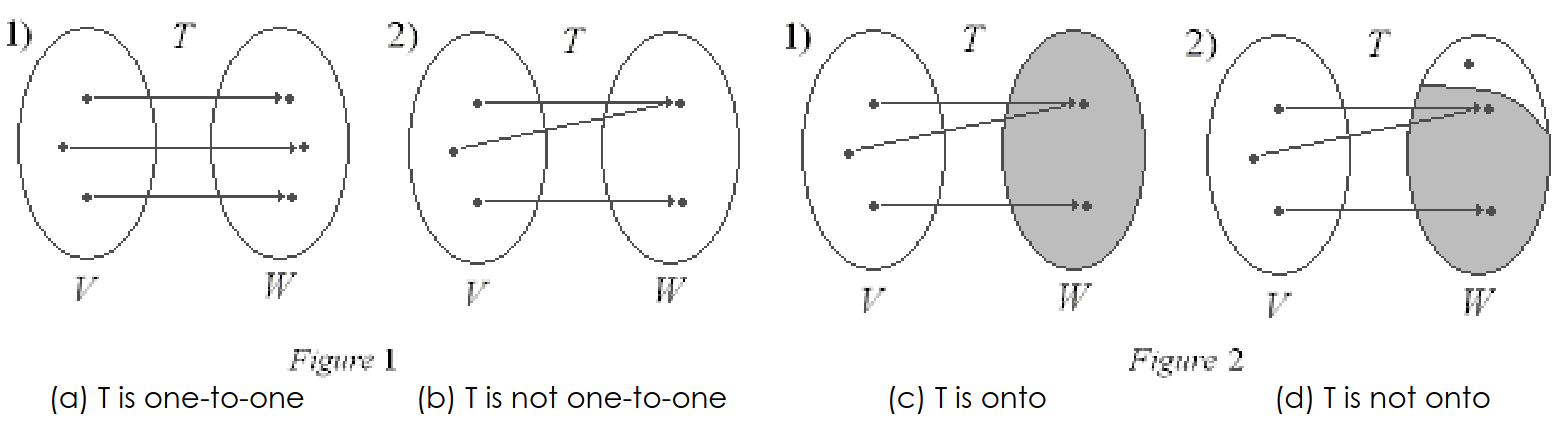
\includegraphics[width=1\linewidth]{linear-transformations.png}
\end{figure}

\begin{tikzpicture}
\node [rounded-box] (box){\begin{minipage}{0.975\textwidth}
    A linear transformation that is one-to-one and onto is called an \textbf{isomorphism} (iso = equal, morph = shape). If $V$ and $W$ are two vector spaces such that there is an isomorphism from $V$ to $W$, then $V$ is isomorphic to $W$:

    \vspace{-5pt}

    $$V \simeq W$$
\end{minipage}};
\node[rounded-box-title, left=10pt] at (box.north east) {Definition};
\end{tikzpicture}

\begin{tikzpicture}
\node [rounded-box] (box){\begin{minipage}{0.975\textwidth}
    Let $V, W$ be two finite-dimensional vector spaces (over the same field of scalars). Then $V$ is isomorphic to $W$ if and only if

    \vspace{-5pt}

    $$\text{dim}(V) = \text{dim}(W)$$
\end{minipage}};
\node[rounded-box-title, left=10pt] at (box.north east) {Theorem};
\end{tikzpicture}

\begin{tikzpicture}
\node [rounded-box] (box){\begin{minipage}{0.975\textwidth}
    Let $A$ be an $n \times n$ matrix. The following statements are equivalent:
    \begin{enumerate}
        \item $A$ is invertible.
        \item $A \mathbf{x} = \mathbf{b}$ has a unique solution for every $\mathbf{b} \in \mathbb{R}^n$.
        \item $A \mathbf{x} = \mathbf{0}$ has only the trivial solution.
        \item The reduced row echelon form of $A$ is $I_n$.
        \item $A$ is a product of elementary matrices.
        \item $\text{rank}(A) = n$.
        \item $\text{nullity}(A) = 0$.
        \item The column vectors of $A$ are linearly independent.
        \item The column vectors of $A$ span $\mathbb{R}^n$.
        \item The column vectors of $A$ form a basis for $\mathbb{R}^n$.
        \item The row vectors of $A$ are linearly independent.
        \item The row vectors of $A$ span $\mathbb{R}^n$.
        \item The row vectors of $A$ form a basis for $\mathbb{R}^n$.
        \item $\text{det}(A) \neq 0$.
        \item $0$ is not an eigenvalue of $A$.
        \item $T$ is invertible.
        \item $T$ is one-to-one.
        \item $T$ is onto.
        \item $\text{Ker}(T) = \{\mathbf{0}\}$.
        \item $\text{Range}(T) = W$.
    \end{enumerate}
\end{minipage}};
\node[rounded-box-title, left=10pt] at (box.north east) {The Fundamental Theorem of Invertible Matrices};
\end{tikzpicture}

\subsection{Inner Product Spaces}

\begin{tikzpicture}
\node [rounded-box] (box){\begin{minipage}{0.975\textwidth}
    The \textbf{inner product} takes pairs of vectors as inputs and produces scalars as outputs ($\mathbb{R}^n \times \mathbb{R}^n \rightarrow \mathbb{R}^n$):

    \vspace{-5pt}

    $$\mathbf{u}^T \mathbf{v} = \begin{bmatrix}
        u_1 & u_2 & u_3
    \end{bmatrix} \begin{bmatrix}
        v_1 \\ v_2 \\ v_3
    \end{bmatrix} = u_1 v_1 + u_2 v_2 + u_3 v_3$$
\end{minipage}};
\node[rounded-box-title, left=10pt] at (box.north east) {Definition};
\end{tikzpicture}

\begin{tikzpicture}
\node [rounded-box] (box){\begin{minipage}{0.975\textwidth}
    The \textbf{outer product} takes some vectors $\mathbf{u}, \mathbf{v}$ as inputs and produces matrices as outputs ($\mathbb{R}^n \times \mathbb{R}^n \rightarrow \mathbb{R}^{n \times n}$) such that every column is a multiple of the vector $\mathbf{u}$, and every row is a multiple of the vector $\mathbf{v}^T$:

    \vspace{-5pt}

    $$\mathbf{u} \mathbf{v}^T = \begin{bmatrix}
        u_1 \\ u_2 \\ u_3
    \end{bmatrix} \begin{bmatrix}
        v_1 & v_2 & v_3
    \end{bmatrix} = \begin{bmatrix}
        u_1 v_1 & u_1 v_2 & u_1 v_3 \\
        u_2 v_1 & u_2 v_2 & u_2 v_3 \\
        u_3 v_1 & u_3 v_2 & u_3 v_3
    \end{bmatrix}$$
\end{minipage}};
\node[rounded-box-title, left=10pt] at (box.north east) {Definition};
\end{tikzpicture}

\begin{tikzpicture}
\node [rounded-box] (box){\begin{minipage}{0.975\textwidth}
    An inner product on a vector space $V$ is an operation that assigns to every pair of vectors $\mathbf{u} , \mathbf{v} \in V$ a real number $\langle \mathbf{u}, \mathbf{v} \rangle$ such that the following properties hold for all vectors $\mathbf{u}, \mathbf{v}, \mathbf{w} \in V$ and all scalars $c$:

    \begin{itemize}
        \item $\langle \mathbf{u}, \mathbf{v} \rangle = \langle \mathbf{v}, \mathbf{u} \rangle$
        \item $\langle \mathbf{u}, \mathbf{v} + \mathbf{w} \rangle = \langle \mathbf{u}, \mathbf{v} \rangle + \langle \mathbf{u}, \mathbf{w} \rangle$
        \item $\langle c \mathbf{u}, \mathbf{v} \rangle = c \langle \mathbf{u}, \mathbf{v} \rangle$
        \item $\langle \mathbf{u}, \mathbf{u} \rangle \geq 0$
        \item $\langle \mathbf{u}, \mathbf{u} \rangle = 0$ if and only if $\mathbf{u} = \mathbf{0}$ \\
    \end{itemize}

    A vector space with such an inner product is called an \textbf{inner product space}.
\end{minipage}};
\node[rounded-box-title, left=10pt] at (box.north east) {Definition};
\end{tikzpicture}

\textbf{Example}: The dot product on $\mathbf{R}^n$ is an inner product.

\textbf{Example}: Continuous functions on an interval $[a, b]$ on the vector space $C[a, b]$ are inner products:

\begin{tikzpicture}
\node [rounded-box] (box){\begin{minipage}{0.975\textwidth}
    Let $f, g$ be continuous functions on an interval $[a, b]$. Then the inner product on the vector space $C[a, b]$ is defined as:

    $$
    \langle f, g \rangle = \int_a^b f(x) g(x) \, dx
    $$
\end{minipage}};
\node[rounded-box-title, left=10pt] at (box.north east) {Definition};
\end{tikzpicture}

\textbf{Example}: Let $f(x) = 1, g(x) = x^3$ on $C[0, 2]$. Their inner product is

$$
\langle f, g \rangle = \int_0^2 x^3 \, dx = \frac{1}{4} x^4 \Big{|}_0^2 = 4
$$

\begin{tikzpicture}
\node [rounded-box] (box){\begin{minipage}{0.975\textwidth}
    Let $\mathbf{u}, \mathbf{v}, \mathbf{w}$ be vectors in an inner product space $V$ and let $c$ be a scalar. Then

    \begin{itemize}
        \item $\langle \mathbf{u} + \mathbf{v}, \mathbf{w} \rangle = \langle \mathbf{u}, \mathbf{w} \rangle + \langle \mathbf{v}, \mathbf{w} \rangle$
        \item $\langle \mathbf{u}, c \mathbf{v} \rangle = c \langle \mathbf{u}, \mathbf{v} \rangle$
        \item $\langle \mathbf{u}, \mathbf{0} \rangle = \langle \mathbf{0}, \mathbf{v} \rangle = 0$
    \end{itemize}
\end{minipage}};
\node[rounded-box-title, left=10pt] at (box.north east) {Theorem};
\end{tikzpicture}

\begin{tikzpicture}
\node [rounded-box] (box){\begin{minipage}{0.975\textwidth}
    Let $\mathbf{u}, \mathbf{v}$ be vectors in an inner product space $V$. Then

    \begin{itemize}
        \item the \textbf{norm} or magnitude of $\mathbf{v}$ is: $|| \mathbf{v} || = \sqrt{\langle \mathbf{v}, \mathbf{v} \rangle}$
        \item their \textbf{distance} is: $d(\mathbf{u}, \mathbf{v}) = || \mathbf{u} - \mathbf{v} ||$
        \item $\langle \mathbf{u}, \mathbf{v} \rangle = 0 \iff \mathbf{u} \perp \mathbf{v}$
    \end{itemize}
\end{minipage}};
\node[rounded-box-title, left=10pt] at (box.north east) {Definition};
\end{tikzpicture}

Note: $|| \mathbf{v} ||$ is always defined, since $\langle \mathbf{v}, \mathbf{v} \rangle \geq 0$ by the definition of the inner product.

\textbf{Example}: Let $f(x) = 1, g(x) = x^3$ on $C[0, 2]$. Then their norms and distance are:

$$
|| f || = \sqrt{ \langle f, f \rangle } = \sqrt{ \int_0^2 f(x) f(x) \, dx } = \sqrt{ x \big{|}_0^2 } = \sqrt{2 - 0} = \sqrt{2}
\qquad
|| g || = \sqrt{ \langle g, g \rangle } = \sqrt{ \int_0^2 g(x) g(x) \, dx } = \sqrt{ x^7 / 7 \big{|}_0^2 } = \sqrt{2^7 / 7}
$$

$$
|| f - g || = \sqrt{ \langle f - g, f - g \rangle } = \sqrt{ \int_0^2 (f(x) - g(x))^2 \, dx }
$$

\textbf{Example}: Let $f(x) = 1, g(x) = \sin{x}$. In the vector space $C[0, \pi]$ with inner product $\langle f, g \rangle = \int_0^\pi f(x) g(x) \, dx$, are $f, g$ orthogonal?

\textbf{Example}: Let $f(x) = 1, g(x) = \sin{x}$. In the vector space $C[-\pi, \pi]$ with inner product $\langle f, g \rangle = \int_{-\pi}^\pi f(x) g(x) \, dx$, are $f, g$ orthogonal?

\begin{tikzpicture}
\node [rounded-box] (box){\begin{minipage}{0.975\textwidth}
    Let $\mathbf{u}, \mathbf{v}$ be vectors in an inner product space $V$. Then $\mathbf{u}, \mathbf{v}$ are orthogonal if and only if $|| \mathbf{u} + \mathbf{v} ||^2 = || \mathbf{u} ||^2 + || \mathbf{v} ||^2$.

    \begin{align}
        || \mathbf{u} + \mathbf{v} ||^2 & = \langle \mathbf{u} + \mathbf{v}, \mathbf{u} + \mathbf{v} \rangle \\
        & = \langle \mathbf{u} , \mathbf{u} \rangle + \langle \mathbf{u} , \mathbf{v} \rangle + \langle \mathbf{v} , \mathbf{u} \rangle + \langle \mathbf{v} , \mathbf{v} \rangle \\
        & = || \mathbf{u} ||^2 + 2 \langle \mathbf{u}, \mathbf{v} \rangle + || \mathbf{v} ||^2 \\
        & = || \mathbf{u} ||^2 + || \mathbf{v} ||^2 & \text{ if and only if } \langle \mathbf{u}, \mathbf{v} \rangle = 0
    \end{align}
\end{minipage}};
\node[rounded-box-title, left=10pt] at (box.north east) {The Pythagorean Theorem};
\end{tikzpicture}

\begin{paracol}{2}

\begin{tikzpicture}
\node [rounded-box] (box){\begin{minipage}{0.45\textwidth}
    Given a vector space $V$ with an inner product, a list $\{ v_1; v_2; \dots; v_n \}$ in $V$ is \textbf{orthogonal} if $\langle v_i, v_j \rangle = 0$ for all $i \neq j$. \\

    The list is orthonormal if it is orthogonal, and $|| v_i || = 1$ for all $i$.
\end{minipage}};
\node[rounded-box-title, left=10pt] at (box.north east) {Definition};
\end{tikzpicture}

\switchcolumn

\begin{tikzpicture}
\node [rounded-box] (box){\begin{minipage}{0.45\textwidth}
    Any orthogonal list of non-zero vectors is linearly independent.
\end{minipage}};
\node[rounded-box-title, left=10pt] at (box.north east) {Theorem};
\end{tikzpicture}

\end{paracol}
 \newpage

\nocite{*}
\printbibliography

\end{document}
